% =====================================================================================
% main.tex -- "Physics-informed neural networks and the Deep Ritz method for diffusion, wave
% and Laplace problems: a reproducible benchmark and its failure modes" (main text).
% The Supplementary Material is supplement.tex; the two documents refer to each other with
% xr-hyper (numbers with the prefix S are those of the supplement).
%
% Build (from this folder; PATH must contain the TeX Live binaries):
%   pdflatex supplement && pdflatex main && bibtex main && bibtex supplement
%   pdflatex supplement && pdflatex main && pdflatex supplement && pdflatex main
%   pdflatex supplement && pdflatex main
% (build_pdfs.sh runs this sequence, with three final passes, checks the logs and copies main.pdf to
% paper.pdf, the file to which the links of the supplement point.)
% Layout: macros.tex (notation), statements.tex (exact texts of the propositions),
%         sections/s*.tex (main text, one file per section), sections/S*.tex (supplement),
%         figures/, refs.bib.
% Every quantitative statement carries a comment  % src: <path>, relative to the root of the
% accompanying repository (reproduce.md there gives the command that regenerates each file):
%   data/, code/                    outputs and scripts of the article's own tables and figures
%   research_benchmark/, research_highdim/            the benchmark and the dimension study
%   research_highdim_bound/, research_highdim_remedies/  the stability constant with the error bound
%                                   (Section 6.7) and the two remedies (Section 6.8), each with the scripts
%                                   and outputs of its re-checks in check/
%   verify_research_benchmark/, verify_research_highdim/   the verification codes (Section 3.9)
%   notes/VERIFICATION.md, data/checks/   how the results were checked; records of the checks
% Floats: the option [section] of placeins keeps every figure and table inside its section, and
%         flafter keeps a float from being set above the place where it is defined.
% =====================================================================================
\documentclass[11pt,a4paper]{article}

\usepackage[T1]{fontenc}
\usepackage[utf8]{inputenc}
\usepackage{lmodern}
\usepackage[a4paper,margin=2.5cm]{geometry}
\usepackage{amsmath,amssymb,amsthm}
\usepackage{graphicx}
\usepackage{booktabs}
\usepackage{array}
\usepackage{caption}
\usepackage{flafter}
\usepackage[section]{placeins}
\usepackage{enumitem}
\usepackage{xcolor}
\usepackage{listings}
\usepackage[numbers,sort&compress]{natbib}
\usepackage{microtype}
\usepackage{xr-hyper}
\usepackage[colorlinks=true,linkcolor=blue!50!black,citecolor=blue!50!black,urlcolor=blue!50!black]{hyperref}
\externaldocument[][nocite]{supplement}[supplement.pdf]

\graphicspath{{figures/}}
\captionsetup{font=small,labelfont=bf}
\lstset{basicstyle=\ttfamily\small,columns=fullflexible,keepspaces=true,
        showstringspaces=false,frame=single,framerule=0.3pt,xleftmargin=1em,
        xrightmargin=1em,language=Python,breaklines=true}
\setlist{nosep}
\renewcommand{\bibfont}{\small}
\renewcommand{\topfraction}{0.9}
\renewcommand{\bottomfraction}{0.8}
\renewcommand{\textfraction}{0.08}
\renewcommand{\floatpagefraction}{0.85}
\setlength{\bibsep}{2pt plus 1pt}

% =====================================================================================
% macros.tex -- notation and theorem environments of the article.
% Loaded by main.tex after the packages.  Each quantity listed here has one symbol,
% used throughout the article.
%
% NOTATION TABLE
% -------------------------------------------------------------------------------------
%  symbol (macro)                meaning
% -------------------------------------------------------------------------------------
%  \Om, \dOm                     spatial domain Omega and its boundary
%  \QT                           space-time cylinder (0,T] x Omega (evolution problems)
%  d                             spatial dimension (Section 6: d = 2,...,20; cost up to 100;
%                                constants and bias up to d = 10^6)
%  \x                            point of Omega (bold x); x_i its coordinates
%  \lap, \grad, \dn              Laplacian, gradient, outward normal derivative
%  \uex                          exact solution u^*
%  \unet                         network approximation u_theta (theta = all weights)
%  \ubeta                        minimiser of the penalised Ritz energy with weight beta
%  \Lpinn                        PINN loss (empirical, eq. s3_methods:eq:pinn)
%  \Lpop                         population (continuum) PINN loss
%  \Eritz                        penalised Ritz energy E_beta (eq. s3_methods:eq:ritz)
%  \lam                          weight of the boundary term in the PINN loss
%                                (lambda = 1 in Sections 4-5; tuned in Section 6)
%  \bet                          boundary-penalty weight beta of the Deep Ritz energy
%  \Nr, \Nb, \Nic                numbers of interior (residual), boundary and
%                                initial-condition collocation points
%  \errL                         relative L2 error  ||u_theta-u^*||_2 / ||u^*||_2
%                                on the held-out evaluation set
%  \errI                         L-infinity error  max |u_theta-u^*| on the evaluation set
%  \errC                         centred relative L2 error ||u_theta-u^*|| / ||u^*-mean(u^*)||
%  \errH                         relative H1-seminorm error ||grad(u_theta-u^*)|| / ||grad u^*||
%  \errT(t)                      relative L2 error on the time slice t (heat problem)
%  \norm{.}, \abs{.}, \ip{.}{.}  norm, absolute value, L2 inner product
%  \R, \N                        real numbers, natural numbers
%  \dd                           upright differential d
%  \ee                           Euler's number (upright e)
%  \sci{a}{b}                    a x 10^b, e.g. \sci{1.6}{-3}
%  \PH, \PWone, \PWtwo,          problem names: Heat (1-D heat), Wave1 (two-mode 1-D wave),
%  \PLtwo, \PLthree,             Wave2 (2-D wave), Lap2 (2-D Laplace, mixed BC), Lap3 (3-D
%  \PLthreeS, \Pone, \Ptwo       Laplace, discontinuous data), Lap3s (3-D Laplace, compatible
%                                data), LapD (d-dim Laplace), PoiD (d-dim Poisson).
%  \Pridge, \Pcospair,          further problems on the unit cube of Section 6.8 (RidgeD,
%  \Paltridge, \Psinlin,         CosPairD, AltRidgeD; SinLinD, ExpCosD of the re-check), held
%  \Pexpcos                      out from the design of the two remedies tested there
%                                The digit is the space dimension.  The names are words so
%                                that they cannot be confused with the norm L^2, the space
%                                H^1 or the polynomial spaces P_0, P_1.
%  \strat{name}                  collocation strategy name, one of
%                                grid-c (cell-centred grid), grid-n (node-centred, closed grid),
%                                random (fixed i.i.d. uniform), resample (fresh i.i.d. uniform
%                                every Adam step), Sobol (scrambled Sobol', fixed),
%                                RAD (residual-based adaptive distribution)
%  \Adam, \LBFGS, \AdamLBFGS     optimiser arms: Adam; L-BFGS; Adam followed by L-BFGS
%  \nbd{.}                       norm of L2(dOmega) (surface measure)
%  \kappa_d                      norm of the harmonic extension L2(dOmega) -> L2(Omega) on the unit
%                                cube (Section 6.7); not the constant C_d = sqrt(1+1/(d pi^2)) of
%                                Proposition s3_methods:prop:robin(c)
%  U_d, L_d                      upper and lower bounds of kappa_d^2 (Theorem s6_highdim:thm:kappa)
%  \delta_1                      first biharmonic Steklov eigenvalue of the unit cube (= 1/kappa_d^2)
%  B_int, B_bd, \eta             interior and boundary terms of the computable error bound and its
%                                efficiency (bound over error), Corollary s6_highdim:cor:bound(c);
%                                eta is used for nothing else
%  \Lpop_int, \Lpop_bd           the two terms of the population PINN loss \Lpop_1 (mean squared residual,
%                                mean squared boundary misfit), Corollary s6_highdim:cor:bound(c)
%  m_d                           bound of kappa_d^2 through the torsion function \vartheta of the cube
%                                (-Lap theta = 1, theta = 0 on the boundary), Remark sA_proofs:rem:steklov
%  q, N                          q = d_n u^* on the boundary and N = ||q||_partial (Section S7.5)
%  M_\partial                    boundary Gram matrix of the affine functions (Section S7.6)
%  \mathcal A, \mathcal F, \mathcal S   affine functions, span of the lift features, additively separable
%                                functions (Section S7.6); sinc a = sin(a)/a
%  \rho                          seed-paired ratio err(plain)/err(arm) of Section 6.8
%  "plateau"                     (Section 6.8) a test error no smaller than the affine floor
%  "the re-check"                (Sections 6.7, 6.8, S5, S7) the two rounds of re-checks of the analyses of
%                                Sections 6.7 and 6.8, made with separately written code (Section 3.9)
%  \code{...}                    file names, identifiers (typewriter)
% -------------------------------------------------------------------------------------
% Terminology fixed for the whole article:
%   "iteration"   = one optimiser step (never "epoch");
%   "network"     = one trained network up to the point where the optimiser arms branch,
%                   i.e. one (problem, strategy, seed); "run" = one network in one arm;
%                   "pair" = the two runs of one network;
%   "held-out"    = evaluation points never used for training;
%   "seed"        = fixes initial weights and all random point sets of a run;
%   "relative L2 error" always means \errL on the held-out set unless a slice is named.
% =====================================================================================

% ---- sets, operators -------------------------------------------------------------
\newcommand{\R}{\mathbb{R}}
\newcommand{\N}{\mathbb{N}}
\newcommand{\dd}{\mathrm{d}}
\newcommand{\ee}{\mathrm{e}}
\newcommand{\Om}{\Omega}
\newcommand{\dOm}{\partial\Omega}
\newcommand{\QT}{Q_T}
\newcommand{\x}{\boldsymbol{x}}
\newcommand{\lap}{\Delta}
\newcommand{\grad}{\nabla}
\newcommand{\dn}{\partial_n}
\newcommand{\norm}[1]{\lVert #1\rVert}
\newcommand{\abs}[1]{\lvert #1\rvert}
\newcommand{\ip}[2]{\langle #1,\,#2\rangle}
\newcommand{\nbd}[1]{\norm{#1}_{\partial}}

% ---- solutions and functionals ---------------------------------------------------
\newcommand{\uex}{u^{*}}
\newcommand{\unet}{u_{\theta}}
\newcommand{\ubeta}{u_{\beta}}
\newcommand{\Lpinn}{\mathcal{L}}
\newcommand{\Lpop}{\mathcal{L}^{\mathrm{pop}}}
\newcommand{\Eritz}{\mathcal{E}_{\beta}}
\newcommand{\lam}{\lambda}
\newcommand{\bet}{\beta}

% ---- point budgets ---------------------------------------------------------------
\newcommand{\Nr}{N_{r}}
\newcommand{\Nb}{N_{b}}
\newcommand{\Nic}{N_{0}}

% ---- error measures --------------------------------------------------------------
\newcommand{\errL}{\varepsilon_{2}}
\newcommand{\errI}{\varepsilon_{\infty}}
\newcommand{\errC}{\varepsilon_{2}^{\mathrm{c}}}
\newcommand{\errH}{\varepsilon_{H^{1}}}
\newcommand{\errT}{\varepsilon_{2}^{\mathrm{slice}}}

% ---- numbers ---------------------------------------------------------------------
\newcommand{\sci}[2]{#1\times 10^{#2}}

% ---- names -----------------------------------------------------------------------
\newcommand{\PH}{\textsf{Heat}}
\newcommand{\PWone}{\textsf{Wave1}}
\newcommand{\PWtwo}{\textsf{Wave2}}
\newcommand{\PLtwo}{\textsf{Lap2}}
\newcommand{\PLthree}{\textsf{Lap3}}
\newcommand{\PLthreeS}{\textsf{Lap3s}}
\newcommand{\Pone}{\textsf{LapD}}
\newcommand{\Ptwo}{\textsf{PoiD}}
\newcommand{\Pridge}{\textsf{RidgeD}}
\newcommand{\Pcospair}{\textsf{CosPairD}}
\newcommand{\Paltridge}{\textsf{AltRidgeD}}
\newcommand{\Psinlin}{\textsf{SinLinD}}
\newcommand{\Pexpcos}{\textsf{ExpCosD}}
\newcommand{\strat}[1]{\textsf{#1}}
\newcommand{\Adam}{Adam}
\newcommand{\LBFGS}{L-BFGS}
\newcommand{\AdamLBFGS}{Adam$\,\to\,$L-BFGS}
\newcommand{\code}[1]{\texttt{\detokenize{#1}}}

% ---- theorem environments (amsthm) -----------------------------------------------
\theoremstyle{plain}
\newtheorem{theorem}{Theorem}
\newtheorem{proposition}[theorem]{Proposition}
\newtheorem{lemma}[theorem]{Lemma}
\newtheorem{corollary}[theorem]{Corollary}
\theoremstyle{definition}
\newtheorem{definition}[theorem]{Definition}
\newtheorem{observation}[theorem]{Numerical observation}
\newtheorem{conjecture}[theorem]{Conjecture}
\theoremstyle{remark}
\newtheorem{remark}[theorem]{Remark}

% =====================================================================================
% statements.tex -- the exact wording of every proposition of the article.
%
% A proposition is stated in one section and proved in Supplementary Section S7 (sections/S7_proofs.tex).
% So that statement and proof cannot drift apart, the text of each statement is kept here,
% once, as a macro.  The stating section writes
%     \begin{proposition}[<title>]\label{<label>}\StmtXxx\end{proposition}
% and Section S7 proves exactly that text, referring to the proposition by \ref.
%
%   macro            fixed label                      stated in      title
%   \StmtExact       s2_problems:prop:exact           s2_problems    Exact solutions
%   \StmtUnique      s2_problems:prop:unique          s2_problems    Uniqueness
%   \StmtFloors      s2_problems:prop:floors          s2_problems    Trivial-predictor floors
%   \StmtRobin       s3_methods:prop:robin            s3_methods     Penalised Ritz energy: Robin problem and penalty bias
%   \StmtNonunique   s7_pitfalls:prop:nonunique       s7_pitfalls    A Laplace problem with data on one face only
%   \StmtNotWave     s7_pitfalls:prop:notwave         s7_pitfalls    A decaying mode is not a wave solution
%   \StmtKappa       s6_highdim:thm:kappa             s6_highdim     The harmonic-extension constant of the unit cube
%   \StmtSteklov     s6_highdim:prop:steklov          s6_highdim     Biharmonic Steklov eigenvalue
%   \StmtCertificate s6_highdim:cor:bound             s6_highdim     (corollary) harmonic part, penalty bias, computable bound
%
% The statements use: problem names (macros.tex), Table s2_problems:tab:problems and
% equation s2_problems:eq:lap3d-exact (the series solution of Lap3), both defined in
% sections/s2_problems.tex, and equation s3_methods:eq:ritz (the penalised Ritz energy) of sections/s3_methods.tex.
% The three statements of Section 6.7 use the definition s6_highdim:eq:kappa of kappa_d and the PINN loss
% s3_methods:eq:pinn; the Lemma, Propositions and Theorem stated and proved inside Section S7 are written there.
% =====================================================================================

% ---------------------------------------------------------------- exact solutions ----
\newcommand{\StmtExact}{%
\begin{enumerate}
\item[(a)] For each of the problems \PH, \PWone, \PWtwo, \PLtwo, \PLthreeS, \Pone\ and \Ptwo\ of
Table~\ref{s2_problems:tab:problems}, the function $\uex$ listed there is infinitely
differentiable on the closed domain, satisfies the differential equation at every point,
and satisfies every initial and boundary condition pointwise.
\item[(b)] For \PLthree, let $k_n=\sqrt{1+n^2}$ and $b_n=4n/\bigl(\pi(n^2-1)\bigr)$ for even
$n\ge 2$. The series~\eqref{s2_problems:eq:lap3d-exact},
\[
\uex(x,y,z)=\sin y\sum_{n\ \mathrm{even}} b_n\,\sin(nz)\,
\frac{\sinh(k_n x)}{\sinh(k_n\pi)},
\]
converges, together with all its term-by-term derivatives, uniformly on
$[0,\pi-\delta]\times[0,\pi]^2$ for every $\delta\in(0,\pi)$. Its sum is harmonic in
$(0,\pi)^3$, belongs to $C^\infty\bigl([0,\pi)\times[0,\pi]^2\bigr)$, vanishes on the five
faces $\{x=0\}$, $\{y=0\}$, $\{y=\pi\}$, $\{z=0\}$, $\{z=\pi\}$, and attains the datum on
the sixth face in the mean-square sense,
\[
\lim_{x\to\pi^-}\int_0^\pi\!\!\int_0^\pi\bigl(\uex(x,y,z)-\sin y\cos z\bigr)^2\,\dd y\,\dd z=0 .
\]
The Dirichlet data of \PLthree\ are discontinuous along the two edges
$\{x=\pi,\ z=0\}$ and $\{x=\pi,\ z=\pi\}$, and $\uex$ has infinite Dirichlet energy,
$\int_{(0,\pi)^3}\abs{\grad\uex}^2\,\dd\x=\infty$.
\end{enumerate}}

% --------------------------------------------------------------------- uniqueness ----
\newcommand{\StmtUnique}{%
\begin{enumerate}
\item[(a)] Each of the problems \PH, \PWone, \PWtwo, \PLtwo, \PLthreeS, \Pone\ and \Ptwo\ has at
most one solution that is twice continuously differentiable on the closed domain (the
closed space--time cylinder for \PH, \PWone\ and \PWtwo). Hence the function $\uex$ of
Table~\ref{s2_problems:tab:problems} is the unique such solution.
\item[(b)] Problem \PLthree\ has at most one solution $u$ with the following three properties:
$u\in C^2\bigl([0,\pi)\times[0,\pi]^2\bigr)$ and $\lap u=0$ in $(0,\pi)^3$; $u=0$ on the five
faces $\{x=0\}$, $\{y=0\}$, $\{y=\pi\}$, $\{z=0\}$, $\{z=\pi\}$ (for $x<\pi$); and
$u(x,\cdot,\cdot)\to\sin y\cos z$ in $L^2\bigl((0,\pi)^2\bigr)$ as $x\to\pi^-$. The
series~\eqref{s2_problems:eq:lap3d-exact} is this solution.
\end{enumerate}}

% ------------------------------------------------------------------------ floors -----
\newcommand{\StmtFloors}{%
Let $\Om=(0,1)^d$ with $d\ge 2$, let $m=\lfloor d/2\rfloor$, and let $\norm{\cdot}$ be the
norm of $L^2(\Om)$. Write $\mathcal{P}_0$ for the constant functions and $\mathcal{P}_1$ for
the affine functions $\x\mapsto a_0+\sum_{i=1}^d a_i x_i$.
\begin{enumerate}
\item[(a)] For \Pone, $\uex=\sum_{k=1}^{m}x_{2k-1}x_{2k}$, one has
$\norm{\uex}^2=(9m^2+7m)/144$ and
\[
\min_{c\in\mathcal{P}_0}\frac{\norm{\uex-c}}{\norm{\uex}}=\sqrt{\frac{7}{7+9m}},\qquad
\min_{a\in\mathcal{P}_1}\frac{\norm{\uex-a}}{\norm{\uex}}=\sqrt{\frac{1}{7+9m}} .
\]
\item[(b)] For \Ptwo, $\uex=d^{-1/2}\sum_{i=1}^{d}\cos(\pi x_i)$, one has
$\norm{\uex}^2=\tfrac12$ for every $d$ and
\[
\min_{c\in\mathcal{P}_0}\frac{\norm{\uex-c}}{\norm{\uex}}=1,\qquad
\min_{a\in\mathcal{P}_1}\frac{\norm{\uex-a}}{\norm{\uex}}=\sqrt{1-\frac{96}{\pi^4}}\approx 0.1203,
\]
independently of $d$.
\end{enumerate}}

% ------------------------------------------------------------------------- Robin -----
\newcommand{\StmtRobin}{%
Let $\Om=(0,1)^d$, $f\in L^2(\Om)$, $g\in L^2(\dOm)$ and $\bet>0$, and let $\Eritz$ be the
penalised Ritz energy~\eqref{s3_methods:eq:ritz}, defined for $v\in H^1(\Om)$.
\begin{enumerate}
\item[(a)] $\Eritz$ has a unique minimiser $\ubeta\in H^1(\Om)$. It is characterised by
\[
\int_{\Om}\grad\ubeta\cdot\grad\varphi\,\dd\x+2\bet\int_{\dOm}(\ubeta-g)\,\varphi\,\dd s
=\int_{\Om}f\varphi\,\dd\x\qquad\text{for all }\varphi\in H^1(\Om),
\]
which is the weak form of the Robin problem
$-\lap u=f$ in $\Om$, $\ \dn u+2\bet\,(u-g)=0$ on $\dOm$.
\item[(b)] Assume that the Dirichlet problem $-\lap u=f$ in $\Om$, $u=g$ on $\dOm$ has a
solution $\uex\in C^2(\overline{\Om})$, and put $w=\ubeta-\uex$. Then
\[
\norm{\grad w}_{L^2(\Om)}^2+2\bet\,\norm{w}_{L^2(\dOm)}^2
=-\int_{\dOm}(\dn\uex)\,w\,\dd s ,
\]
and consequently
\[
\norm{w}_{L^2(\dOm)}\le\frac{\norm{\dn\uex}_{L^2(\dOm)}}{2\bet},\qquad
\norm{\grad w}_{L^2(\Om)}^2\le\frac{\norm{\dn\uex}_{L^2(\dOm)}^2}{8\bet}.
\]
\item[(c)] Under the assumption of (b),
\[
\norm{\ubeta-\uex}_{L^2(\Om)}\le\frac{C_d\,\norm{\dn\uex}_{L^2(\dOm)}}{\bet}
\qquad\text{for all }\bet>0,\qquad\text{with}\quad
C_d=\sqrt{1+\frac{1}{d\pi^2}}\le 1.05 .
\]
\item[(d)] Under the assumption of (b), $\ubeta=\uex$ for one (equivalently, for every)
$\bet>0$ if and only if $\dn\uex=0$ on $\dOm$.
\end{enumerate}
For \Pone\ one has $\norm{\dn\uex}_{L^2(\dOm)}^2=4m/3$ with $m=\lfloor d/2\rfloor$, so the
penalised minimiser is biased for every finite $\bet$; for \Ptwo\ one has $\dn\uex=0$, so
$\ubeta=\uex$ for every $\bet>0$.}

% ----------------------------------------------------------------- non-uniqueness ----
\newcommand{\StmtNonunique}{%
Let $D=(0,\pi)^3$. The boundary-value problem
\[
\lap u=0\ \text{ in }D,\qquad u(\pi,y,z)=\sin y\cos z\ \text{ for }(y,z)\in[0,\pi]^2,
\]
with no condition on the other five faces, has infinitely many solutions in
$C^\infty(\overline{D})$. Precisely:
\begin{enumerate}
\item[(a)] $u_0(x,y,z)=\cosh\bigl(\sqrt2\,(x-\pi)\bigr)\sin y\cos z$ is a solution;
\item[(b)] if $u$ is a solution and $h$ is a harmonic polynomial in the two variables $(y,z)$,
then $u+(x-\pi)\,h(y,z)$ is a solution; the solutions therefore form an affine space of
infinite dimension;
\item[(c)] for every $A\in\R$ the solution $u_0+A\,(x-\pi)$ takes the value $-A\pi$ at the
centre $(0,\pi/2,\pi/2)$ of the face $\{x=0\}$, so solutions exist whose values on the
unconstrained faces are arbitrarily large;
\item[(d)] the function $u_N(x,y,z)=\sin y\cos z\,\sinh(\sqrt2\,x)/\sinh(\sqrt2\,\pi)$, which
vanishes on $\{x=0\}$, $\{y=0\}$, $\{y=\pi\}$ and has zero normal derivative on $\{z=0\}$
and $\{z=\pi\}$, is another solution, different from $u_0$.
\end{enumerate}}

% ------------------------------------------------------------- not a wave solution ---
\newcommand{\StmtNotWave}{%
Let $\Om=(-1,1)^2$, $S(x,y)=\sin(\pi x)\sin(\pi y)$ and $\omega=\sqrt2\,\pi$.
\begin{enumerate}
\item[(a)] The function $v(t,x,y)=\ee^{-t}S(x,y)$ satisfies $v_{tt}-\lap v=(1+2\pi^2)\,\ee^{-t}S$,
which vanishes nowhere in $(0,\infty)\times\{S\neq 0\}$; $v$ is not a solution of the wave
equation $u_{tt}=\lap u$.
\item[(b)] The unique solution of \PWtwo\ is $\uex=\cos(\omega t)\,S$, and the relative distance
between $v$ and $\uex$ in $L^2\bigl((0,1)\times\Om\bigr)$ is
\[
\frac{\norm{v-\uex}}{\norm{\uex}}
=\Biggl(\frac{\int_0^1(\ee^{-t}-\cos\omega t)^2\,\dd t}{\int_0^1\cos^2\omega t\,\dd t}\Biggr)^{1/2}
\approx 1.380 .
\]
\end{enumerate}}

% ------------------------------------------------- remark: PINN loss is consistent ---
% (a remark, not a proposition; stated in s3_methods with label s3_methods:rem:consistent)
\newcommand{\StmtConsistent}{%
In contrast, consider the population PINN loss, the limit of the
loss~\eqref{s3_methods:eq:pinn} with one boundary block as the numbers of points grow.
Because every term of~\eqref{s3_methods:eq:pinn} is a mean, and $\abs{\Om}=1$ and
$\abs{\dOm}=2d$ for the unit cube, it is
\[
\Lpop_{\lam}(v)=\norm{\lap v+f}_{L^2(\Om)}^2+\frac{\lam}{\abs{\dOm}}\,\norm{v-g}_{L^2(\dOm)}^2 .
\]
For a function $v\in C^2(\overline{\Om})$ it vanishes if and only if $v$ solves the Dirichlet
problem, for every $\lam>0$: the exact solution is a global minimiser whatever the weight.
The weight $\lam$ changes the conditioning of the optimisation problem but not its
solution over $C^2(\overline{\Om})$, or over any class of functions that contains $\uex$,
whereas $\bet$ changes the solution of the penalised Ritz problem itself. Over a class that
does not contain $\uex$, such as a network of fixed size, the minimiser of $\Lpop_{\lam}$
does in general depend on $\lam$, because the residual and the boundary misfit are traded
against each other.
The two weights are also normalised differently: $\lam$ multiplies a mean over the
boundary and $\bet$ an integral over it, so that one boundary sample carries the weight
$\lam/\Nb$ in~\eqref{s3_methods:eq:pinn} and $2d\,\bet/\Nb$
in~\eqref{s3_methods:eq:ritz-mc}. At fixed $(\lam,\bet)$ the boundary weight of Deep Ritz
relative to that of the PINN therefore grows like $2d$.}

% ------------------------------------------------- harmonic-extension constant (Section 6.7) ---
\newcommand{\StmtKappa}{%
Let $\kappa_d$ be defined by~\eqref{s6_highdim:eq:kappa}. For $d\ge1$,
\[
\max\Bigl\{L_d,\frac1{2d}\Bigr\}\le\kappa_d^2\le U_d,
\]
where
\[
U_d=\frac{\tanh\bigl(\pi\sqrt{d-1}/2\bigr)}{\pi\sqrt{d-1}}\ \ (d\ge2),\quad U_1=\tfrac12,\qquad
L_d=\frac4{\pi^2}\sum_{j\ \mathrm{odd}}\frac{j^2}{(j^2+d-1)^2}.
\]
Moreover $\kappa_1^2=\frac12$, and $U_d<\frac12$ for $d\ge2$. As $d\to\infty$, $\sqrt d\,U_d\to1/\pi$ and
$\sqrt d\,L_d\to1/(2\pi)$, so $\kappa_d^2$ is of exact order $d^{-1/2}$.}

\newcommand{\StmtSteklov}{%
Let $\Om=(0,1)^d$ and
$\delta_1=\inf\{\norm{\lap u}^2/\nbd{\dn u}^2:\ u\in H^2(\Om)\cap H^1_0(\Om),\ \dn u\ne0\}$, the
variational form of the first eigenvalue of the biharmonic Steklov problem $\lap^2u=0$ in $\Om$, $u=0$ and
$\lap u=\delta_1\dn u$ on $\dOm$~\citep[(2.2)]{bucur2011first}. Then $\kappa_d^2=1/\delta_1$; hence
$1/U_d\le\delta_1\le\min\{1/L_d,2d\}$.}

\newcommand{\StmtCertificate}{%
Let $\Om=(0,1)^d$ and let $\uex\in C^2(\overline\Om)$ solve $-\lap\uex=f$ in $\Om$, $\uex=g$ on $\dOm$.
\begin{enumerate}
\item[(a)] Every $w\in H^1(\Om)$ with $\int_\Om\grad w\cdot\grad\varphi\,\dd\x=0$ for all
$\varphi\in H^1_0(\Om)$ satisfies $\norm{w}\le\kappa_d\nbd{w}\le\sqrt{U_d}\,\nbd{w}$.
\item[(b)] The minimiser $\ubeta$ of the penalised Ritz energy~\eqref{s3_methods:eq:ritz} satisfies
$\norm{\ubeta-\uex}\le\sqrt{U_d}\,\nbd{\dn\uex}/(2\bet)$ for every $\bet>0$.
\item[(c)] For every $v\in C^2(\overline\Om)$, in particular every network with $\tanh$ activations,
\begin{align*}
\norm{v-\uex}&\le\underbrace{\frac{\norm{\lap v+f}}{d\pi^2}}_{B_{\mathrm{int}}}
+\underbrace{\sqrt{U_d}\,\nbd{v-g}}_{B_{\mathrm{bd}}}
=\frac{\sqrt{\Lpop_{\mathrm{int}}(v)}}{d\pi^2}+\sqrt{2dU_d}\,\sqrt{\Lpop_{\mathrm{bd}}(v)},
\end{align*}
where $\Lpop_{\mathrm{int}}(v)=\norm{\lap v+f}^2$ and $\Lpop_{\mathrm{bd}}(v)=\nbd{v-g}^2/\abs{\dOm}$ are the
mean squared interior residual and the mean squared boundary misfit over the uniform measures, the two
terms of the population PINN loss $\Lpop_1$ of Remark~\ref{s3_methods:rem:consistent}.
\end{enumerate}}


\hypersetup{
  pdftitle={Physics-informed neural networks and the Deep Ritz method for diffusion, wave and Laplace problems: a reproducible benchmark and its failure modes},
  pdfauthor={Xiaoxiao Zhouyi},
  pdfkeywords={physics-informed neural networks, Deep Ritz method, collocation sampling, L-BFGS, finite-difference baselines, high-dimensional Poisson equation, a posteriori error bound, biharmonic Steklov eigenvalue, reproducibility}
}

\title{Physics-informed neural networks and the Deep Ritz method for diffusion, wave and
Laplace problems: a reproducible benchmark and its failure modes}

\author{Xiaoxiao Zhouyi\\[0.4em]
\small School of Engineering Mathematics and Technology, University of Bristol, UK.\\
\small \href{mailto:zhouyixiaoxiao@gmail.com}{\texttt{zhouyixiaoxiao@gmail.com}}}

\date{}

\begin{document}
\maketitle

% ------------------------------------------------------------------------ abstract ---
% Every number of the abstract is stated again, with its source, in the body; the
% src comments below repeat the sources.  code/check_headline_numbers.py checks them.
\begin{abstract}
\noindent
% src: research_benchmark/results/tables.md (T2); research_benchmark/results/stats.json; research_benchmark/results/tables.md (T3, T6); data/s4_lowdim_gridcontrol.json
We benchmark physics-informed neural networks (PINNs) and the Deep Ritz method on eight linear
problems (dimension $d\le20$) with exact solutions proved unique in a stated class, using seeded paired runs and low-dimensional classical baselines. An \LBFGS\
phase after \Adam\ lowers the error in all 175 pairs; the largest collocation
penalty after it (cell-centred grid, heat problem) comes from missing points near the
initial line.
% src: research_benchmark/results/benchmark_runs.csv (wave1d: 50 runs, 0.414 to 0.512); data/s5_hard_wave1d_long.json; data/s5_hard_cost.json (summary: ratio_smallest_of_all_measurements 475.6; fd_error_over_pinn_error_range 0.11 to 0.47)
A small unit-weight PINN fails on a two-mode wave problem; finite differences are over
400 times faster at equal or better accuracy.
% src: research_highdim/results/summary.csv; research_highdim/results/extensions.json (equaltime, d = 10)
The PINN is more accurate per iteration up to $d=10$, Deep Ritz at equal CPU time at $d=10$.
% src: sections/s6_highdim.tex (Theorem s6_highdim:thm:kappa, Corollary s6_highdim:cor:bound); data/s6_highdim_bound_numbers.json (n_networks_bound_valid, eta_d10_d20_all_networks, eta_by_d_all_networks: d = 2 max 24.82); research_highdim_bound/results/decisions.json (H2: 21 of 57)
On the unit cube we prove that the harmonic-extension norm from the boundary has exact order
$d^{-1/4}$; with it, as already with Payne's constant, the two population PINN loss terms bound
the $L^2$ error of any $C^2$ network. The bound held on all 133 networks, exceeding the error
1.9 to 3.4 times at $d\ge10$, up to 25 at $d=2$, missing a pre-registered
target ($\le3$ for $d\ge5$) on 21 of 57 networks.
% src: research_highdim_remedies/results/summary.json (P2/d20 plain, presolve, lift3c, rep3); research_highdim_remedies/results/summary_exploratory.json (P2/d20 lift1); research_highdim_remedies/results/decision.json (general_lift3c); research_highdim_remedies/results/decision_p5.json; research_highdim_remedies/results/checks.json (C5_floors poisson/d20: test_affine, exact_lift3 3.9e-3); research_highdim_remedies/results/summary_p5.json (P5/d20 lift3c, presolve)
At $d=20$ Legendre input features (containing the Poisson solution to 0.4 per cent), centred
inputs (exploratory) and, for Deep Ritz, a featureless reparametrisation each remove a plateau
left by a fixed affine part. The features passed a pre-registered generality test on four
problems but, like the affine part, hurt on a fifth problem, added afterwards (not blind).
Minimal examples show two pitfalls: a residual zeroed by misused automatic differentiation, and
too few boundary conditions.
\end{abstract}

\noindent\textbf{Keywords:} physics-informed neural networks; Deep Ritz method; collocation
sampling; L-BFGS; finite-difference baselines; high-dimensional Poisson equation; a posteriori
error bound; biharmonic Steklov eigenvalue; reproducibility.

% ------------------------------------------------------------------------ sections ---
% =====================================================================================
% sections/s1_intro.tex -- Introduction (body only).
% The contributions are stated without numbers; the numbers are in Sections 4 to 7 and,
% once, in Section 8.1.  No figures, tables or new computation.
% =====================================================================================
\section{Introduction}\label{s1_intro:sec}

A physics-informed neural network (PINN) represents the solution of a partial
differential equation by a neural network whose weights minimise the squared residual of
the equation at collocation points, plus the misfit to the initial and boundary
data~\citep{raissi2019}; neural trial functions for differential equations go back at least
to \citet{lagaris1998}. The Deep Ritz method~\citep{eyu2018} minimises instead a
Monte-Carlo estimate of the variational energy of an elliptic problem, with the boundary
condition imposed by a penalty. Both methods need no mesh, only automatic differentiation;
they are short to implement~\citep{lu2021} and extend formally to inverse
problems~\citep{raissi2019} and to high dimension~\citep{sirignano2018}, where other
neural solvers exist as well~\citep{han2018}; see the
reviews~\citep{karniadakis2021,cuomo2022}.

Their difficulties are equally well documented. The terms of a PINN loss can be badly
unbalanced~\citep{wangteng2021}; a neural-tangent-kernel analysis shows that they are then
learnt at different rates and exhibits a two-mode wave problem on which the unweighted
method fails~\citep{wangyu2022}, which we reuse as problem \PWone. PINNs that succeed on simple
linear equations fail as the coefficients grow, for reasons of optimisation rather than
expressivity~\citep{krishnapriyan2021}, and time-dependent problems may need a loss that
respects causality~\citep{wangsankaran2024}. Quasi-Newton optimisation has been part of
the method since \citet{raissi2019}; \citet{rathore2024} measure the benefit of running
\Adam\ and then \LBFGS\ and relate it to the ill-conditioning of the loss. The placement of collocation
points has been compared systematically by \citet{wu2023}, with residual-based refinement
and importance sampling as adaptive variants~\citep{lu2021,nabian2021}; \citet{daw2023}
attribute failures of PINNs to a failed propagation of the solution from the initial and
boundary points into the interior. Against classical
solvers, PINNs did not beat the finite element method in solution time and accuracy in the
study of \citet{grossmann2024}; \citet{mcgreivy2024} show that weak baselines and selective
reporting have made machine-learning solvers for fluid-related equations look better than
they are; and much larger benchmarks than ours exist~\citep{hao2023pinnacle}. On the theoretical side, PINN
minimisers converge for linear elliptic and parabolic problems as the number of collocation
points grows~\citep{shin2020}, and a boundary penalty is known to change the problem being
solved~\citep{babuska1973,muller2022}.

This article asks what the two methods deliver on the diffusion, wave and Laplace equations
when every error is measured against an exact solution, every run is seeded, comparisons are
paired and a classical solver is run alongside, and it contributes the following.
\begin{enumerate}[label=(C\arabic*),leftmargin=*]
\item Eight test problems, each stated so that it has a unique solution in a stated class:
the unique classical solution or, for the three-dimensional problem with discontinuous
data, the unique solution that attains the datum in mean square. The exact solutions are
given with proofs (Section~\ref{s2_problems:sec}; Supplementary
Sections~\ref{S1:sec} and~\ref{sA_proofs:sec}).
% src: research_benchmark/results/benchmark_runs.csv (350 rows = 175 networks x 2 arms)
\item A seeded benchmark of 175 networks on five low-dimensional problems, with five
collocation strategies and two optimiser arms of equal length, reporting held-out relative
errors; for the heat equation the error is also resolved in time, which shows how a small
space--time error hides a large error at late times (Sections~\ref{s3_methods:sec}
and~\ref{s4_lowdim:sec}).
\item The effect of replacing the second half of the \Adam\ iterations by \LBFGS, measured
pair by pair and also against the best logged \Adam\ iterate
(Section~\ref{s4_lowdim:sec:optimiser}).
\item A paired comparison of the collocation strategies, with a control experiment that
traces the one large penalty after the \LBFGS\ phase, that of a cell-centred grid on the
heat problem, to the absence of residual points next to the initial line
(Section~\ref{s4_lowdim:sec:strategy}).
\item Longer runs and a compatible-data control on the two- and three-dimensional problems,
which show what limits them; runs of up to 41\,000 iterations showing that the two-mode wave
problem is not solved by the unit-weight PINN at the network size used, with the trained
networks projected onto the two modes; and a comparison of all five problems with
second-order finite differences in accuracy and time (Section~\ref{s5_hard:sec}).
\item A comparison of the PINN and the Deep Ritz method on the unit cube in dimension $d=2$
to $20$, in accuracy per iteration, in cost per iteration, at equal compute and at two
budgets, with the penalty bias of Deep Ritz computed exactly
(Sections~\ref{s6_highdim:sec:equal-its}--\ref{s6_highdim:sec:weights}).
\item On the unit cube in any dimension $d$, two-sided bounds of exact order $d^{-1/2}$ for
the squared norm of the harmonic extension from $L^2(\dOm)$, with surface measure, to
$L^2(\Om)$, which is the inverse of the first biharmonic Steklov eigenvalue. With them the
$L^2$ error of any network is bounded by the two terms of the PINN loss with a constant
explicit in $d$, and the penalty bias of Deep Ritz by a sharper constant. The bound is
evaluated under a pre-registered protocol on the trained networks of the dimension study
and, without pre-registration, on networks retrained with separately written code
(Section~\ref{s6_highdim:sec:bound}).
\item A pre-registered test, for both methods, at equal iterations and at equal CPU time,
with two pre-registered controls for Deep Ritz (lift3u, rep3) and an exploratory centred-input
arm for both methods, of two cheap remedies for the plateau at
$d=20$, where neither method improves on the best affine approximation of the solution: a
fixed affine part computed by one linear solve, and coordinate-wise Legendre input features
(Section~\ref{s6_highdim:sec:remedies}).
\item Two implementation pitfalls demonstrated on minimal, released examples: a PDE
residual made identically zero by differentiating with respect to a slice of the input and
replacing the missing derivative by zeros, and a
boundary-value problem with too few conditions, on which training reaches a small loss with
a different function for every seed (Section~\ref{s7_pitfalls:sec}).
\end{enumerate}

The study combines a dimension-explicit stability result with controlled measurements of
established neural PDE solvers. The two-sided bound in (C7) is the theoretical contribution;
the experiments connect optimiser choice, sampling, error reporting and computational cost
within one reproducible protocol.
% src: refs.bib (rathore2024, annote: Sec. 2.2 and Table 1 of arXiv:2402.01868v2, checked 2026-10-01)
The gain from an \LBFGS\ phase after \Adam\ was measured by \citet{rathore2024}; what is
added here is the same measurement, paired by seed, on the heat and Laplace problems at a
small budget and against an untuned \Adam\ (Section~\ref{s4_lowdim:sec:optimiser}).
% src: research_benchmark/results/tables.md (T3: sobol/random after Adam -> L-BFGS 0.97, 0.54, 1.00, 0.99, 0.78; 10 of 10 seeds on no problem)
That the point set matters mainly when points are scarce is in the direction reported by
\citet{wu2023}; at our much smaller budgets we do not reproduce their ranking of grid and
resampled points on every problem. That a PINN needs residual points next to the initial
data (C4) is consistent with the propagation hypothesis of \citet{daw2023} and with causal
training~\citep{wangsankaran2024}; the control experiment isolates it for one problem. The
late-time behaviour of the heat problem (C2) is an elementary consequence of a loss made of
absolute residuals; the time-slice analysis quantifies its size on this test problem. The cost gap to classical solvers agrees with \citet{grossmann2024}, and
the penalty bias is classical~\citep{babuska1973,muller2022}. The residual loss and the Ritz
loss have been compared on elliptic problems by \citet{chen2020comparison}, who found, as we
do, that neither dominates the other. The constant of (C7) is classical: it is
$\delta_1^{-1/2}$ for the first biharmonic Steklov eigenvalue $\delta_1$, Payne's bound for
convex domains~\citep{payne1968bounds}, as stated in~\citet[Lemma~5.3]{bucur2011first}, already
gives a constant independent of $d$, and the torsion function of the cube gives one that
decreases slowly with $d$; to our knowledge, what is new is the explicit two-sided bound of
the squared constant $1/\delta_1$ of exact order $d^{-1/2}$ on the cube (equivalently, the
constant itself is of exact order $d^{-1/4}$). The error bound that
follows is an application of known theory with a better constant: a bound of the same form,
on smooth domains and with a constant that is not explicit, is in
\citet[App.~B]{shin2023error}. The remedies of (C8) use established
constructions~\citep{lagaris1998,ainsworth2021galerkin,chang2022horderdnn,zhang2025khorderdnn};
the paired comparisons measure their benefits and failure cases under a common budget.
The empirical contribution is the combination of
exact solutions, seeds, paired comparisons and a classical baseline of the kind whose
absence \citet{mcgreivy2024} criticise; a verification of the benchmark and of the dimension
study by re-aggregation of the raw runs and by separately written code for part of them
(Section~\ref{s3_methods:sec:verif} states what it covers and what it does not); and the
release of all code and data.

The experiments cover linear, constant-coefficient problems on boxes; the
networks are small and use the tanh activation; the loss weights are equal to one in
Sections~\ref{s4_lowdim:sec} and~\ref{s5_hard:sec}, and a single boundary weight per problem
and method is chosen once in Section~\ref{s6_highdim:sec}. Of the published remedies only two
cheap ones were tried, at $d=20$; adaptive loss weights, causal training, Fourier features and
boundary conditions built into the trial function were not
(Section~\ref{s8_discussion:sec:nottried}). Each of these might change a conclusion, in
particular the outcome on \PWone:
% src: refs.bib (rathore2024, annote: App. A.3, beta = 5; Sec. 2.2: widths up to 400, 10000 residual points, tuned Adam rate, switch after 1000, 11000 or 31000 Adam iterations; Table 1: lowest loss over widths after tuning)
on a variant with a faster second mode, \citet{rathore2024} report a few per cent with a
larger network and budget and tuned settings, without any of these remedies
(Section~\ref{s5_hard:sec:w1}).

Section~\ref{s2_problems:sec} states the problems and Section~\ref{s3_methods:sec} the
methods. Sections~\ref{s4_lowdim:sec}, \ref{s5_hard:sec} and~\ref{s6_highdim:sec} report
the low-dimensional benchmark, the harder problems with the finite-difference baselines,
and the dimension study, including the stability constant with the computable error bound
(Section~\ref{s6_highdim:sec:bound}) and the two remedies
(Section~\ref{s6_highdim:sec:remedies}). Section~\ref{s7_pitfalls:sec} demonstrates the two
implementation pitfalls, and Section~\ref{s8_discussion:sec} discusses the evidence and its
limitations. The Supplementary Material contains the proofs
(Section~\ref{sA_proofs:sec}), further results, figures and tables for each section, and
implementation details with full tables (Section~\ref{sC_details:sec}); its sections,
equations, figures and tables carry the prefix S.

% =====================================================================================
% sections/s2_problems.tex -- Test problems and exact solutions.
% All `% src:` paths are relative to the root of the repository.
% The statements of Propositions s2_problems:prop:exact and :prop:unique, the further checks of
% the exact solutions and the coincidences of evaluation and training points are in the
% Supplementary Material (sections/S1_problems.tex).
% =====================================================================================
\section{Test problems and exact solutions}\label{s2_problems:sec}

We use eight linear, constant-coefficient problems on boxes. Each has an exact solution in
closed form or, in one case, as a series, so every error reported below is measured
against the true solution and not against another numerical method. Five problems are
low-dimensional (\PH, \PWone, \PWtwo, \PLtwo, \PLthree), one is a control variant of
\PLthree\ with compatible data (\PLthreeS), and two are posed on the unit cube in any
dimension $d\ge 2$ (\Pone, \Ptwo). Table~\ref{s2_problems:tab:problems} lists them with their
origin and the held-out evaluation set; the networks are in
Table~\ref{s3_methods:tab:setup}. In the evolution problems $t$ is the
first coordinate and $\lap$ acts on the space variables only. The evaluation sets are dense
grids, or random points drawn from a generator of their own, and are separate from the
training points except for a few grid nodes on the boundary and, for \PLthree, the points of
one collocation strategy (Supplementary Section~\ref{S1:sec}).

% -------------------------------------------------------------------------------------
% Table of problems.
% src (equations, data, exact solutions, evaluation sets of Heat, Wave1, Wave2, Lap2, Lap3):
%      research_benchmark/pinnbench/problems.py
% src (Lap3s): code/s5_hard_laplace3d_smooth.py (same network and evaluation grid as Lap3)
% src (LapD, PoiD, 50 000 test points): research_highdim/scripts/hd_core.py
%      (exact, source, fixed_sets)
% src (origins): refs.bib annotations of strauss2008 (Sec. 6.2: exercise for Lap2; setting for the cube),
%      wangyu2022 and eyu2018 (eyu2018: Sec. 3.2 for LapD, Sec. 3.3 for the solution of PoiD;
%      arXiv:1710.00211 read on 2026-10-01)
% -------------------------------------------------------------------------------------
\begin{table}[tp]
\centering
\caption{The eight test problems. Evaluation set: the held-out points on
which all errors are computed; grids are uniform and include the boundary unless they are
cell-centred. In \Pone\ and \Ptwo\ the Dirichlet datum is the restriction of $\uex$ to $\dOm$.
The networks are listed in Table~\ref{s3_methods:tab:setup}.}
\label{s2_problems:tab:problems}
\footnotesize
\setlength{\tabcolsep}{2.6pt}
\renewcommand{\arraystretch}{1.3}
\begin{tabular}{@{}l
  >{\raggedright\arraybackslash}p{2.0cm}
  >{\raggedright\arraybackslash}p{3.35cm}
  >{\raggedright\arraybackslash}p{3.4cm}
  >{\raggedright\arraybackslash}p{3.3cm}
  >{\raggedright\arraybackslash}p{1.9cm}@{}}
\toprule
 & Equation, domain & Data & Exact solution $\uex$ & Origin & Evaluation set\\
\midrule
\PH & $u_t=u_{xx}$; $x\in(0,1)$, $t\in(0,1]$
    & $u(0,x)=\sin\pi x$; $u(t,0)=u(t,1)=0$
    & $\ee^{-\pi^2t}\sin\pi x$
    & standard single mode
    & $201\times201$ grid in $(t,x)$\\
\PWone & $u_{tt}=4u_{xx}$; $x\in(0,1)$, $t\in(0,1]$
    & $u(0,x)=\sin\pi x$ ${}+\tfrac12\sin4\pi x$; $u_t(0,x)=0$; $u(t,0)=u(t,1)=0$
    & $\sin\pi x\cos2\pi t$ ${}+\tfrac12\sin4\pi x\cos8\pi t$
    & \citet{wangyu2022}, Sec.~7.3
    & $201\times201$ grid in $(t,x)$\\
\PWtwo & $u_{tt}=\lap u$; $\Om=(-1,1)^2$, $t\in(0,1]$
    & $u(0,\cdot)=\sin\pi x\sin\pi y$; $u_t(0,\cdot)=0$; $u=0$ on $\dOm$
    & $\sin\pi x\,\sin\pi y\,\cos(\sqrt2\,\pi t)$
    & standard standing mode
    & $21\times81\times81$ grid in $(t,x,y)$\\
\PLtwo & $\lap u=0$; $\Om=(0,\pi)^2$
    & $u(0,y)=0$; $u(\pi,y)=\tfrac12(1+\cos2y)$; $u_y(x,0)=u_y(x,\pi)=0$
    & $\displaystyle\frac{x}{2\pi}+\frac{\cos2y\,\sinh2x}{2\sinh2\pi}$
    & \citet{strauss2008}, Sec.~6.2, Ex.~3
    & $201\times201$ grid\\
\PLthree & $\lap u=0$; $\Om=(0,\pi)^3$
    & $u(\pi,y,z)=\sin y\cos z$; $u=0$ on the other five faces
    & series~\eqref{s2_problems:eq:lap3d-exact}
    & the setting of \citet{strauss2008}, Sec.~6.2
    & $40^3$ cell centres\\
\PLthreeS & $\lap u=0$; $\Om=(0,\pi)^3$
    & $u(\pi,y,z)=\sin y\sin z$; $u=0$ on the other five faces
    & $\displaystyle\sin y\,\sin z\,\frac{\sinh(\sqrt2\,x)}{\sinh(\sqrt2\,\pi)}$
    & control variant of \PLthree
    & $40^3$ cell centres\\
\Pone & $\lap u=0$; $\Om=(0,1)^d$
    & $u=\uex$ on $\dOm$
    & $\sum_{k=1}^{\lfloor d/2\rfloor}x_{2k-1}x_{2k}$
    & \citet{eyu2018}, Sec.~3.2 ($d=10$)
    & $50\,000$ uniform random points\\
\Ptwo & $-\lap u=\pi^2\uex$; $\Om=(0,1)^d$
    & $u=\uex$ on $\dOm$
    & $d^{-1/2}\sum_{i=1}^{d}\cos\pi x_i$
    & solution of \citet{eyu2018}, Sec.~3.3 (a Neumann problem, $d=5,10$), rescaled; posed here as a Dirichlet problem
    & $50\,000$ uniform random points\\
\bottomrule
\end{tabular}
\end{table}

\paragraph{Heat equation.}
% src: data/closed_forms.json (heat1d.exp_minus_pi2 = 5.1723e-05, heat1d.exp_plus_pi2 = 19333.69)
The solution of \PH\ decays to $\ee^{-\pi^2}=\sci{5.17}{-5}$ of its initial size at $t=1$. Since
$\norm{\uex(t,\cdot)}_{L^2(0,1)}=\ee^{-\pi^2 t}/\sqrt2$, a given $L^2$ error on the time
slice $t$ is a relative error $\sqrt2\,\ee^{\pi^2 t}$ times as large on that slice, a factor
$\ee^{\pi^2}\approx\sci{1.93}{4}$ larger at $t=1$ than at $t=0$. A small space--time
relative error $\errL$ therefore says little about late times, and we also report the
relative error $\errT(t)$ on single time slices (both are defined
in~\eqref{s3_methods:eq:errors}; results in Section~\ref{s4_lowdim:sec:timeslice}).

\paragraph{Wave equations.}
Problem \PWone\ is the benchmark of \citet[Sec.~7.3]{wangyu2022}:
\begin{equation}\label{s2_problems:eq:wave1d}
u_{tt}=4u_{xx},\quad u(t,0)=u(t,1)=0,\quad u(0,x)=\sin\pi x+\tfrac12\sin4\pi x,\quad
u_t(0,x)=0 .
\end{equation}
It superposes two standing modes with amplitudes $1$ and $\tfrac12$ and frequencies in the
ratio $1:4$: on $0\le t\le 1$ the first completes one period and the second four.
Problem \PWtwo\ is the two-dimensional wave equation
\begin{equation}\label{s2_problems:eq:wave2d}
u_{tt}=\lap u\ \text{in }(-1,1)^2,\quad u=0\ \text{on }\dOm,\quad
u(0,x,y)=\sin\pi x\,\sin\pi y,\quad u_t(0,x,y)=0 .
\end{equation}
% src: data/closed_forms.json (wave2d.omega = 4.4429, wave2d.exact_factor_at_t_1_2_3[0] = -0.26626)
Its solution is a single standing mode of period $\sqrt2$, so $0\le t\le 1$ covers
$1/\sqrt2\approx 0.71$ of one period; the solution changes sign at $t=1/(2\sqrt2)\approx 0.35$
and its amplitude factor at $t=1$ is $\cos(\sqrt2\,\pi)=-0.266$. A function that only decays
in time is therefore far from the solution.

\paragraph{Laplace problems.}
Problem \PLtwo\ (Exercise~3 of Section~6.2 of \citet{strauss2008}) mixes Dirichlet data on two
sides with homogeneous Neumann data on the other two. The data are compatible at the four
corners, because both Dirichlet data have zero $y$-derivative at $y=0$ and $y=\pi$, and the
solution is smooth up to the boundary. Problem \PLthree,
\begin{equation}\label{s2_problems:eq:lap3d}
\lap u=0\quad\text{in }\Om=(0,\pi)^3;\qquad u(\pi,y,z)=\sin y\,\cos z,\qquad
u=0\ \text{on the other five faces,}
\end{equation}
is solved by separation of variables:
\begin{equation}\label{s2_problems:eq:lap3d-exact}
\uex(x,y,z)=\sin y\sum_{n\ \mathrm{even}} b_n\,\sin(nz)\,\frac{\sinh(k_n x)}{\sinh(k_n\pi)},
\qquad k_n=\sqrt{1+n^2},\quad b_n=\frac{4n}{\pi(n^2-1)},
\end{equation}
where the sum runs over $n=2,4,6,\dots$ and the $b_n$ are the sine coefficients of $\cos z$
on $(0,\pi)$. Because $\cos z$ does not vanish at $z=0$ and $z=\pi$, the data jump by
$\sin y$ across the edges $\{x=\pi,\ z=0\}$ and $\{x=\pi,\ z=\pi\}$. Two consequences matter
numerically. A network is continuous on the closed cube, so it cannot match these boundary
data to better than $\tfrac12$ in the maximum norm, whatever its size; and $\uex$ has
infinite Dirichlet energy (Proposition~\ref{s2_problems:prop:exact}(b)), so
$\uex\notin H^1(\Om)$ and a relative $H^1$ error is not defined. Errors for \PLthree\ are
therefore measured at the centres of a $40^3$ grid of cells, which lie at least $\pi/80$
from every face.
% src: data/s2_problems_evalsets.json (laplace3d.min_distance_over_pi = 0.0125)
Problem \PLthreeS\ keeps everything except the datum on $x=\pi$, which becomes the compatible
single mode $\sin y\,\sin z$; its solution is one separable mode instead of a slowly
converging series. It therefore changes two things at once, the compatibility of the data
and the modal content of the solution, and Section~\ref{s5_hard:sec} compares the two
problems with this in mind.

\paragraph{Problems in $d$ dimensions.}
On $\Om=(0,1)^d$ with Dirichlet data taken from the exact solution we consider
\begin{align}
\Pone:&\quad -\lap u=0\ \text{in }\Om,\quad u=\uex\ \text{on }\dOm;
&\uex(\x)&=\sum_{k=1}^{\lfloor d/2\rfloor}x_{2k-1}x_{2k},\label{s2_problems:eq:p1}\\
\Ptwo:&\quad -\lap u=\pi^2\uex\ \text{in }\Om,\quad u=\uex\ \text{on }\dOm;
&\uex(\x)&=d^{-1/2}\sum_{i=1}^{d}\cos\pi x_i .\label{s2_problems:eq:p2}
\end{align}
At $d=10$, \Pone\ is the test problem of \citet[Sec.~3.2]{eyu2018}; for odd $d$ the last
coordinate does not enter.
% src: refs.bib (eyu2018, annote: Sec. 3.3 of arXiv:1710.00211, "-Lap u + pi^2 u = 2 pi^2 sum_k cos(pi x_k)", zero normal derivative, exact solution sum_k cos(pi x_k), relative L2 error 1.3 % for d = 5 and 1.9 % for d = 10)
The solution of \Ptwo\ is, up to the factor $d^{-1/2}$, that of the Neumann example of
\citet[Sec.~3.3]{eyu2018}, who solve $-\lap u+\pi^2u=2\pi^2\sum_k\cos\pi x_k$ with zero
normal derivative for $d=5$ and $10$ by the Ritz method without a boundary penalty; here
the same function is the solution of a Dirichlet problem for the Poisson equation, so
that both methods can be applied to it with a penalty. With $m=\lfloor d/2\rfloor$
the values of the solution of \Pone\ have mean $m/4$ and standard deviation $\sqrt{7m}/12$, so they concentrate around
the mean as $d$ grows and a small relative $L^2$ error becomes cheap:
% src: data/closed_forms.json (floors: P1_const 0.6614 (d=2), 0.2686 (d=20); P1_affine 0.25 (d=2), 0.1015 (d=20); P2_affine 0.12027)
by Proposition~\ref{s2_problems:prop:floors} the best constant has $\errL=0.661$ at $d=2$ but
$0.269$ at $d=20$, and the best affine function $0.250$ and $0.102$. \Ptwo\ is normalised
against this effect: it has zero mean and $\norm{\uex}_{L^2(\Om)}^2=\tfrac12$ for every $d$, so
the constant floor is $1$ and the affine floor $0.1203$ in every dimension. Its normal
derivative, a multiple of $\sin\pi x_i$ on the faces $x_i\in\{0,1\}$, vanishes on every face, which makes it the favourable
case for the penalised Deep Ritz energy (Proposition~\ref{s3_methods:prop:robin}); \Pone,
whose normal derivative does not vanish, is the representative one.

\paragraph{Existence, uniqueness and reference levels.}
By a classical solution we mean one that is twice continuously differentiable on the closed
domain (the closed space--time cylinder for the evolution problems).
Proposition~\ref{s2_problems:prop:exact} in the Supplementary Material shows that each $\uex$
of Table~\ref{s2_problems:tab:problems} is a classical solution, except for \PLthree, whose
series solution is smooth up to the five faces with zero data and attains the datum on the
sixth face in mean square; Proposition~\ref{s2_problems:prop:unique} shows that each problem
has no other solution in that class. Continuous dependence on the data, the remaining
requirement for well-posedness, is classical for linear problems of these
types~\citep{evans2010} and is not re-proved here. The formulas were also checked
symbolically and numerically (Supplementary Section~\ref{S1:sec}). The last statement gives
the levels that a trained network must beat before its error means anything:

\begin{proposition}[Trivial-predictor floors]\label{s2_problems:prop:floors}
\StmtFloors
\end{proposition}

\noindent All proofs are in Supplementary Section~\ref{sA_proofs:sec}.

% =====================================================================================
% sections/s3_methods.tex -- Methods.
% All `% src:` paths are relative to the root of the repository.
% Labels defined here and used elsewhere:
%   s3_methods:sec, s3_methods:eq:pinn, s3_methods:eq:ritz, s3_methods:eq:ritz-mc,
%   s3_methods:eq:errors, s3_methods:tab:setup, s3_methods:tab:samplers,
%   s3_methods:prop:robin, s3_methods:rem:consistent, s3_methods:sec:* (subsections)
% Details in the Supplementary Material: sections/S2_methods.tex (figure of the point
% sets, Observation s3_methods:obs:robin, the two Laplacians, implementation).
% =====================================================================================
\section[Methods]{Methods: PINN loss, Deep Ritz energy, collocation strategies, optimisers
and error measures}
\label{s3_methods:sec}

This section fixes what is common to the experiments of
Sections~\ref{s4_lowdim:sec}--\ref{s6_highdim:sec}. Further details are in Supplementary
Section~\ref{S2:sec}, and the settings of every experiment in
Table~\ref{sC_details:tab:hyper}.

% -------------------------------------------------------------------------------------
\subsection{Networks and the PINN loss}\label{s3_methods:sec:pinn}

Every approximant $\unet$ is a fully connected network with $\tanh$ activations and a
linear output layer, with the default initialisation of PyTorch~\citep{paszke2019},
un-normalised inputs and single-precision arithmetic (Table~\ref{s3_methods:tab:setup}).

% src: research_benchmark/pinnbench/problems.py (hidden, blocks(), terms(), pde() of each class)
% src: research_benchmark/results/timing_single.json (n_params, n_r)
% src: research_highdim/scripts/hd_core.py (MLP, train: n_int = n_bd = 1024); research_highdim/results/cost_vs_d.json (n_params 8577, 8641, 8769, 9089, 9729 at d = 2, 3, 5, 10, 20, i.e. 64d + 8449)
\begin{table}[tbp]
\centering
\caption{Network, interior budget $\Nr$ and the terms of the PINN
loss~\eqref{s3_methods:eq:pinn} for each problem. ``$2\times128$'' means two hidden layers
of 128 units. Each constraint block is one mean squared term; the number of points of a
block is given in brackets. The initial displacement and the initial velocity of the wave
problems are imposed at the same points.}
\label{s3_methods:tab:setup}
\small
\setlength{\tabcolsep}{4.5pt}
\begin{tabular}{@{}llrrl>{\raggedright\arraybackslash}p{0.37\textwidth}@{}}
\toprule
Problem & Hidden & Parameters & $\Nr$ & Residual $r_\theta$ & Constraint blocks \\
\midrule
\PH     & $2\times128$ & 17\,025 & 256  & $\partial_t\unet-\partial_{xx}\unet$
        & $u(0,\cdot)$ [100]; $u(\cdot,0)$, $u(\cdot,1)$ [100 each] \\
\PWone  & $3\times64$  & 8577    & 1024 & $\partial_{tt}\unet-4\,\partial_{xx}\unet$
        & $u(0,\cdot)$, $\partial_t u(0,\cdot)$ [100]; $u(\cdot,0)$, $u(\cdot,1)$ [100 each] \\
\PWtwo  & $2\times50$  & 2801    & 512  & $\partial_{tt}\unet-\lap\unet$
        & $u(0,\cdot)$, $\partial_t u(0,\cdot)$ [$21\times21$]; $u$ on the 4 side faces
          [$11\times21$ each] \\
\PLtwo  & $3\times128$ & 33\,537 & 256  & $\lap\unet$
        & $u$ at $x=0$, $x=\pi$ [100 each]; $\partial_y u$ at $y=0$, $y=\pi$ [100 each] \\
\PLthree, \PLthreeS & $2\times100$ & 10\,601 & 512 & $\lap\unet$
        & $u$ on the 6 faces [$12\times12$ each] \\
\Pone, \Ptwo & $3\times64$ & $64d+8449$ & 1024 & $\lap\unet+f$
        & $u$ on $\dOm$ [1024], weight $\lam$ \\
\bottomrule
\end{tabular}
\end{table}

A PINN~\citep{raissi2019} is trained by minimising the mean squared residual of the
differential equation at $\Nr$ interior points $\x_i$ plus one mean squared term for each
of the $K$ blocks of initial or boundary data,
\begin{equation}\label{s3_methods:eq:pinn}
\Lpinn(\theta)=\frac{1}{\Nr}\sum_{i=1}^{\Nr} r_\theta(\x_i)^2
+\lam\sum_{k=1}^{K}\frac{1}{N_k}\sum_{j=1}^{N_k}
\Bigl(B_k\unet\bigl(\boldsymbol{y}^{(k)}_j\bigr)-g_k\bigl(\boldsymbol{y}^{(k)}_j\bigr)\Bigr)^2 .
\end{equation}
Here a block is one edge, one face or one initial condition, with its points
$\boldsymbol{y}^{(k)}_j$, its datum $g_k$ and its operator $B_k$ (the identity,
$\partial_t$ for an initial velocity, $\partial_y$ for a Neumann edge); for the evolution
problems the points are space--time points. Because every block is a mean, blocks with
different numbers of points weigh the same. In Sections~\ref{s4_lowdim:sec}
and~\ref{s5_hard:sec} we take $\lam=1$ and tune nothing; in Section~\ref{s6_highdim:sec}
there is one boundary block and $\lam$ is chosen as described in
Section~\ref{s3_methods:sec:highdim}.
% src: research_benchmark/pinnbench/problems.py (gradient(), second())
All derivatives in $r_\theta$ and $B_k\unet$ are computed by reverse-mode automatic
differentiation of the network output with respect to the \emph{full} input tensor, and
the required component is selected by indexing the result. Differentiating with respect
to a slice of the input is not equivalent: the slice is a new tensor on which the output
does not depend (Section~\ref{s7_pitfalls:sec:autograd}).

% -------------------------------------------------------------------------------------
\subsection{Collocation strategies}\label{s3_methods:sec:colloc}

The interior points $\x_i$ are placed by one of the six strategies of
Table~\ref{s3_methods:tab:samplers}, always with the same number $\Nr$ of points. The
budgets $\Nr=256=16^2$ (\PH, \PLtwo), $1024=32^2$ (\PWone) and $512=8^3$ (\PWtwo,
\PLthree) are perfect powers, as a tensor grid requires, and powers of two, as suits a
Sobol' set. They are deliberately small, so that the placement of the points can matter;
Section~\ref{s4_lowdim:sec} also varies $\Nr$ for \PH. The constraint points are identical
for every strategy: 100 equispaced points on each edge or initial line of the two-dimensional
domains, a $21\times21$ initial grid and $11\times21$ points on each side face for \PWtwo,
and an open $12\times12$ cell-centred grid on each face for \PLthree, which keeps away
from the two edges where its data are discontinuous.
% src: research_benchmark/pinnbench/problems.py (blocks())

% src: research_benchmark/pinnbench/samplers.py (GridSampler, RandomSampler, ResampleSampler, SobolSampler, RADSampler: period=500, pool_factor=8, k=1, c=1)
% src: research_benchmark/pinnbench/core.py (run_batched: resample and RAD redraw at the branch point)
% src: verify_research_benchmark/vpinn.py (points(kind="nodegrid")); notes/VERIFICATION.md (sec. 2.1, grid-n control)
\begin{table}[tbp]
\centering
\caption{Collocation strategies for the $\Nr$ interior points. ``Coordinate'' includes
time for the evolution problems; all sets are mapped affinely to the domain. A seed fixes
the sets of the four random strategies.}
\label{s3_methods:tab:samplers}
\small
\renewcommand{\arraystretch}{1.15}
\begin{tabular}{@{}l>{\raggedright\arraybackslash}p{0.56\textwidth}
  >{\raggedright\arraybackslash}p{0.25\textwidth}@{}}
\toprule
Strategy & Construction & During training \\
\midrule
\strat{grid-c} & cell-centred tensor grid: with $D$ coordinates and $q=\Nr^{1/D}$, the
  points $(j+\tfrac12)/q$, $j=0,\dots,q-1$, in each coordinate; no point on the boundary
  or on the initial line & fixed \\
\strat{grid-n} & node-centred closed tensor grid: the points $j/(q-1)$, $j=0,\dots,q-1$,
  in each coordinate; includes the boundary and the initial line. Used only in the controls
  of Section~\ref{s4_lowdim:sec:strategy} & fixed \\
\strat{random} & independent uniform points, drawn once & fixed \\
\strat{resample} & independent uniform points & redrawn before every \Adam\ iteration;
  one further draw, then fixed, for \LBFGS \\
\strat{Sobol} & first $\Nr$ points of a scrambled Sobol'
  sequence~\citep{sobol1967,owen1998}, generated with SciPy~\citep{virtanen2020} & fixed \\
\strat{RAD} & residual-based adaptive distribution of \citet{wu2023}: starting from the
  \strat{Sobol} set, $\Nr$ points are drawn without replacement from a uniform pool of
  $8\Nr$ points with probability proportional to
  $\abs{r_\theta}/\operatorname{mean}\abs{r_\theta}+1$
  & redrawn every 500 \Adam\ iterations and once before \LBFGS \\
\bottomrule
\end{tabular}
\end{table}

% src: data/s3_methods_points.json (summary: min_t, n_points_with_t_below_1_over_32)
For \PH\ the cell-centred grid has its first column of points at $t=1/32$ and so leaves the
strip $0<t<1/32$ next to the initial line without a residual point; 14 of the 256
\strat{random} points and 8 of the 256 \strat{Sobol} points of seed 0 lie in that strip. The
node-centred grid has a column on the initial line itself but none inside the strip: its
next column is at $t=1/15$ (Figure~\ref{s3_methods:fig:points}). This matters in
Section~\ref{s4_lowdim:sec:strategy}.

% -------------------------------------------------------------------------------------
\subsection{Optimiser arms}\label{s3_methods:sec:optim}

Two arms of 3000 iterations each are compared, an iteration being one update of the
parameters. The arm \Adam\ runs Adam~\citep{kingma2015} with the constant learning rate
$10^{-3}$ for 3000 iterations. The arm \AdamLBFGS\ shares the first 1500 of these
iterations---it branches from a stored copy of the same run---and continues with 1500
iterations of L-BFGS~\citep{liu1989} with memory 50 on a fixed point set, a common
schedule~\citep{lu2021}.
% src: research_benchmark/pinnbench/core.py (ADAM_LR, LBFGS_MEMORY, run_single, run_batched)
% src: research_benchmark/results/timing_single.json (lbfgs_fevals_per_iter: 1.06, 1.06, 1.065, 1.045, 1.055)
For a single network, with the L-BFGS of PyTorch and a strong-Wolfe line search, L-BFGS needed
between 1.045 and 1.065 loss-and-gradient evaluations per iteration on the five problems, so
an equal number of iterations is close to an equal cost. The multi-seed runs use our own
L-BFGS for a stack of networks (Supplementary Section~\ref{S2:sec:impl}); the comparison of the
arms is therefore one at equal iterations.

% -------------------------------------------------------------------------------------
\subsection{The Deep Ritz method and its boundary penalty}\label{s3_methods:sec:ritz}

For the Dirichlet problem $-\lap u=f$ in $\Om=(0,1)^d$, $u=g$ on $\dOm$, the Deep Ritz
method~\citep{eyu2018} minimises over the network parameters the energy whose
Euler--Lagrange equation is the differential equation, with the boundary condition
imposed by a penalty of weight $\bet$:
\begin{equation}\label{s3_methods:eq:ritz}
\Eritz(v)=\int_{\Om}\Bigl(\tfrac12\abs{\grad v}^2-fv\Bigr)\dd\x
+\bet\int_{\dOm}(v-g)^2\,\dd s .
\end{equation}
With $\Nr$ points $\x_i$ uniform in $\Om$ and $\Nb$ points $\boldsymbol{y}_j$ uniform on
$\dOm$, and because $\abs{\Om}=1$ and $\abs{\dOm}=2d$, the loss is the Monte-Carlo estimate
\begin{equation}\label{s3_methods:eq:ritz-mc}
\frac{1}{\Nr}\sum_{i=1}^{\Nr}\Bigl(\tfrac12\abs{\grad\unet(\x_i)}^2-f(\x_i)\,\unet(\x_i)\Bigr)
+\frac{2d\,\bet}{\Nb}\sum_{j=1}^{\Nb}\bigl(\unet(\boldsymbol{y}_j)-g(\boldsymbol{y}_j)\bigr)^2 .
\end{equation}
% src: research_highdim/scripts/hd_core.py (loss_ritz, sample_boundary)
Only first derivatives of the network enter. Unlike the PINN loss, the minimum of this
loss is not zero and is not known in advance, so its raw value is not an error indicator:
only its excess over the minimum measures an error, namely
$\Eritz(v)-\Eritz(\ubeta)=\tfrac12\norm{\grad(v-\ubeta)}_{L^2(\Om)}^2+\bet\,\norm{v-\ubeta}_{L^2(\dOm)}^2$,
where $\ubeta$ is the minimiser of $\Eritz$. The distance measured is that to $\ubeta$, not
to the solution of the Dirichlet problem.

The penalty changes the problem that is solved. This is classical~\citep{babuska1973} and
has been analysed for the Deep Ritz method by \citet{muller2022}. We claim no novelty for
the following statement; its proof on the cube is elementary and is included to keep the
article self-contained (Supplementary Section~\ref{sA_proofs:sec:robin}).

\begin{proposition}[Penalised Ritz energy: Robin problem and penalty bias]%
\label{s3_methods:prop:robin}
\StmtRobin
\end{proposition}

\noindent On the cube the constant of part~(c) is sharpened by
Corollary~\ref{s6_highdim:cor:bound}(b) in Section~\ref{s6_highdim:sec:bound}.
% src: verify_research_highdim/results/v_robin_fd.json (rel_l2_N200: 5.00e-2, 5.48e-3, 5.54e-4 at beta = 10, 100, 1000; norm of u* = 1/3)
For \Pone\ at $d=2$, a finite-difference solution of the Robin problem shows the relative bias
$\norm{\ubeta-\uex}/\norm{\uex}$ to decay like $0.50/\bet$ to $0.55/\bet$ for $\bet\ge10$,
that is, the bias $\norm{\ubeta-\uex}$ itself like $0.167/\bet$ to $0.185/\bet$
(Observation~\ref{s3_methods:obs:robin}). The bias
is the error of the limit of the training, not a lower bound on the error of a trained
network, which can end on either side of it.

\begin{remark}\label{s3_methods:rem:consistent}
\StmtConsistent
\end{remark}

% -------------------------------------------------------------------------------------
\subsection{Protocol in \texorpdfstring{$d$}{d} dimensions}\label{s3_methods:sec:highdim}

For \Pone\ and \Ptwo\ the PINN and the Deep Ritz method use the same network, optimiser
and points and differ only in the loss: \eqref{s3_methods:eq:pinn} with residual
$\lap\unet+f$ and one boundary block of weight $\lam$,
or~\eqref{s3_methods:eq:ritz-mc}. At every iteration $\Nr=1024$ interior and $\Nb=1024$
boundary points are drawn afresh, as in~\citep{sirignano2018}; a boundary point is
obtained by choosing one of the $2d$ faces uniformly. The optimiser is Adam with learning
rate $10^{-3}$, multiplied by $0.1$ after 50 and after 75 per cent of the run, for 4000
iterations unless stated otherwise. For a given seed the two methods start from the same
network and see the same points.
% src: research_highdim/scripts/hd_core.py (train, sample_interior, sample_boundary)
The weights were chosen once for each problem and method, from $\{1,10,100,1000\}$, at
$d=5$, by the error of one run with a separate seed on a validation set of 5000 points:
$\lam=1000$ for the PINN on both problems, $\bet=100$ for Deep Ritz on \Pone\ and $\bet=1$
on \Ptwo. They are then used for every $d$. Because $\lam$ weights a boundary mean and $\bet$
a boundary integral (Remark~\ref{s3_methods:rem:consistent}), keeping both fixed means that
the coefficient of one boundary sample in the Deep Ritz loss is $2d\,\bet/\lam$ times its
coefficient in the PINN loss: 0.4 at $d=2$ and 4 at $d=20$ on \Pone, and 0.004 and 0.04 on
\Ptwo. The comparison across $d$ in Section~\ref{s6_highdim:sec} is made under this
convention; a convention that fixed the weight per unit of boundary measure for both
methods was not tried.
% src: research_highdim/scripts/hd_core.py (loss_pinn, loss_ritz: boundary terms); research_highdim/results/sweep.csv
The Laplacian in the PINN residual is computed by propagating $(u,\grad u,\lap u)$ forward
through the layers~\citep{li2024forward}; nested reverse-mode differentiation gives the same
loss at a higher cost (Supplementary Section~\ref{S2:sec:lap}).

% -------------------------------------------------------------------------------------
\subsection{Error measures and trivial predictors}\label{s3_methods:sec:errors}

Errors are measured on the held-out evaluation points
$\boldsymbol{z}_1,\dots,\boldsymbol{z}_M$ of Table~\ref{s2_problems:tab:problems}, and
always for the network at the last iteration: no checkpoint is selected. With
$\norm{v}_2^2=\sum_{i=1}^{M}\abs{v(\boldsymbol{z}_i)}^2$ and
$\overline{\uex}=M^{-1}\sum_{i}\uex(\boldsymbol{z}_i)$,
\begin{equation}\label{s3_methods:eq:errors}
\begin{gathered}
\errL=\frac{\norm{\unet-\uex}_2}{\norm{\uex}_2},\qquad
\errI=\max_{1\le i\le M}\abs{\unet(\boldsymbol{z}_i)-\uex(\boldsymbol{z}_i)},\qquad
\errC=\frac{\norm{\unet-\uex}_2}{\norm{\uex-\overline{\uex}}_2},\\[0.4em]
\errH=\frac{\norm{\grad\unet-\grad\uex}_2}{\norm{\grad\uex}_2},\qquad
\errT(t)=\frac{\norm{\unet(t,\cdot)-\uex(t,\cdot)}_{2,t}}{\norm{\uex(t,\cdot)}_{2,t}},
\end{gathered}
\end{equation}
where $\norm{\cdot}_{2,t}$ sums over the evaluation points of the time slice $t$ only.
% src: research_benchmark/pinnbench/core.py (error_metrics); research_highdim/scripts/hd_core.py (evaluate)
We report $\errL$ and $\errI$ for every problem; the centred error $\errC$ and the
$H^1$-seminorm error $\errH$ in Section~\ref{s6_highdim:sec}; and the slice error
$\errT$ for \PH. A relative error has to be read against what a trivial predictor achieves:
the zero function has $\errL=1$, the best constant has $\errC=1$, and
Proposition~\ref{s2_problems:prop:floors} gives the errors of the best constant and of the
best affine function for \Pone\ and \Ptwo; for \Pone\ they decrease with $d$, so a small
$\errL$ in high dimension is not by itself evidence of an accurate solution.

% -------------------------------------------------------------------------------------
\subsection{Seeds and statistical procedure}\label{s3_methods:sec:stats}

A seed fixes the initial weights and every random point set of a run. We use 10 seeds for
\PH\ and \PLtwo, 5 for \PWone, \PWtwo\ and \PLthree, and 3 in
Section~\ref{s6_highdim:sec}; other counts are stated where they occur. A \emph{network} is
one combination of problem, strategy and seed, trained up to the iteration at which the
optimiser arms branch; a \emph{run} is one network in one arm; a \emph{pair} is the two runs
of one network. The benchmark thus has 175 networks, 175 pairs and 350 runs. The strategies
of one seed start from the same network and are compared \emph{paired by seed}. We report
means with sample standard deviations over seeds, and geometric means; the ratio of two
strategies or arms is the geometric mean of the per-seed ratios.
% src: research_benchmark/scripts/analyze.py

The test is the exact two-sided Wilcoxon signed-rank test~\citep{wilcoxon1945} on the
per-seed differences of $\log\errL$. With $n$ seeds its smallest attainable $p$-value is
$2^{1-n}$, reached when all seeds agree in direction: $2/1024\approx0.002$ for 10 seeds and
$0.0625$ for 5.
% src: data/s4_lowdim_numbers.json (optimiser.*.per_seed_wilcoxon_p: 0.001953125 with 10 seeds, 0.0625 with 5)
For the comparison of the optimiser arms the errors of the five strategies are first
averaged geometrically within each seed, because they share an initial network. The
$p$-values are not corrected for multiple comparisons. We call an effect
\emph{significant} only if it has the smallest attainable ten-seed value, $p=2/1024$, that is,
only if all ten seeds agree in direction.
% src: sections/S8_details.tex (Table sC_details:tab:paired: 16 ten-seed strategy tests, 2 ten-seed optimiser tests); data/s4_lowdim_gridcontrol.json (6 ten-seed tests printed in Table s4_lowdim:tab:gridcontrol and its text)
There are 24 signed-rank tests with ten seeds in the article (16 strategy comparisons,
2 optimiser comparisons and 6 tests of the control experiment of
Section~\ref{s4_lowdim:sec:strategy}); by the Bonferroni inequality the probability that one
or more of them is called significant when no effect exists is at most
$24\times2/1024=4.7$ per cent. Nothing measured with fewer than ten seeds can be called
significant by this rule; for those comparisons we report directions and ranges, and their
$p$-values are descriptive. With 3 seeds (Section~\ref{s6_highdim:sec}) no test is made, and
statements are restricted to cases in which the seed ranges of the two methods are disjoint.
The rule was fixed after the results were known; it is stated so that it can be judged, not
because it was pre-registered. The looser threshold $p\le0.004$ would also admit effects on
which nine of ten seeds agree and the one dissenting seed has the smallest difference (signed-rank
statistic $W=1$, $p=4/1024$); two such comparisons exist, Sobol' points on \PLtwo\ and the
repeated comparison of the cell-centred grid with random points in the control experiment of
Section~\ref{s4_lowdim:sec:strategy}, and we call them suggestive, not significant.

% -------------------------------------------------------------------------------------
\subsection{Finite-difference baselines}\label{s3_methods:sec:fd}

Each low-dimensional problem is also solved, on a sequence of grids, by a standard
finite-difference scheme of second order~\citep{leveque2007}: the Crank--Nicolson
scheme~\citep{crank1947} with $\Delta t=\Delta x$ for \PH; the explicit leapfrog scheme
with Courant number $0.5$ and a second-order starting step for \PWone\ and \PWtwo\ (for
\PWone\ the Courant number 1 is avoided because the scheme is then exact at the nodes,
which would not be a representative baseline); the five-point Laplacian with second-order
ghost-point Neumann rows and a sparse direct solver for \PLtwo; and the seven-point
Laplacian, solved with a discrete sine transform, for \PLthree. The grid solution is
evaluated on the same held-out points as the networks, by its nodal values where these
points are nodes and by cubic spline interpolation otherwise.
% src: research_benchmark/pinnbench/classical.py

% -------------------------------------------------------------------------------------
\subsection{Verification codes and pre-registration}\label{s3_methods:sec:verif}

Two bodies of code, written separately from the code of the experiments, are used to check
the results, and are referred to by name.
% src: verify_research_benchmark/vpinn.py; verify_research_highdim/scripts/v_core.py; notes/VERIFICATION.md (sec. 2.1; sec. 3.1, V10); verify_research_highdim/results/v_summary.txt (seeds per cell)
\textsf{V-bench} re-implements the low-dimensional PINNs: one network at a time on the
CPU, derivatives propagated analytically through the layers, the strong-Wolfe \LBFGS\ of
PyTorch, seeds 0 to 5. It re-ran 40 configurations of
Sections~\ref{s4_lowdim:sec} and~\ref{s5_hard:sec}. \textsf{V-dim} re-implements the
$d$-dimensional study: its own exact solutions, a nested Laplacian, its own test points,
seeds 7 to 9 (7 to 11 in one cell); it trained 73 networks for Section~\ref{s6_highdim:sec}.
Both also re-aggregated the stored raw results (Supplementary
Section~\ref{sC_details:sec:verification}).

The verification has two limits. First, the codes were written, and the stored results
re-aggregated, separately from the experiments but within the same project, with the aim of
refuting the results; they ran on the same machine, with the same library versions, as the
experiments. This guards against errors of one code and of one analysis; it is not a
replication by another group on other hardware, and errors common to both sides (a shared
misreading of a problem, the single-precision library stack) are not excluded. Second, the
following experiments were run with the code of the experiments only and are not covered:
the longer runs on \PWtwo\ and \PWone\ (Sections~\ref{s5_hard:sec:w2}
and~\ref{s5_hard:sec:w1}), the compatible-data problem \PLthreeS\
(Section~\ref{s5_hard:sec:l3}), the slice errors of \PH\ (Section~\ref{s4_lowdim:sec:timeslice}),
the control experiment for the cell-centred grid (Section~\ref{s4_lowdim:sec:strategy}), the
16\,000-iteration runs at $d=20$ (Section~\ref{s6_highdim:sec:budget}) and the demonstration
of Section~\ref{s7_pitfalls:sec:autograd}. The demonstration of Section~\ref{s7_pitfalls:sec:oneface}
was re-run for three of its five seeds with the network and derivative code of \textsf{V-bench}.
% src: data/s4_lowdim_gridcontrol.json (agreement_with_benchmark: 0.944, 0.967); data/s4_lowdim_timeslices.json (space-time geometric means 1.07e-3, 1.16e-3 against 1.19e-3, 1.15e-3); data/s5_hard_wave2d_long.json and data/s5_hard_wave1d_long.json (errors at iteration 3000 against the benchmark runs of the same seeds); data/sC_details_repro.json (bit-for-bit re-runs)
The experiments listed above have only internal cross-checks: the configurations that they share with the benchmark
agree with it, \PLthreeS\ is run with its own control, and the drivers are reproducible bit
for bit on the machine used (Supplementary Section~\ref{sC_details:sec:repro}).

The analyses of Sections~\ref{s6_highdim:sec:bound} and~\ref{s6_highdim:sec:remedies} were
pre-registered: hypotheses, networks or problems, seeds and decision rules were fixed in a
document whose hash and time were recorded in the repository (\texttt{PREREG\_FREEZE.json}) before
the first counted evaluation or run; no external registry was used. Each was
then re-checked, in two rounds, with separately written code within the same project and on the
same machine: the proofs were re-read and their formulas checked numerically, every quoted number
was recomputed from the stored files, networks were retrained with other seeds, and problems were
added on which neither remedy had been tried. Below, the two rounds are referred to together as
\emph{the re-check}; it has the limits stated above; where it added a result, the text says so, and
Supplementary Section~\ref{sC_details:sec:verification} describes it.
% src: research_highdim_bound/PREREG_T2.md; research_highdim_bound/PREREG_FREEZE.json; research_highdim_remedies/PREREG_C1.md; research_highdim_remedies/PREREG_C1_P5.md; research_highdim_remedies/PREREG_FREEZE.json; notes/VERIFICATION.md (sec. 4)

% =====================================================================================
% s4_lowdim.tex -- Low-dimensional benchmark: accuracy, optimiser and collocation strategy
% Every number: `% src:` path relative to the root of the repository.
% Tables are regenerated by code/s4_lowdim_tables.py (-> data/s4_lowdim_tables.tex,
% data/s4_lowdim_numbers.json); control experiment: code/s4_lowdim_gridcontrol.py
% (-> data/s4_lowdim_gridcontrol.json); slice errors: code/s4_lowdim_timeslices.py.  The table rows
% are written between the GENERATED markers below (code/inject.py finds the marker in any section
% file).  Further results and the figures: sections/S3_lowdim.tex.
% =====================================================================================
\section{Low-dimensional benchmark: accuracy, optimiser and collocation strategy}
\label{s4_lowdim:sec}

We now apply the protocol of Section~\ref{s3_methods:sec} to the five low-dimensional
problems. Every seed is combined with each of the five strategies \strat{grid-c},
\strat{random}, \strat{resample}, \strat{Sobol} and \strat{RAD}: $10\times5$ networks for
\PH\ and for \PLtwo, and $5\times5$ for each of \PWone, \PWtwo\ and \PLthree, 175 in all.
Each network is trained in both optimiser arms, which gives 175 pairs and 350 runs.
% src: research_benchmark/results/benchmark_runs.csv (350 rows); research_benchmark/results/tables.md (T1)
This section treats what the optimiser and the collocation strategy change, on all five
problems; what the errors on \PWone, \PWtwo\ and \PLthree\ mean, and the comparison with
finite differences, are the subject of Section~\ref{s5_hard:sec}. Several statements below
are accompanied by the result of the verification code \textsf{V-bench}
(Section~\ref{s3_methods:sec:verif}). On the 27 configurations that it shares with the
benchmark, the ratio of its \AdamLBFGS\ error to the benchmark's has geometric mean 0.98 and
range 0.60 to 1.26.
% src: verify_research_benchmark/v_summary.out ("identical configs: n=27 geo ratio 0.98, range 0.60-1.26"); notes/VERIFICATION.md (sec. 2.1); recomputed in data/s4_lowdim_numbers.json (replication.agreement_identical_configs)

% ------------------------------------------------------------------------------------
\subsection{Accuracy}\label{s4_lowdim:sec:accuracy}

% src: research_benchmark/results/tables.md (T1); research_benchmark/results/benchmark_summary.csv; rows generated by code/s4_lowdim_tables.py
\begin{table}[tbp]
\centering
\caption{Held-out relative $L^2$ error $\errL$ of the benchmark: mean $\pm$ sample
standard deviation over seeds, in units of the power of ten in the column ``unit''.
Both arms have 3000 iterations; \AdamLBFGS\ is 1500 \Adam\ iterations followed by 1500
\LBFGS\ iterations. Unit loss weights. The $L^\infty$ errors and the geometric means are
in Table~\ref{sC_details:tab:full}; every run is shown in Figure~\ref{s4_lowdim:fig:samplers}.}
\label{s4_lowdim:tab:main}
\footnotesize
\setlength{\tabcolsep}{3.1pt}
\begin{tabular}{@{}lrrllccccc@{}}
\toprule
 & $\Nr$ & seeds & arm & unit & \strat{grid-c} & \strat{random} & \strat{resample} & \strat{Sobol} & \strat{RAD} \\
\midrule
%% BEGIN GENERATED s4_lowdim:tab:main
\PH & 256 & 10 & \Adam & $10^{-2}$ & $2.98\pm2.98$ & $4.33\pm6.43$ & $3.70\pm1.90$ & $2.41\pm2.00$ & $1.48\pm0.52$ \\
 & &  & \AdamLBFGS & $10^{-3}$ & $6.16\pm4.01$ & $1.25\pm0.39$ & $1.45\pm1.00$ & $1.22\pm0.41$ & $1.16\pm0.52$ \\[0.3em]
\PLtwo & 256 & 10 & \Adam & $10^{-3}$ & $6.00\pm4.56$ & $8.66\pm9.88$ & $50.89\pm33.81$ & $4.08\pm1.62$ & $11.22\pm14.70$ \\
 & &  & \AdamLBFGS & $10^{-4}$ & $2.41\pm0.83$ & $4.87\pm1.65$ & $4.40\pm1.58$ & $2.55\pm0.72$ & $4.35\pm1.62$ \\[0.3em]
\PWone & 1024 & 5 & \Adam & $10^{-1}$ & $4.83\pm0.21$ & $4.81\pm0.22$ & $4.86\pm0.22$ & $4.82\pm0.22$ & $4.84\pm0.22$ \\
 & &  & \AdamLBFGS & $10^{-1}$ & $4.35\pm0.15$ & $4.42\pm0.14$ & $4.41\pm0.19$ & $4.43\pm0.11$ & $4.49\pm0.12$ \\[0.3em]
\PWtwo & 512 & 5 & \Adam & $10^{-1}$ & $2.11\pm0.68$ & $2.13\pm0.65$ & $2.35\pm0.65$ & $2.09\pm0.57$ & $2.03\pm0.44$ \\
 & &  & \AdamLBFGS & $10^{-2}$ & $4.92\pm1.26$ & $4.89\pm1.92$ & $5.01\pm0.87$ & $4.85\pm1.72$ & $4.79\pm1.32$ \\[0.3em]
\PLthree & 512 & 5 & \Adam & $10^{-1}$ & $1.18\pm0.22$ & $3.00\pm3.43$ & $1.55\pm0.20$ & $1.31\pm0.15$ & $1.33\pm0.18$ \\
 & &  & \AdamLBFGS & $10^{-2}$ & $4.88\pm1.21$ & $4.63\pm0.88$ & $4.28\pm0.37$ & $3.56\pm0.37$ & $4.03\pm0.62$ \\
%% END GENERATED s4_lowdim:tab:main
\bottomrule
\end{tabular}
\end{table}

% src: research_benchmark/results/tables.md (T1)
After \AdamLBFGS\ the heat problem is solved to a mean $\errL$ between $\sci{1.16}{-3}$
and $\sci{1.45}{-3}$ by the four strategies other than \strat{grid-c}, and to
$\sci{6.16}{-3}\pm\sci{4.01}{-3}$ by \strat{grid-c}; the Laplace problem \PLtwo\ is solved
to between $\sci{2.41}{-4}$ and $\sci{4.87}{-4}$ by all five
(Table~\ref{s4_lowdim:tab:main}).
% src: research_benchmark/results/benchmark_runs.csv (adam_lbfgs: strategy means 3.56e-2 to 5.01e-2; single runs wave2d 2.71e-2 to 8.15e-2, laplace3d 3.02e-2 to 6.32e-2)
\PWtwo\ and \PLthree\ end with strategy means between 3.6 and 5.0 per cent (single runs
2.7 to 8.2 per cent) and \PWone\ above 40 per cent; these three are discussed in
Section~\ref{s5_hard:sec}.

% ------------------------------------------------------------------------------------
\subsection{Optimiser}\label{s4_lowdim:sec:optimiser}

Replacing the second half of the \Adam\ iterations by \LBFGS\ lowers the error on every
problem (Figure~\ref{s4_lowdim:fig:curves}).
% src: research_benchmark/results/tables.md (T2); research_benchmark/results/stats.json (adam_vs_adam_lbfgs)
In geometric mean over strategies and seeds, $\errL$ falls from $\sci{2.12}{-2}$ to
$\sci{1.56}{-3}$ on \PH\ (ratio 0.074), from $\sci{7.78}{-3}$ to $\sci{3.39}{-4}$ on
\PLtwo\ (0.044), from 0.208 to 0.0473 on \PWtwo\ (0.228), from 0.145 to 0.0420 on
\PLthree\ (0.291), and from 0.483 to 0.442 on \PWone\ (0.915), where neither arm succeeds.
The \AdamLBFGS\ arm is the better one in all 175 pairs.
% src: verify_research_benchmark/v_stats.out ("per-seed aggregated: 10/10 seeds, wilcoxon p=0.0020"; "5/5 seeds, wilcoxon p=0.0625"); data/s4_lowdim_numbers.json (optimiser)
Tested per seed, it is better in 10 of 10 seeds on \PH\ and on \PLtwo\ ($p=0.002$,
significant) and in 5 of 5 seeds on each of the other three ($p=0.0625$, the smallest value
attainable with five seeds).
% src: verify_research_benchmark/v_summary.out ("L-BFGS arm better than Adam arm in 39 of 40 of the re-check runs")
In \textsf{V-bench} it is the better arm in 39 of 40 pairs; the exception is the closest
pair of the benchmark on \PH\ (Supplementary Section~\ref{S3:sec:optimiser}).

% src: data/s4_lowdim_numbers.json (adam_fluctuation_max_over_min_it1500_3000; lbfgs_vs_logged_adam_iterates_it1500_3000: heat1d 0.0738 / 0.0762 / 0.124, 49 of 50; laplace2d 0.0435 / 0.0345 / 0.0768, 50 of 50), computed by code/s4_lowdim_tables.py from research_benchmark/results/runs/*_s*-*.json
The \Adam\ arm is the last iterate of a run at constant learning rate, and that iterate is
noisy: between iterations 1500 and 3000 the largest and the smallest logged held-out error of
one \Adam\ run differ by a median factor of 8.0 on \PH\ and of 28 on \PLtwo. The conclusion
does not rest on that end point. On the subset of the evaluation points on which the training
curves are logged, the final \AdamLBFGS\ error is 0.074 (\PH) and 0.044 (\PLtwo) times the
last \Adam\ error, 0.076 and 0.034 times the median of the logged \Adam\ errors of the same
run, and 0.124 and 0.077 times the smallest of them, in geometric mean. The smallest logged
error is an oracle checkpoint, selected with knowledge of the exact solution; the
\AdamLBFGS\ arm is below even that in 49 of 50 runs on \PH\ and in 50 of 50 on \PLtwo. The
gain is therefore about one order of magnitude: a factor 14 to 23 against the last \Adam\
iterate and 8 to 13 against the best logged one. The \Adam\ arm has no learning-rate
schedule; one decaying schedule, tried in \textsf{V-bench}, did not close the gap
(Supplementary Section~\ref{S3:sec:optimiser}), but it is not a tuned \Adam\ baseline, and we
did not search for one.
% src: refs.bib (rathore2024, annote: arXiv:2402.01868v2, Sec. 2.2 "we tune the learning rate by a grid search ... 41000 iterations ... 5 random seeds"; Table 1; "14.2x smaller L2RE than Adam on the convection problem"; checked 2026-10-01)
That an \LBFGS\ phase after \Adam\ helps a PINN is known~\citep{lu2021}, and
\citet{rathore2024} measured by how much: with five seeds, a tuned \Adam\ rate and
41\,000 iterations on convection, reaction and wave problems, their \AdamLBFGS\ run with the
lowest loss has an error 14 times below that of their \Adam\ run with the lowest loss on the
convection problem. What
is added here is the same measurement, paired by seed, on the heat and Laplace problems
at a small budget and against an untuned \Adam.

% ------------------------------------------------------------------------------------
\subsection{Collocation strategy}\label{s4_lowdim:sec:strategy}

% src: research_benchmark/results/tables.md (T3); research_benchmark/results/stats.json (sampler_vs_random); replication rows: verify_research_benchmark/v_summary.out, v_runs.json, v_runs_extra.json; all rows recomputed by code/s4_lowdim_tables.py -> data/s4_lowdim_tables.tex
\begin{table}[tbp]
\centering
\caption{Collocation strategies compared with \strat{random} at the same $\Nr$ and the
same seed: geometric mean over seeds of the ratio of $\errL$ (a value below 1 means
better than \strat{random}), followed in brackets by the number of seeds in which the
strategy is the better one and, where a test was made, the exact two-sided Wilcoxon
$p$-value, which is not corrected for multiple comparisons
(Section~\ref{s3_methods:sec:stats}). The lower block is the verification code
\textsf{V-bench}; there the row \strat{grid-n} replaces the cell-centred grid by the
node-centred grid. A dash means not run.}
\label{s4_lowdim:tab:strategy}
\footnotesize
\setlength{\tabcolsep}{4.5pt}
\begin{tabular}{@{}llcccc@{}}
\toprule
 & arm & \strat{grid-c} & \strat{resample} & \strat{Sobol} & \strat{RAD} \\
\midrule
%% BEGIN GENERATED s4_lowdim:tab:strategy
\multicolumn{6}{@{}l}{\emph{Benchmark (10 seeds for \PH, \PLtwo; 5 seeds for \PWone, \PWtwo, \PLthree)}}\\
\PH & \AdamLBFGS & 4.21 (0/10; 0.002) & 1.05 (6/10; 1.000) & 0.97 (6/10; 0.695) & 0.90 (5/10; 0.695) \\
\PLtwo & \AdamLBFGS & 0.49 (10/10; 0.002) & 0.91 (6/10; 0.322) & 0.54 (9/10; 0.004) & 0.88 (8/10; 0.160) \\
\PWone & \AdamLBFGS & 0.98 (4/5; 0.438) & 1.00 (3/5; 0.812) & 1.00 (3/5; 1.000) & 1.02 (1/5; 0.188) \\
\PWtwo & \AdamLBFGS & 1.04 (3/5; 1.000) & 1.07 (2/5; 0.812) & 0.99 (2/5; 1.000) & 1.00 (3/5; 1.000) \\
\PLthree & \AdamLBFGS & 1.04 (2/5; 0.812) & 0.93 (3/5; 0.438) & 0.78 (5/5; 0.0625) & 0.88 (3/5; 0.625) \\[0.2em]
\PH & \Adam & 0.86 (5/10; 0.846) & 1.33 (4/10; 0.275) & 0.71 (6/10; 0.432) & 0.57 (5/10; 0.432) \\
\PLtwo & \Adam & 0.79 (6/10; 0.322) & 6.36 (0/10; 0.002) & 0.61 (7/10; 0.084) & 1.00 (5/10; 1.000) \\
\midrule
\multicolumn{6}{@{}l}{\emph{Verification code \textsf{V-bench} (6 or 3 seeds)}}\\
\PH & \AdamLBFGS & 3.94 (0/6; 0.031) & -- & 0.90 (2/3) & -- \\
\PH, \strat{grid-n} & \AdamLBFGS & 1.26 (2/6; 0.438) & -- & -- & -- \\
\PLtwo & \AdamLBFGS & 0.75 (2/3) & 1.56 (1/3) & 0.84 (2/3) & -- \\
\PLtwo & \Adam & -- & 2.73 (0/3) & -- & -- \\
%% END GENERATED s4_lowdim:tab:strategy
\bottomrule
\end{tabular}
\end{table}

Table~\ref{s4_lowdim:tab:strategy} compares each strategy with \strat{random}, paired by
seed. No strategy is best throughout. Three entries of the benchmark block are significant
in the sense of Section~\ref{s3_methods:sec:stats} (all ten seeds agree): the cell-centred
grid on \PH\ (worse), the cell-centred grid on \PLtwo\ (better) and resampling under \Adam\
on \PLtwo\ (worse). A fourth, Sobol' points on \PLtwo, is suggestive (nine of ten seeds).
Each needs a qualification; the first does not keep its label when the comparison is
repeated, as described next.

\paragraph{The cell-centred grid on the heat problem.}
% src: research_benchmark/results/tables.md (T3: heat1d adam_lbfgs grid 4.21x, 0/10, p=0.002); data/s4_lowdim_errmaps_info.json (computed by code/s4_lowdim_figs.py from research_benchmark/results/runs/heat1d_pred_seed0.npz)
After \AdamLBFGS, \strat{grid-c} is 4.21 times worse than \strat{random} on \PH, in 10 of
10 seeds ($p=0.002$). The cell-centred grid has no residual point in the strip $0<t<1/32$
(Section~\ref{s3_methods:sec:colloc}), where the solution decays fastest, and its error
sits there: in seed~0, 70 per cent of its squared error on the evaluation grid lies in
$t\le0.05$, against 9, 17 and 5 per cent for \strat{random}, \strat{Sobol} and \strat{RAD}
(Figure~\ref{s4_lowdim:fig:errmaps}).

% src: code/s4_lowdim_gridcontrol.py; data/s4_lowdim_gridcontrol.json; raw runs in data/s4_lowdim_gridcontrol_parts/stack_{A,B}.json
\begin{table}[tbp]
\centering
\caption{Control experiment on problem \PH: \AdamLBFGS, seeds 0 to 9, the
driver and protocol of the benchmark. $\Nr$: number of interior points. ``Shifted to
$t=0$'': the cell-centred grid moved by half a cell in $t$ only, so that its columns are at
$t=j/16$, $j=0,\dots,15$, and its rows stay at $x=(j+\tfrac12)/16$. ``+ column, $t=\dots$'': the
cell-centred grid with 16 further points at the stated $t$ and the $x$ of the grid.
Ratios are geometric means of per-seed ratios of $\errL$; in brackets the number of seeds
in which the set is the better one and, against \strat{random}, the exact two-sided
Wilcoxon $p$-value. Last column: share of the squared error on the evaluation grid that
lies in $t\le0.05$, median over seeds (range), in per cent.}
\label{s4_lowdim:tab:gridcontrol}
\footnotesize
\setlength{\tabcolsep}{3pt}
\begin{tabular}{@{}lrllllr@{}}
\toprule
 & & \multicolumn{2}{c}{$\errL$} & \multicolumn{2}{c}{ratio of $\errL$ to} & error in \\
\cmidrule(lr){3-4}\cmidrule(lr){5-6}
point set & $\Nr$ & geo.\ mean & mean $\pm$ s.d. & \strat{random} & \strat{grid-c} & $t\le0.05$ (\%) \\
\midrule
%% BEGIN GENERATED s4_lowdim:tab:gridcontrol
\strat{random} & 256 & $\sci{1.12}{-3}$ & $(1.19\pm0.43)\times10^{-3}$ & --- & --- & 25 (7--43) \\
\strat{grid-c} & 256 & $\sci{4.84}{-3}$ & $(6.07\pm4.08)\times10^{-3}$ & 4.31 (1/10; 0.004) & --- & 71 (29--73) \\
\strat{grid-n} & 256 & $\sci{2.22}{-3}$ & $(2.76\pm1.95)\times10^{-3}$ & 1.98 (2/10; 0.049) & 0.46 (6/10) & 23 (8--35) \\
\strat{grid-c} shifted to $t=0$ & 256 & $\sci{2.07}{-3}$ & $(2.37\pm1.24)\times10^{-3}$ & 1.84 (3/10; 0.064) & 0.43 (7/10) & 31 (6--40) \\
\strat{grid-c} + column, $t=1/64$ & 272 & $\sci{1.04}{-3}$ & $(1.08\pm0.36)\times10^{-3}$ & 0.92 (5/10; 0.625) & 0.21 (9/10) & 11 (6--22) \\
\strat{grid-c} + column, $t=1/2$ & 272 & $\sci{5.36}{-3}$ & $(6.29\pm3.83)\times10^{-3}$ & 4.77 (0/10; 0.002) & 1.11 (3/10) & 67 (41--72) \\
%% END GENERATED s4_lowdim:tab:gridcontrol
\bottomrule
\end{tabular}
\end{table}

Whether the empty strip is the cause was tested directly
(Table~\ref{s4_lowdim:tab:gridcontrol}). The heat runs were repeated with the driver of the
benchmark and seeds 0 to 9 for six point sets that differ in one respect at a time:
\strat{random}; \strat{grid-c}; the node-centred grid \strat{grid-n}; \strat{grid-c}
shifted by half a cell in $t$ only, which puts its first column on the initial line;
\strat{grid-c} with one further column of 16 points at $t=1/64$, inside the strip; and, as a
placebo, \strat{grid-c} with one further column of 16 points at $t=1/2$.
% src: data/s4_lowdim_gridcontrol.json (agreement_with_benchmark: 0.944 and 0.967; vs_random.adam_lbfgs.grid: 4.31, 1 of 10, p = 0.0039; vs_random.adam_lbfgs.grid.per_seed_ratio[3] = 0.943); research_benchmark/results/benchmark_runs.csv (heat1d, seed 3: grid 1.931e-3, random 1.770e-3, ratio 1.09)
The two sets shared with the benchmark reproduce it (the errors are 0.94 and 0.97 times
those of the benchmark runs of the same seeds, in geometric mean): \strat{grid-c} is 4.31
times worse than \strat{random}. One seed reverses (seed 3: ratio 0.94, against 1.09 in the
benchmark), so that the comparison gives $p=0.004$ and does not meet our rule. The two
experiments differ in the size and composition of the stack of networks trained together, which
in floating point changes the trajectories of the \LBFGS\ phase (the mechanism was not
investigated; Supplementary Section~\ref{sC_details:sec:repro}); a label that depends on such a
detail is not robust, and we rest the claim on the placebo comparison.
% src: data/s4_lowdim_gridcontrol.json (vs_random.adam_lbfgs: gridplus0 0.92, 5/10, p = 0.625, CI 0.72-1.19; gridplusm 4.77, 0/10, p = 0.002; vs_grid_c: gridplus0 0.21, gridplusm 1.11; column_in_strip_vs_placebo.adam_lbfgs: 0.194, 10/10, p = 0.00195, CI 0.12-0.32)
Sixteen points in the strip remove the penalty: the error is 0.92 times that of
\strat{random} (95 per cent interval 0.72 to 1.19, from a $t$-distribution on the
logarithms of the ten ratios) and 0.21 times that of \strat{grid-c}. The same sixteen
points at $t=1/2$ change nothing: 4.77 times \strat{random}, worse in 10 of 10 seeds, and
1.11 times \strat{grid-c}. The two augmented sets have the same 272 points except for the
position of the extra column; the column in the strip gives the lower error in 10 of 10
seeds (ratio 0.19, interval 0.12 to 0.32, $p=0.002$), which is significant. The penalty of
the cell-centred grid is thus caused by the absence of residual points next to the initial
line, not by the regularity of the grid. This agrees with the hypothesis of
\citet{daw2023} that a PINN is trained by propagating the solution from the initial and
boundary points into the interior, and with the case for causal
training~\citep{wangsankaran2024}; the control isolates the effect for one problem, one
network and one budget.
% src: data/s4_lowdim_gridcontrol.json (vs_random.adam_lbfgs: gridn 1.98, 2/10 better, p = 0.049, CI 1.03-3.82; gridt0 1.84, 3/10, p = 0.064; vs_grid_c: gridn 0.46 (6/10), gridt0 0.43 (7/10)); verify_research_benchmark/v_summary.out ("node-grid/random 1.26 ... better 2/6 p=0.438"; "node-grid/cell-grid 0.32")
A column on the initial line itself is not enough. The node-centred grid \strat{grid-n} is
1.98 times worse than \strat{random} (worse in 8 of 10 seeds, $p=0.049$) and the shifted grid
1.84 times (worse in 7 of 10, $p=0.064$); each has about 0.45 times the error of
\strat{grid-c}, and neither difference from \strat{random} is significant by our rule
(\textsf{V-bench}, 6 seeds: \strat{grid-n} 1.26 times \strat{random}). A grid with a column on
the initial line thus loses about half of the penalty in geometric mean, with a large spread
between seeds; both grids have their second column at $t=1/16$ or $1/15$, by when the solution
has lost nearly half of its amplitude ($\ee^{-\pi^2/15}=0.52$).

\paragraph{The cell-centred grid and Sobol' points on \PLtwo.}
% src: research_benchmark/results/tables.md (T3: laplace2d adam_lbfgs grid 0.49x 10/10 p=0.002; sobol 0.54x 9/10 p=0.004); verify_research_benchmark/v_summary.out ("grid/random [1.05 0.73 0.56] geo 0.75 | sobol/random [1.08 0.61 0.89] geo 0.84")
On \PLtwo\ the sign is reversed: \strat{grid-c} has 0.49 times the error of
\strat{random} (10 of 10 seeds, $p=0.002$) and \strat{Sobol} 0.54 times (9 of 10,
$p=0.004$, suggestive). \textsf{V-bench}, with 3 seeds, finds the same direction but
smaller effects, 0.75 and 0.84, each in 2 of 3 seeds. We have no tested explanation for the
advantage of the two evenly spread sets on this problem.

\paragraph{Sobol' points, RAD and resampling.}
% src: research_benchmark/results/tables.md (T3: sobol/random after Adam -> L-BFGS 0.97, 0.54, 1.00, 0.99, 0.78; RAD 0.88 to 1.02, all p >= 0.16)
The ratio of \strat{Sobol} to \strat{random} after \AdamLBFGS\ does not exceed 1.00, to two
decimals, on any of the five problems, but it is significant on none, suggestive only on
\PLtwo, and it does not hold seed by seed (\strat{Sobol} is the worse set in 4 of 10 seeds on
\PH). \strat{RAD} has ratios between 0.88 and 1.02 with all $p\ge0.16$: no gain is
detectable on any of the five problems, including \PLthree, whose solution is not smooth.
At our budget, however, the adaptive set is redrawn only four times and is fixed during the
\LBFGS\ phase, in which most of the error is removed (Supplementary
Section~\ref{S3:sec:strategy}); the absence of a gain is a statement about our budget, not
about residual-adaptive sampling.
% src: research_benchmark/results/tables.md (T3: laplace2d adam resample 6.36x 0/10 p=0.002; heat1d adam resample 1.33x 4/10 p=0.275; adam_lbfgs resample 1.05, 1.00, 1.07, 0.91, 0.93); verify_research_benchmark/v_summary.out ("Adam arm: resample/fixed-random [1.44 3.36 4.2] geo 2.73"); data/s4_lowdim_numbers.json (replication.lap2d_lbfgs_resample_over_random_3seeds: ratio 1.56)
Under \Adam\ alone, drawing fresh points at every iteration is 6.36 times worse than a fixed
random set on \PLtwo\ (worse in 10 of 10 seeds, $p=0.002$; \textsf{V-bench} 2.73 times, worse
in 3 of 3) and 1.33 times on \PH, which is not significant ($p=0.28$). After the \LBFGS\ phase
on a fixed set the benchmark shows no effect (ratios 0.91 to 1.07 on the five problems, all
$p\ge0.32$); the three \textsf{V-bench} seeds on \PLtwo\ give 1.56, so this neutrality is
established only up to the spread of a few seeds. The penalty under \Adam\ is measured without
any decay of the learning rate.

On \PWone, \PWtwo\ and \PLthree\ no difference between strategies can be significant,
because they have five seeds.
\citet{wu2023} found low-discrepancy points generally better than random points, both
better than an equispaced grid, and periodically resampled random points better than
fixed ones. Our \strat{Sobol} result on \PLtwo\ is in the direction of the first
statement; the grid ranks differently on \PLtwo, and we did not reproduce the benefit of
resampling. Our setting (256 points, a cell-centred grid, redrawing at every iteration, a
constant learning rate, 3000 iterations and four redraws of the adaptive set) differs from
theirs, so the comparison is not like for like.

% ------------------------------------------------------------------------------------
\subsection{Point budget}\label{s4_lowdim:sec:budget}

% src: research_benchmark/results/budget_sweep.json; research_benchmark/results/tables.md (T6); data/s4_lowdim_numbers.json (budget)
How much the strategy matters depends on how many points there are. For \PH\ and the
\AdamLBFGS\ arm the runs of \strat{grid-c}, \strat{random} and \strat{Sobol} were repeated
with $\Nr=64$ and $\Nr=1024$, for seeds 0 to 4 (Table~\ref{s4_lowdim:tab:budget},
Figure~\ref{s4_lowdim:fig:budget}). With 64 points the spread between seeds is as large as
the differences between strategies; with 256 points the penalty of the cell-centred grid is
present in these five seeds too; and with 1024 points the three strategies agree, including
the cell-centred grid, whose first column is then at $t=1/64$. From 256 to 1024 points the
errors of \strat{random} and \strat{Sobol} change by less than their spread between seeds,
which suggests that on this problem, with this network and 3000 iterations, the error at
1024 points is limited by the optimisation and not by the collocation set. The sweep covers
one problem and one arm.

% ------------------------------------------------------------------------------------
\subsection{Error on time slices of the heat problem}\label{s4_lowdim:sec:timeslice}

% src: data/s4_lowdim_timeslices.json (share_of_exact_solution_norm_sq: 0.662 for t <= 0.05, 0.9935 for t <= 0.25; share_of_sq_error.t_le_0.25: medians 0.42 to 0.64 over the four cells)
The space--time error $\errL$ of \PH\ is normalised by a norm that is dominated by early
times: 99 per cent of $\norm{\uex}_2^2$ on the evaluation grid lies in $t\le0.25$. It
therefore measures the error relative to the early-time amplitude. To see what a value of
$10^{-3}$ means at later times we re-trained the \strat{random} and \strat{Sobol}
configurations of \PH\ for seeds 0 to 9 with the single-network driver, kept the networks,
and evaluated the slice error $\errT(t)$ of~\eqref{s3_methods:eq:errors} on the 201 points of
each of the 201 time levels of the evaluation grid, in double precision.
% src: code/s4_lowdim_timeslices.py; data/s4_lowdim_timeslices.json (summary.*.rel_l2_spacetime.geo_mean); research_benchmark/results/benchmark_summary.csv (heat1d adam_lbfgs random / sobol geo_mean 1.190e-03 / 1.152e-03)
The space--time errors of these runs agree with the benchmark (geometric means
$\sci{1.07}{-3}$ and $\sci{1.16}{-3}$ after \AdamLBFGS, against $\sci{1.19}{-3}$ and
$\sci{1.15}{-3}$ for the runs of Table~\ref{s4_lowdim:tab:main}).

% src: data/s4_lowdim_timeslices.json (summary.*.slices; first_t_geo_mean_above_0.01 = 0.41 / 0.395; first_t_geo_mean_above_0.1 = 0.68 / 0.65; n_seeds_slice_t1_above_1 = 10 in all four cells)
After \AdamLBFGS\ the slice error is below 0.1 per cent up to $t=0.1$, passes 1 per cent
near $t=0.4$ and 10 per cent near $t=0.65$ to $0.68$ (geometric means), and on the final
slice it is 479 per cent for \strat{random} (range over seeds 156 to 1241 per cent) and
567 per cent for \strat{Sobol} (198 to 1298 per cent) (Table~\ref{s4_lowdim:tab:timeslice}).
In all 40 runs (20 networks, each in both arms) the error on the slice $t=1$ exceeds 100 per
cent, although the space--time error is about 0.1 per cent after \AdamLBFGS\ and 1.6 to 2.1
per cent after \Adam\ alone (Figure~\ref{s4_lowdim:fig:timeslice}).
% src: data/s4_lowdim_timeslices.json (runs[*].adam_lbfgs.slice_abs_l2: geometric mean over seeds between 7.6e-5 and 3.7e-4 over the 201 time levels, both strategies); rms of sin(pi x) on the 201 grid points = 0.705
The reason is visible in the absolute error: the root-mean-square error of a slice stays
between $\sci{7.6}{-5}$ and $\sci{3.7}{-4}$ at every time level (geometric means over
seeds, \AdamLBFGS, both strategies), while the root-mean-square value of the solution on the
slice falls from 0.71 to $\sci{3.6}{-5}$. The network has a roughly uniform absolute
accuracy, so $\errT(t)$ grows like $\ee^{\pi^2t}$, and once the solution is smaller than that
accuracy it is not resolved. A loss made of absolute residuals does not ask for more.
Rescaling the unknown or weighting the loss in time might; neither was tried here. For a
decaying solution a space--time relative error should therefore be reported together with
the error per time slice.

\begin{figure}[tbp]
\centering
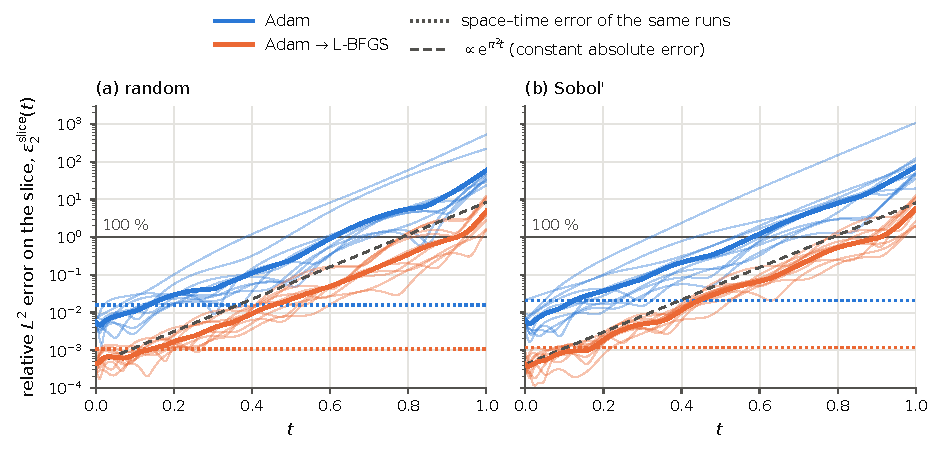
\includegraphics[width=\textwidth]{s4_lowdim_timeslices.pdf}
\caption{Relative $L^2$ error $\errT(t)$ on the time slice $t$ of problem \PH,
evaluated on 201 points in $x$ at each of 201 time levels, for (a)~\strat{random} and
(b)~\strat{Sobol} points, $\Nr=256$, seeds 0 to 9, and the arms \Adam\ (blue) and
\AdamLBFGS\ (orange). Thin lines: single seeds; thick lines: geometric mean over seeds.
Dotted lines: geometric mean of the space--time error $\errL$ of the same runs, in the
colour of the arm. Dashed line: growth proportional to $\ee^{\pi^2t}$, the slice error of
a constant absolute error, drawn through the \AdamLBFGS\ mean at $t=0$. Horizontal line:
100 per cent.}
\label{s4_lowdim:fig:timeslice}
\end{figure}
% src: data/s4_lowdim_timeslices.json -> code/s4_lowdim_timeslices.py plot

% =====================================================================================
% sections/s5_hard.tex -- Section 5.
% Numbers: every quantitative statement is preceded or followed by "% src: <path relative
% to the root of the repository>".  Experiments of this section:
%   longer runs on Wave2   code/s5_hard_wave2d_long.py        -> data/s5_hard_wave2d_long.json
%   Lap3s with control     code/s5_hard_laplace3d_smooth.py   -> data/s5_hard_laplace3d_smooth.json
%   longer runs on Wave1   code/s5_hard_wave1d_long.py        -> data/s5_hard_wave1d_long.json
% Finite differences on Lap3s (no training): code/s5_hard_fd_lap3s.py -> data/s5_hard_fd_lap3s.json
% Plot/table regeneration (no training, no new timing):
%       code/s5_hard_cost.py               -> data/s5_hard_cost.json, figures/s5_hard_cost.pdf
%       code/s5_hard_wave1d_floor.py       -> data/s5_hard_wave1d_floor.json
%       code/s5_hard_tables.py             -> data/s5_hard_tables.tex and the rows between the
%                                             GENERATED markers of the two tables below
% Figures and further details: sections/S4_hard.tex.
% =====================================================================================
\section{Wave equations, the three-dimensional Laplace problem and classical baselines}
\label{s5_hard:sec}

Three of the five low-dimensional problems are not brought to the $10^{-3}$ level of
Section~\ref{s4_lowdim:sec} by the common protocol (unit weights, 1500 \Adam\ and 1500
\LBFGS\ iterations): the two-dimensional wave problem \PWtwo, the three-dimensional Laplace
problem \PLthree\ and the two-mode wave problem \PWone. They fall short for three different
reasons, which this section separates with three further experiments; it then sets all five
problems against second-order finite differences. Table~\ref{s5_hard:tab:hard} collects the
numbers.

\begin{table}[tbp]
\centering
\footnotesize
\setlength{\tabcolsep}{4pt}
\caption{Held-out errors on the three harder problems. Benchmark rows (25 runs: five
strategies, five seeds each): range of the five strategy means, with $[\min,\max]$ over
the 25 single runs underneath.
Other rows: one strategy (\strat{Sobol}), mean $\pm$ sample standard deviation over the
seeds, with $[\min,\max]$ over the seeds underneath. Every row has 3000 iterations per arm
except the two ``long runs'': 1500 \Adam\ iterations followed by
\LBFGS\ until the optimiser stopped (after 8024 to 8437 \LBFGS\ iterations for \PWtwo\
and 7370 to 9224 for \PWone), and 10\,000 (\PWtwo) or 41\,000 (\PWone) \Adam\ iterations
for the \Adam\ column. ``Control'': \PLthree\ re-run with the
driver and device used for \PLthreeS. Evaluation sets as in
Table~\ref{s2_problems:tab:problems}.}
\label{s5_hard:tab:hard}
% src: research_benchmark/results/benchmark_runs.csv (benchmark rows; strategy means as in research_benchmark/results/tables.md T1)
% src: data/s5_hard_wave2d_long.json (Wave2 long run, summary block)
% src: data/s5_hard_laplace3d_smooth.json (Lap3 control and Lap3s)
% src: data/s5_hard_wave1d_long.json (Wave1 long run, summary block)
% rows generated by code/s5_hard_tables.py
\begin{tabular}{@{}llll@{}}
\toprule
Problem, set-up & $\errL$, \Adam & $\errL$, \AdamLBFGS & $\errI$, \AdamLBFGS \\
\midrule
%% BEGIN GENERATED s5_hard:tab:hard
\PWtwo, benchmark & $0.203$--$0.235$ & $\sci{4.79}{-2}$--$\sci{5.01}{-2}$ & $0.078$--$0.081$ \\
\quad 25 runs & $[0.148,\,0.343]$ & $[\sci{2.71}{-2},\,\sci{8.15}{-2}]$ & $[0.050,\,0.121]$ \\[0.3em]
\PWtwo, long run & $(8.80\pm 2.55)\times 10^{-2}$ & $(7.99\pm 2.00)\times 10^{-3}$ & $(1.98\pm 0.33)\times 10^{-2}$ \\
\quad 3 seeds & $[0.065,\,0.115]$ & $[\sci{5.68}{-3},\,\sci{9.31}{-3}]$ & $[\sci{1.74}{-2},\,\sci{2.36}{-2}]$ \\[0.3em]
\PLthree, benchmark & $0.118$--$0.300$ & $\sci{3.56}{-2}$--$\sci{4.88}{-2}$ & $0.070$--$0.101$ \\
\quad 25 runs & $[0.083,\,0.908]$ & $[\sci{3.02}{-2},\,\sci{6.32}{-2}]$ & $[0.059,\,0.231]$ \\[0.3em]
\PLthree, control & $0.135\pm 0.037$ & $(3.72\pm 0.26)\times 10^{-2}$ & $(7.22\pm 1.34)\times 10^{-2}$ \\
\quad 5 seeds & $[0.104,\,0.193]$ & $[\sci{3.36}{-2},\,\sci{4.04}{-2}]$ & $[0.055,\,0.091]$ \\[0.3em]
\PLthreeS & $(3.25\pm 0.56)\times 10^{-2}$ & $(3.32\pm 0.76)\times 10^{-3}$ & $(1.14\pm 0.47)\times 10^{-2}$ \\
\quad 5 seeds & $[\sci{2.77}{-2},\,\sci{4.18}{-2}]$ & $[\sci{2.71}{-3},\,\sci{4.61}{-3}]$ & $[\sci{6.90}{-3},\,\sci{1.81}{-2}]$ \\[0.3em]
\PWone, benchmark & $0.481$--$0.486$ & $0.435$--$0.449$ & $0.652$--$0.690$ \\
\quad 25 runs & $[0.461,\,0.512]$ & $[0.414,\,0.464]$ & $[0.575,\,0.745]$ \\[0.3em]
\PWone, long run & $0.365\pm 0.020$ & $0.365\pm 0.024$ & $0.546\pm 0.012$ \\
\quad 3 seeds & $[0.343,\,0.380]$ & $[0.337,\,0.381]$ & $[0.533,\,0.557]$ \\
%% END GENERATED s5_hard:tab:hard
\bottomrule
\end{tabular}
\end{table}

% -------------------------------------------------------------------------------------
\subsection{The two-dimensional wave problem}
\label{s5_hard:sec:w2}

With the benchmark protocol ($2\times 50$ network, $\Nr=512$, five seeds) the five strategy
means of $\errL$ on \PWtwo\ after \AdamLBFGS\ lie between $\sci{4.79}{-2}$ and
$\sci{5.01}{-2}$, single runs between $\sci{2.7}{-2}$ and $\sci{8.2}{-2}$, and \Adam\ alone
gives strategy means of 0.20 to 0.24.
% src: research_benchmark/results/tables.md (T1, T3); research_benchmark/results/benchmark_runs.csv
No strategy differs from \strat{random} (paired ratios 0.99 to 1.07, all $p\ge 0.8$).
% src: research_benchmark/results/runs/wave2d_s0-5.json; notes/VERIFICATION.md (sec. 2.1: recomputed by the verification)
These are not converged values: the median held-out error of the 25 runs is
$\sci{7.24}{-2}$ after 1000 \LBFGS\ iterations and $\sci{4.58}{-2}$ after 1500, and it is
still falling when the budget ends.

We therefore repeated the \strat{Sobol} configuration for seeds 0, 1 and 2 with a budget of
10\,000 iterations: 1500 \Adam\ iterations followed by up to 8500 \LBFGS\ iterations, and
10\,000 \Adam\ iterations as a comparator (single-network driver, single precision). At
iteration 3000 these runs agree with the benchmark runs of the same seeds (Supplementary
Section~\ref{S4:sec:w2}).
% src: code/s5_hard_wave2d_long.py; data/s5_hard_wave2d_long.json (summary.per_seed: lbfgs_iters, stop, adam_lbfgs_rel_l2, adam_lbfgs_linf); research_benchmark/pinnbench/core.py (run_single: tolerance_grad, tolerance_change)
In all three seeds the \LBFGS\ phase ended before the budget, on the optimiser's own
termination test, after 8024, 8437 and 8345 iterations, with
$\errL=\sci{9.31}{-3}$, $\sci{8.98}{-3}$ and $\sci{5.68}{-3}$ (mean $\sci{7.99}{-3}$,
standard deviation $\sci{2.00}{-3}$) and $\errI$ between $\sci{1.7}{-2}$ and
$\sci{2.4}{-2}$: five to eight times below the error at iteration 3000.
% src: data/s5_hard_wave2d_long.json (adam_lbfgs_test_ratio_9500_over_8500; adam_rel_l2 per seed)
The curves have flattened but are not flat: over the last 1000 logged iterations before
iteration 9500 the error still falls by 8 to 15 per cent. The 0.6 to 0.9 per cent quoted
here is where this optimiser stopped in single precision, not a limit of the method; double
precision, a restarted \LBFGS\ or more collocation points might lower it, and none was
tested. \Adam\ alone is at $\sci{6.5}{-2}$ to 0.115 after 10\,000 iterations and still
descending.
% src: data/s5_hard_wave2d_long.json (runs[*].adam_lbfgs.centre_value; summary.per_seed.max_abs_centre_error)
The learnt function is a standing wave: at $(x,y)=(0.5,0.5)$ it changes sign between
$t=0.35$ and $t=0.40$ (exact zero at $t=1/(2\sqrt2)\approx 0.354$) and ends at $-0.264$,
$-0.263$ and $-0.266$ at $t=1$ (exact $-0.266$); the largest deviation over the 21 times and
three seeds is $\sci{3.2}{-3}$ (Figure~\ref{s5_hard:fig:wave2d}).

% -------------------------------------------------------------------------------------
\subsection{The three-dimensional Laplace problem: dimension or data?}
\label{s5_hard:sec:l3}

For \PLthree\ ($2\times 100$ network, $\Nr=512$, $12\times 12$ points per face) the
strategy means after \AdamLBFGS\ are $\sci{3.56}{-2}$ to $\sci{4.88}{-2}$ (single runs
$\sci{3.0}{-2}$ to $\sci{6.3}{-2}$), with $\errI$ between 0.07 and 0.10.
% src: research_benchmark/results/tables.md (T1); research_benchmark/results/benchmark_runs.csv
The Dirichlet data of \PLthree\ are discontinuous along two edges
(Proposition~\ref{s2_problems:prop:exact}(b)), so no function that is continuous on the
closed cube is uniformly accurate near them. A classical solver is affected too: the
seven-point finite-difference scheme with $n=20$ intervals per side ($21^3$ nodes) has the
same $L^2$ accuracy as the PINN ($\errL=\sci{3.90}{-2}$, with $\errI=0.171$), and $n=40$
($41^3$ nodes) gives $\sci{9.97}{-3}$ and $0.0434$.
% src: research_benchmark/results/classical.json (laplace3d, n = 20, 40); verify_research_benchmark/v_fd.out
% src: data/s5_hard_fd_lap3s.json (ratio_Lap3_over_Lap3s_rel_l2: 18.5, 18.9, 11.6, 12.5 for n = 20, 40, 80, 160), script code/s5_hard_fd_lap3s.py
With the compatible datum of \PLthreeS\ the same scheme is 12 to 19 times more accurate on
every grid tried.

To separate the third dimension from the discontinuity we solved \PLthreeS\ with the network,
\strat{Sobol} points, face points, optimiser settings, seeds (0 to 4) and evaluation grid of
the benchmark, and re-ran \PLthree\ alongside as a control.
% src: code/s5_hard_laplace3d_smooth.py; data/s5_hard_laplace3d_smooth.json (keys L3s = Lap3s, L3 = Lap3; paired_ratio_L3_over_L3s_adam_lbfgs_rel_l2); research_benchmark/results/tables.md (T1, laplace3d sobol)
The control reproduces the benchmark ($\sci{3.72}{-2}\pm\sci{2.6}{-3}$ against
$\sci{3.56}{-2}\pm\sci{3.7}{-3}$). With compatible data the same set-up reaches
$\errL=\sci{3.32}{-3}\pm\sci{7.6}{-4}$ (range $\sci{2.71}{-3}$ to $\sci{4.61}{-3}$) and
$\errI=\sci{1.14}{-2}\pm\sci{4.7}{-3}$: seed by seed, the error on \PLthree\ is 8.8 to 14.1
times larger (geometric mean 11.4, all five seeds).
% src: data/s5_hard_laplace3d_smooth.json (share_sq_error_nearest_5pct_to_singular_edges)
In the \PLthree\ runs the 5 per cent of evaluation points closest to the two singular edges
carry 67 to 79 per cent of the squared error (19 to 35 per cent for \PLthreeS).
The several-per-cent error on \PLthree\ is therefore mainly a property of the data, not of
the dimension (the data of \PLthreeS\ are compatible and also make the solution a single
separable mode, so the comparison does not separate these two changes): with $\Nr=512$ points
and 3000 iterations a three-dimensional harmonic function with compatible data is recovered
to 0.3 per cent.
% src: data/s5_hard_laplace3d_smooth.json (Lap3s rows under the key L3s, curve at iterations 2750 and 3000); data/s5_hard_fd_lap3s.json
That figure is not converged either (the median error falls from $\sci{4.1}{-3}$ to
$\sci{3.1}{-3}$ over the last 250 iterations), and the conclusion rests on one strategy and
five seeds. The PINN's factor between \PLthree\ and \PLthreeS\ (geometric mean 11.4) is close
to that of the finite-difference scheme, 12 on the grids on which the evaluation points are
nodes.

% -------------------------------------------------------------------------------------
\subsection{The two-mode wave problem}
\label{s5_hard:sec:w1}

Problem \PWone\ is not solved by the benchmark protocol. All 50 runs ($3\times 64$
network, $\Nr=1024$; 25 networks, two arms) end between 0.414 and 0.512 (\Adam\ 0.461 to
0.512, \AdamLBFGS\ 0.414 to 0.464). No strategy moves the error by more than 2 per cent
(paired ratios to \strat{random} 0.98 to 1.02).
% src: research_benchmark/results/benchmark_runs.csv; research_benchmark/results/tables.md (T2, T3); verify_research_benchmark/v_stats.out
% src: code/s5_hard_wave1d_floor.py; data/s5_hard_wave1d_floor.json
A predictor that reproduces the slow mode $\sin\pi x\cos 2\pi t$ and omits the fast one has
$\errL=1/\sqrt5\approx 0.447$ (the two modes are orthogonal with squared norms $1/4$ and
$1/16$), and this is close to what the networks do: projected onto the two spatial modes,
the stored predictions of seed 0 reproduce the slow mode to within 4 to 12 per cent, and the
fast mode carries 84 to 93 per cent of the squared error (Supplementary
Section~\ref{S4:sec:w1}).
% src: data/s5_hard_wave1d_long.json (summary.benchmark_seed0: share_sq_error_mode4 0.89 to 0.93 and 0.84 to 0.89; rel_l2_a1 0.078 to 0.117 and 0.036 to 0.092)

% src: refs.bib (wangyu2022 and rathore2024, annotations); data/checks/verification.json (literature_wave1: arXiv:2007.14527, Sec. 7.3 and caption of Fig. 6)
Two published results bracket this outcome, and neither is a like-for-like comparison.
\citet{wangyu2022}, who introduced the problem, report $\sci{4.518}{-1}$ for the
unweighted PINN trained with a first-order optimiser (five layers of 500 units, 80\,000
iterations) and $\sci{1.728}{-3}$ with weights derived from the neural tangent kernel.
\citet{rathore2024} train the unweighted loss on the same equation with a faster second
mode ($\sin5\pi x$ in place of $\sin4\pi x$), three hidden layers of 50 to 400 units,
10\,000 residual points and 41\,000 iterations: the run with the lowest loss after tuning reaches 0.349 with
\Adam, 0.335 with \LBFGS, 0.055 with \Adam\ followed by \LBFGS\ (their Table~1) and 0.013
after a further Newton--conjugate-gradient phase (their Table~2). The unweighted loss can
therefore be brought to a few per cent, and the level 0.41 to 0.51 of our benchmark is
not a limit of the formulation.

% src: code/s5_hard_wave1d_long.py; data/s5_hard_wave1d_long.json (summary.per_seed: adam_rel_l2 0.371, 0.343, 0.380; adam_lbfgs_rel_l2 0.376, 0.337, 0.381; lbfgs_iters 8310, 9224, 7370; stop converged_tolerance; adam_lbfgs_final_loss 0.0247, 0.0199, 0.0269)
Whether the budget alone is responsible was tested by repeating the \strat{Sobol}
configuration for seeds 0, 1 and 2 with their budget of 41\,000 iterations (single-network
driver, single precision): 41\,000 \Adam\ iterations in one arm, and 1500 \Adam\ iterations
followed by \LBFGS\ in the other (Table~\ref{s5_hard:tab:hard}). The budget does not rescue
the problem at this network size. \Adam\ ends at 0.371, 0.343 and 0.380 and is still
descending slowly. The \LBFGS\ phase stops on its own termination test after 8310, 9224 and
7370 iterations, at 0.376, 0.337 and 0.381, with a loss of 0.020 to 0.027, which is 0.16 to
0.19 of its value at the switch and far from zero; \citet{rathore2024} describe the same
behaviour of \LBFGS, which in their runs stops before the iteration limit without reaching a
critical point.
% src: data/s5_hard_wave1d_long.json (summary.per_seed[*].adam_lbfgs_modes and adam_modes: rel_l2_a1 0.004 to 0.019; rel_l2_a4 0.71 to 0.83; share_sq_error_mode4 0.89 to 0.94)
In these six runs the slow mode is accurate to 0.4 to 1.9 per cent, the amplitude of the fast
mode is in error by 71 to 83 per cent, and the fast mode carries 89 to 94 per cent of the
squared error: the fast oscillation is followed over its first period and then dies out,
although the exact amplitude is constant (Figure~\ref{s5_hard:fig:wave1d}).

The statement supported by our runs is therefore narrow: with three hidden layers of 64
units, 1024 residual points, unit weights and single precision, neither 41\,000 \Adam\
iterations nor an \LBFGS\ phase run to its termination resolves the fast mode.
% src: refs.bib (rathore2024, annote: Sec. 2.2, widths, residual points, L-BFGS memory 100, tuned Adam rate, switch after 1000, 11000 or 31000 Adam iterations); research_benchmark/pinnbench/core.py (LBFGS_MEMORY = 50)
The runs of \citet{rathore2024} differ from ours in the width of the network (up to 400), the
number of residual points (ten times as many), the memory of \LBFGS\ (100 against 50), a tuned
\Adam\ rate and switch point, the initialisation and the selection of the best run; which of
these matters was not tested, nor was double precision. None of the remedies proposed in the
literature was tried either (Section~\ref{s8_discussion:sec:nottried}).

% -------------------------------------------------------------------------------------
\subsection{Finite-difference baselines and cost}
\label{s5_hard:sec:fd}

\begin{table}[tbp]
\centering
\footnotesize
\setlength{\tabcolsep}{2.6pt}
\caption{PINN against second-order finite differences (FD). ``PINN $\errL$'': lowest
geometric mean over seeds among the five strategies, \AdamLBFGS\ arm, 3000 iterations.
FD columns: the coarsest grid of the refinement sequence whose $\errL$ on the same held-out
set is at most that value ($n$ intervals per space direction), its errors and its solve
time (best of three). $t_{\mathrm{PINN}}$: time of one \AdamLBFGS\ run in the three
measurements A, B and C described under ``Cost'' in the text; ranges are over runs (B)
or stacks (C). Ratio: $t_{\mathrm{PINN}}/t_{\mathrm{FD}}$ for B and for C.}
\label{s5_hard:tab:fd}
% src: data/s5_hard_cost.json (built by code/s5_hard_cost.py from the files below)
% src: research_benchmark/results/classical.json; research_benchmark/results/benchmark_runs.csv
% src: research_benchmark/results/runs/*_s*-*.json (C: timing.t_adam_to_branch, t_lbfgs_total, batch_size)
% src: research_benchmark/results/timing_single.json (A); verify_research_benchmark/v_runs.json, v_runs_extra.json (B; printed in v_summary.out)
% rows generated by code/s5_hard_tables.py
\resizebox{\textwidth}{!}{%
\begin{tabular}{@{}llrlllrrrll@{}}
\toprule
 & PINN $\errL$ & \multicolumn{4}{c}{finite differences} & \multicolumn{3}{c}{$t_{\mathrm{PINN}}$ (s)} & \multicolumn{2}{c}{ratio} \\
\cmidrule(lr){3-6}\cmidrule(lr){7-9}\cmidrule(l){10-11}
 & (strategy) & $n$ & $\errL$ & $\errI$ & $t_{\mathrm{FD}}$ (s) & (A) & (B) & (C) & B & C \\
\midrule
%% BEGIN GENERATED s5_hard:tab:fd
\PH & $\sci{1.07}{-3}$ (\strat{RAD}) & 100 & $\sci{5.05}{-4}$ & $\sci{2.71}{-4}$ & $\sci{2.2}{-3}$ & 216 & 20--37 & 12 & $(0.9$--$1.7)\times 10^{4}$ & $\sci{5.6}{3}$ \\
\PLtwo & $\sci{2.28}{-4}$ (\strat{grid-c}) & 100 & $\sci{7.51}{-5}$ & $\sci{6.22}{-5}$ & $\sci{2.4}{-2}$ & 402 & 46--83 & 12--14 & $(1.9$--$3.4)\times 10^{3}$ & $(4.8$--$5.7)\times 10^{2}$ \\
\PWone & $0.435$ (\strat{grid-c}) & 25 & $\sci{5.14}{-2}$ & $\sci{9.45}{-2}$ & $\sci{4.4}{-4}$ & 302 & 60 & 7 & $\sci{1.3}{5}$ & $\sci{1.5}{4}$ \\
\PWtwo & $\sci{4.61}{-2}$ (\strat{Sobol}) & 20 & $\sci{5.12}{-3}$ & $\sci{8.83}{-3}$ & $\sci{3.5}{-4}$ & 273 & 36 & 7 & $\sci{1.0}{5}$ & $\sci{2.1}{4}$ \\
\PLthree & $\sci{3.55}{-2}$ (\strat{Sobol}) & 40 & $\sci{9.97}{-3}$ & $\sci{4.34}{-2}$ & $\sci{1.6}{-3}$ & 341 & 50 & 12 & $\sci{3.1}{4}$ & $\sci{7.3}{3}$ \\
%% END GENERATED s5_hard:tab:fd
\bottomrule
\end{tabular}%
}
\end{table}

The finite-difference baselines of Section~\ref{s3_methods:sec:fd} were run on sequences of
grids and evaluated on the held-out sets used for the PINNs.
Table~\ref{s5_hard:tab:fd} lists, for each problem, the coarsest grid that is at least as
accurate as the best PINN geometric mean: $n=100$ for \PH\ and \PLtwo, and the coarsest or
second-coarsest grid tried for the other three.
% src: data/s5_hard_cost.json (summary.fd_error_over_pinn_error_range: 0.111 to 0.470)
The accuracies are not equal: the grid listed has between 0.11 and 0.47 times the error of
the PINN, so the comparison is at equal or better accuracy of the finite-difference
solve.
% src: research_benchmark/results/classical.csv (wave1d, n = 25: rel_l2 0.05140); research_benchmark/results/benchmark_runs.csv (wave1d, best run 0.414); data/s5_hard_wave1d_long.json (best long run 0.3367, seed 1, adam_lbfgs)
On \PWone\ the coarsest grid is eight times more accurate than any benchmark run (6.6 times
more accurate than the best of the longer runs), and on \PWtwo\ even the long runs of
Section~\ref{s5_hard:sec:w2} ($\sci{5.7}{-3}$ to $\sci{9.3}{-3}$) stay above the
$\sci{5.12}{-3}$ of the $n=20$ grid.
% src: data/s5_hard_cost.json; research_benchmark/results/classical.json; data/s5_hard_wave2d_long.json; research_benchmark/results/classical.csv (observed_order_rel_l2)
The observed order of convergence is 1.99 to 2.01 in all 18 refinements on \PH, \PWone,
\PWtwo\ and \PLtwo; on \PLthree\ it is 1.97, 2.70 and 1.89, and with the compatible datum of
\PLthreeS\ it is 1.99, 2.00 and 2.00 (Table~\ref{sC_details:tab:fdconv} and Supplementary
Section~\ref{S4:sec:fd}).

\paragraph{Cost.}
The finite-difference solves of Table~\ref{s5_hard:tab:fd} take $\sci{3.5}{-4}$ to
$\sci{2.4}{-2}$~s.
% src: research_benchmark/results/classical.json
For the PINN we have three measurements, all on the same shared 12-core machine and none
on an idle one; they differ in the driver as well as in the load
(Supplementary Section~\ref{S4:sec:cost}).
% src: research_benchmark/results/timing_single.json; verify_research_benchmark/v_runs.json; verify_research_benchmark/v_runs_extra.json; research_benchmark/results/runs/*_s*-*.json (timing)
(A)~Single networks on the CPU, timed for 400 \Adam\ and 200 \LBFGS\ iterations under heavy
load and extrapolated to 3000 iterations: 216 to 402~s. (B)~Single networks on the CPU, the
runs of \textsf{V-bench} at a load average of about 20 to 45: 20 to 83~s. (C)~The stacked GPU
driver that produced the errors of the benchmark, per network of a stack of 25 or 50: 6.9 to
13.9~s; this amortised time is reached only when that many networks are trained at once.
% src: data/s5_hard_cost.json (summary: ratio_C_range 4.76e2 to 2.08e4, ratio_B_range 1.91e3 to 1.34e5, ratio_A_range 1.66e4 to 7.70e5, A_over_B_median_range 5.1 to 8.3, ratio_smallest_of_all_measurements 475.6); data/sC_details_numbers.json (cost: median of run_B_s over run_C_s 2.1 to 8.7 per problem)
Measurement A is 5.1 to 8.3 times the median of B, and the median of B 2.1 to 8.7 times C, so
only orders of magnitude are meaningful. One PINN run costs $\sci{1.9}{3}$ to $\sci{1.3}{5}$
times the finite-difference solve that is at least as accurate when a single network is
trained (B): three to five orders of magnitude. Per network of a GPU stack (C) the ratio is
$\sci{4.8}{2}$ to $\sci{2.1}{4}$, and with A it is $\sci{1.7}{4}$ to $\sci{7.7}{5}$, which is
inflated by the load. The smallest ratio in any measurement is $\sci{4.8}{2}$ (\PLtwo, C)
(Figure~\ref{s5_hard:fig:cost}). The finite-difference times are the best of three
solves, the PINN times single measurements; no timing is taken from the longer runs or the
control experiments.

This is the expected outcome for linear problems on boxes in one to three dimensions and
agrees with the systematic comparison of \citet{grossmann2024} with finite elements. It
also illustrates why a classical baseline belongs in every such study
\citep{mcgreivy2024}. What it does not address are the settings usually put forward for
PINNs---irregular geometry, inverse problems, high dimension---of which only the last is
examined in this article (Section~\ref{s6_highdim:sec}).

% =====================================================================================
% sections/s6_highdim.tex -- Dimension scaling: PINN versus Deep Ritz for d = 2 to 20.
%
% Every number below is recomputed from the stored per-run records by
%   code/s6_highdim_tables.py  -> data/s6_highdim_numbers.json, data/s6_highdim_tables.tex
% Figures: code/s6_highdim_figs.py (plot-only).
% 16 000 iterations at d = 20: code/s6_highdim_long_d20.py -> data/s6_highdim_long_d20.jsonl.
% Diagnostics of the d = 20 networks: code/s6_highdim_diag.py -> data/s6_highdim_diag_d20.json.
% Sections 6.7 and 6.8: code/s6_highdim_bound.py and code/s6_highdim_remedies.py
%   -> data/s6_highdim_bound_{numbers.json,tables.tex}, data/s6_highdim_remedies_{recheck.json,tables.tex},
%   figures/s6_bound.pdf, figures/s6_remedies_{ratios,altridge}.pdf, from the result files of
%   research_highdim_bound/ and research_highdim_remedies/ (no training).
% Table rows between GENERATED markers are written by these scripts (code/inject.py finds the
% marker in any section file).  Further results, tables and figures: sections/S5_highdim.tex.
% =====================================================================================
\section{Dimension scaling: PINN versus Deep Ritz for \texorpdfstring{$d=2$}{d = 2} to 20}%
\label{s6_highdim:sec}

Neural solvers are usually motivated by problems in many dimensions, where a mesh is out
of reach~\citep{eyu2018,sirignano2018,han2018}. This section measures how the accuracy and
the cost of the PINN and of the Deep Ritz method change with the dimension, on the Laplace
problem \Pone~\eqref{s2_problems:eq:p1} and the Poisson problem \Ptwo~\eqref{s2_problems:eq:p2}
for $d=2,3,5,10,20$, with the protocol of Section~\ref{s3_methods:sec:highdim}: one network
($d$--64--64--64--1, tanh), 1024 interior and 1024 boundary points redrawn at every
iteration, \Adam\ with two learning-rate reductions, 4000 iterations unless stated,
$\lam=1000$ for the PINN, $\bet=100$ (\Pone) and $\bet=1$ (\Ptwo) for Deep Ritz, and the
error of the final network on 50\,000 held-out points. Each cell has three seeds (0, 1, 2).
% src: research_highdim/scripts/hd_core.py (train: torch.manual_seed(seed), generator 1000+seed for both methods)
Within a seed the two methods start from the same weights and see the same points, so the
comparison is paired. One fact frames the results: \Ptwo\ has $\dn\uex=0$ and is the best
case for the penalised energy, which is then unbiased, whereas \Pone\ is the generic,
biased case (Proposition~\ref{s3_methods:prop:robin}); the PINN loss has no such bias
(Remark~\ref{s3_methods:rem:consistent}). Sections~\ref{s6_highdim:sec:equal-its}
to~\ref{s6_highdim:sec:weights} report the comparison. Section~\ref{s6_highdim:sec:bound} then
proves an explicit stability constant for the unit cube, which turns the two terms of the PINN
loss into a computable bound on the error of any network, and Section~\ref{s6_highdim:sec:remedies}
tests two cheap remedies for the plateau that both methods reach on \Ptwo\ at $d=20$.

% -------------------------------------------------------------------------------------
\subsection{Accuracy at equal iterations}\label{s6_highdim:sec:equal-its}

\begin{figure}[tbp]
\centering
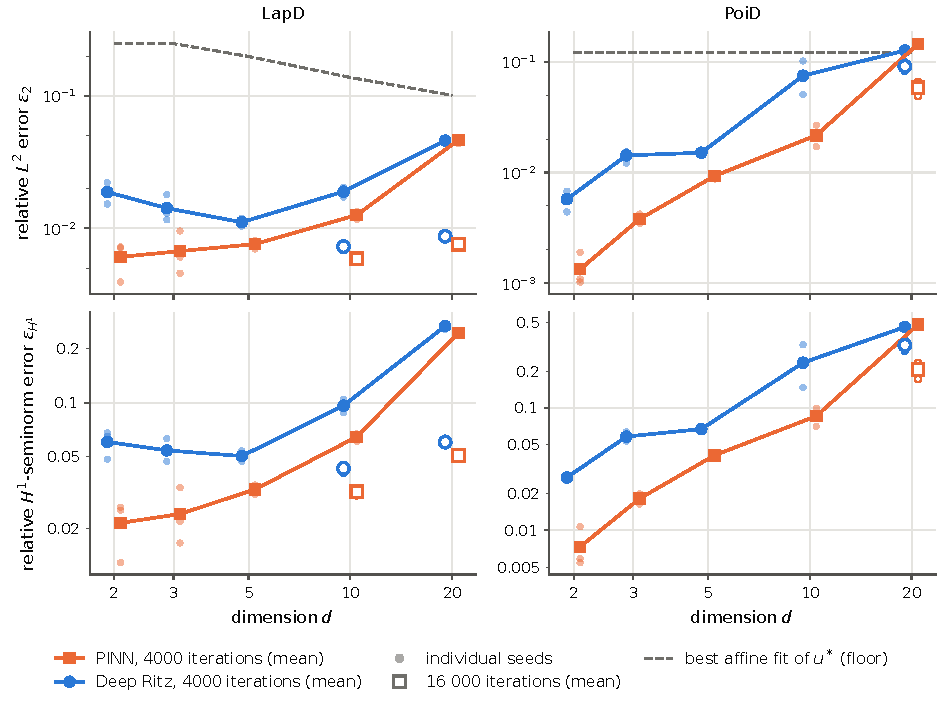
\includegraphics[width=0.8\textwidth]{s6_highdim_error.pdf}
\caption{Held-out errors against the dimension for \Pone\ (left) and \Ptwo\ (right):
relative $L^2$ error $\errL$ (top) and relative $H^1$-seminorm error $\errH$ (bottom) on
50\,000 test points. Filled symbols joined by lines: mean over seeds 0--2 after 4000
iterations (the values of Tables~\ref{s6_highdim:tab:p1} and~\ref{s6_highdim:tab:p2});
small dots: the individual seeds. Open symbols: the same after 16\,000 iterations, run for
\Pone\ at $d=10$ and for both problems at $d=20$. Dashed line: $\errL$ of the best affine
approximation of $\uex$ (Proposition~\ref{s2_problems:prop:floors}). PINN in orange
(squares), Deep Ritz in blue (circles); the two methods are offset horizontally for
legibility.}
\label{s6_highdim:fig:error}
% src: research_highdim/results/runs*.jsonl; data/s6_highdim_long_d20.jsonl; data/closed_forms.json; script code/s6_highdim_figs.py
\end{figure}

% src: research_highdim/results/summary.csv; research_highdim/results/derived.txt (ratios, range overlap; boundary vs interior)
For every $d\le10$ the PINN is the more accurate method on both problems
(Tables~\ref{s6_highdim:tab:p1} and~\ref{s6_highdim:tab:p2},
Figure~\ref{s6_highdim:fig:error}): the ratio of the mean errors lies between 1.46 and 4.29,
and in each of the eight cells the three PINN seeds are below the three Deep Ritz seeds. The
$H^1$-seminorm errors are ordered in the same way. At $d=20$ the two methods are level on
\Pone\ (ratio 0.99, overlapping ranges) and Deep Ritz is 12 per cent lower on \Ptwo. In every
cell the relative $L^2$ error on 20\,000 held-out boundary points is between 0.65 and 2.11
times the interior error.
% src: verify_research_highdim/results/v_summary.txt (rows 'main'); data/s6_highdim_numbers.json (vdim_main, vdim_P1_d20_ritz_sd_5_seeds = 4.06e-3)
The verification code \textsf{V-dim} confirms the ordering: at $d=2$ and $d=10$, on both
problems, each of its PINN seeds is below each of its Deep Ritz seeds
(Table~\ref{s6_highdim:tab:vdim}). It also shows that three seeds understate the spread (on
\Pone\ at $d=20$ its five Deep Ritz seeds have a standard deviation of $\sci{4.1}{-3}$ against
$\sci{1.8}{-3}$ for our three), so we rely only on differences that hold for every seed.

% -------------------------------------------------------------------------------------
\subsection{Growth with the dimension, and trivial-predictor floors}\label{s6_highdim:sec:growth}

% src: research_highdim/results/derived.txt (log-log slopes of the geometric-mean error); recomputed in data/s6_highdim_numbers.json (slopes_geomean); research_highdim/results/summary.csv (laplace, ritz: rel_l2_mean 1.8821e-2, 1.4214e-2, 1.1126e-2, 1.8964e-2 at d = 2, 3, 5, 10)
At this fixed budget the error grows with $d$ for both methods, except Deep Ritz on \Pone\ for
$d\le10$, where it is not monotone ($\sci{1.88}{-2}$, $\sci{1.42}{-2}$, $\sci{1.11}{-2}$ and
$\sci{1.90}{-2}$ at $d=2$, 3, 5 and 10). A least-squares line through
the logarithm of the geometric-mean error against $\log d$ over $d=2,\dots,10$ has slope 0.48
(PINN) and 0.01 (Deep Ritz) on \Pone, and 1.71 and 1.46 on \Ptwo; with $d=20$ included the
slopes are 0.86, 0.41, 1.92 and 1.35. These numbers describe one budget and four or five
dimensions. They are not rates: Section~\ref{s6_highdim:sec:budget} shows that they change
with the budget.
% src: data/closed_forms.json (floors); research_highdim/results/summary.csv (rel_l2_centered_mean)
Relative errors must be read against the floors of Proposition~\ref{s2_problems:prop:floors}.
The solution of \Pone\ concentrates around its mean as $d$ grows, so both floors fall with $d$
and plain $\errL$ flatters \Pone\ in high dimension: the centred error of the PINN rises from
$\sci{9.2}{-3}$ at $d=2$ to $\sci{3.4}{-2}$ at $d=10$ and $\sci{1.73}{-1}$ at $d=20$, so the
``4.7 per cent'' of Table~\ref{s6_highdim:tab:p1} at $d=20$ is 17 per cent of the fluctuation
of $\uex$. For \Ptwo\ the affine floor is $0.1203$ in every dimension, and at $d=20$ both
methods end above it ($0.144$ and $0.126$): after 4000 iterations neither improves on the
best affine function.

% -------------------------------------------------------------------------------------
\subsection{The networks at \texorpdfstring{$d=20$}{d = 20}, and the effect of the budget}%
\label{s6_highdim:sec:budget}

% src: verify_research_highdim/results/v_affine.txt; verify_research_highdim/results/v_resid.txt (the 4000-iteration networks, three seeds each); data/s6_highdim_diag_d20.json (re-computation on other points: 0.18-0.20, 0.90; 0.82-0.83, 0.13-0.16, 0.35-0.36)
The two methods are above the affine floor on \Ptwo\ at $d=20$ for different reasons. Split a
function into its least-squares affine fit and a remainder. For the Deep Ritz networks the
remainder has 0.18 to 0.20 times the norm of the remainder of $\uex$, and the residual
$\norm{\lap\unet+f}/\norm{f}$ is 0.90: these networks are still essentially affine. The PINN
networks are not. Their residual is 0.35 to 0.37, and their remainder has 0.83 to 0.84 times
the right norm, but its correlation with the remainder of $\uex$ is only 0.14 to 0.16: the
PINN has built curvature of the right size and the wrong shape. The following elementary
bound says where its error sits.

\begin{remark}\label{s6_highdim:rem:split}
Let $v\in C^2(\overline{\Om})$, $\Om=(0,1)^d$, $e=v-\uex$ and $r=\lap v+f=\lap e$. Let
$e_0\in H^1_0(\Om)$ be the weak solution of $\lap e_0=r$; then $e-e_0$ is harmonic and has
the boundary values of $e$. Expanding $e_0$ and $r$ in the orthonormal Dirichlet
eigenfunctions $\prod_{i}\sqrt2\sin(k_i\pi x_i)$ of $-\lap$, whose eigenvalues
$\pi^2\sum_i k_i^2$ are at least $d\pi^2$, gives
$\norm{e_0}_{L^2(\Om)}\le\norm{r}_{L^2(\Om)}/(d\pi^2)$. For \Ptwo, where
$\norm{f}=\pi^2\norm{\uex}$, this reads
$\norm{e_0}/\norm{\uex}\le d^{-1}\norm{\lap v+f}/\norm{f}$.
\end{remark}

\noindent
% src: data/s6_highdim_numbers.json (e0_bound_P2_d20); research_highdim/results/summary.csv (bd_rel_l2_mean at d = 20: 0.158, 0.133)
With the measured residuals, the part of the error that the interior residual accounts for is
at most $0.37/20<0.02$ of $\norm{\uex}$ for the PINN and $0.90/20=0.045$ for Deep Ritz, out of
total errors of $0.144$ and $0.126$. For both methods the error is thus mostly a harmonic
function fixed by the mismatch on the boundary, which is 16 per cent (PINN) and 13 per cent
(Deep Ritz) in relative $L^2$ norm. Corollary~\ref{s6_highdim:cor:bound}(c) completes this
remark with an explicit constant for the harmonic part.

\begin{table}[tbp]
\centering
\caption{Effect of the budget: $\errL$ in units of $10^{-2}$, mean $\pm$ sample standard
deviation over seeds 0--2. ``16\,000'' is the same protocol with four times as many
iterations (learning-rate reductions at 8000 and 12\,000). ``Equal compute'' is Deep Ritz
with the number of iterations given in brackets, chosen to match the compute of the
4000-iteration PINN run (Section~\ref{s6_highdim:sec:compute}). Last column: affine floor.
A dash means not run.}
\label{s6_highdim:tab:budget}
\small
\setlength{\tabcolsep}{4pt}
% src: research_highdim/results/summary.csv (4000); research_highdim/results/extensions.json (d = 10: 16 000 and equal compute)
% src: data/s6_highdim_long_d20.jsonl (d = 20: 16 000; script code/s6_highdim_long_d20.py)
% generated by code/s6_highdim_tables.py -> data/s6_highdim_tables.tex
\begin{tabular}{@{}lr cc cc c c@{}}
\toprule
 & & \multicolumn{2}{c}{4000 iterations} & \multicolumn{2}{c}{16\,000 iterations} & equal compute & \\
\cmidrule(lr){3-4}\cmidrule(lr){5-6}\cmidrule(lr){7-7}
 & $d$ & PINN & Deep Ritz & PINN & Deep Ritz & Deep Ritz & floor\\
\midrule
\Pone & 10 & $1.260\pm0.084$ & $1.896\pm0.159$ & $0.588\pm0.027$ & $0.728\pm0.039$ & $0.934\pm0.047$ (10\,000) & 13.9 \\
\Ptwo & 10 & $2.168\pm0.482$ & $7.488\pm2.553$ & -- & -- & $1.376\pm0.111$ (9000) & 12.0 \\
\Pone & 20 & $4.663\pm0.248$ & $4.613\pm0.178$ & $0.757\pm0.023$ & $0.870\pm0.038$ & -- & 10.2 \\
\Ptwo & 20 & $14.424\pm0.176$ & $12.633\pm0.022$ & $5.832\pm0.858$ & $9.102\pm0.808$ & -- & 12.0 \\
\bottomrule
\end{tabular}
\end{table}

% src: research_highdim/results/derived.txt (plateau block); data/s6_highdim_numbers.json (plateau_val_mean)
The validation curves (Figure~\ref{s6_highdim:fig:curves}) show that these errors are limited
by the budget. Within 250 iterations the error falls to about the affine floor; it then stalls
before descending, and the stall lengthens with $d$; at $d=20$ neither method has left the
plateau on \Ptwo\ when the 4000-iteration run ends. That networks fit the smoothest component
first is a known tendency~\citep{rahaman2019}; we cite it as context, not as an explanation.
% src: research_highdim/results/extensions.json (d = 10); data/s6_highdim_long_d20.jsonl, data/s6_highdim_numbers.json (extensions, budget_ratios, growth_P1_d10_to_d20)
With four times the budget (Table~\ref{s6_highdim:tab:budget}) the errors at $d=10$ on \Pone\
fall by a factor 2.1 (PINN) and 2.6 (Deep Ritz), and at $d=20$ on \Pone\ by a factor 6.2 and
5.3. On \Ptwo\ at $d=20$ both methods leave the plateau and all six runs end below the affine
floor: $\sci{5.83}{-2}$ for the PINN and $\sci{9.10}{-2}$ for Deep Ritz. These runs are not
converged either: the error is still falling when the learning rate is reduced. With the larger
budget the PINN is again the more accurate method in every seed at $d=20$ (ratio 1.15 on
\Pone, 1.56 on \Ptwo), so the level or reversed ranking after 4000 iterations was an effect of
the budget and, at least in part, of the uncentred input:
% src: research_highdim_remedies/results/summary_exploratory.json (P1/d20/pinn/lift1/4000: 0.0219 to 0.0317; P1/d20/ritz/lift1/4000: 0.0442 to 0.0551)
with the input centred, the PINN is the more accurate method on \Pone\ at $d=20$ after 4000
iterations as well, in every seed (Section~\ref{s6_highdim:sec:remedies}). Much of the growth with
$d$ was also an effect of the budget: from $d=10$ to $d=20$ the PINN error on \Pone\
grows by a factor 3.7 after 4000 iterations and 1.3 after 16\,000 (Deep Ritz: 2.4 and 1.2).
For \Pone, Table~\ref{s6_highdim:tab:p1} is therefore to be read as ``the number of iterations
needed for a given accuracy grows with $d$''. For \Ptwo\ the corresponding long run at $d=10$
was not made, and for neither problem was the approximation power of the network tested
separately.

% -------------------------------------------------------------------------------------
\subsection{Cost per iteration}\label{s6_highdim:sec:cost}

Deep Ritz needs only $\grad\unet$, one reverse pass whatever the dimension. The PINN needs
$\lap\unet$, that is $d$ second derivatives, either by one further reverse pass per coordinate
or by the forward propagation of Section~\ref{s3_methods:sec:highdim}, which evaluates the same
loss. Two separate measurements on the same shared machine (Table~\ref{s6_highdim:tab:cost},
Figure~\ref{s6_highdim:fig:cost}) agree in the following.
% src: data/s6_highdim_numbers.json (cost_growth_d2_to_d100, nested_over_fwd_d_ge_10, cost_primary, cost_verifier); research_highdim/results/cost_vs_d.csv; verify_research_highdim/results/v_bench.txt
From $d=2$ to $d=100$ the cost of a Deep Ritz iteration grows by a factor 1.98 or 1.55, from
3.3 to 5.1\,ms in the quieter measurement, and that of a PINN iteration roughly linearly, as is
known~\citep{hu2024}: by a factor 13.9 or 12.7 (forward Laplacian) and 32.5 or 26.2 (nested).
At $d=100$ a PINN iteration costs about 11 to 13 times a Deep Ritz iteration with the forward
Laplacian and about 29 to 32 times with the nested one; for $d\ge10$ the forward Laplacian is
1.8 to 2.9 times cheaper than the nested one. The milliseconds themselves depend on the load
and are not portable.

% -------------------------------------------------------------------------------------
\subsection{Accuracy at equal compute}\label{s6_highdim:sec:compute}

Because a Deep Ritz iteration is cheaper, a comparison at equal iterations understates the
method. Deep Ritz was therefore also run with the compute of the 4000-iteration PINN run
at $d=10$.
% src: research_highdim/scripts/run_study.py (phase ext, rule); data/s6_highdim_numbers.json (equal_compute_rule: 9594 -> 10000, 8889 -> 9000)
The number of iterations was fixed before the runs, as the mean CPU time of the three PINN runs
divided by the mean CPU time per iteration of the three Deep Ritz runs, rounded to a thousand:
10\,000 on \Pone\ and 9000 on \Ptwo, that is 2.5 and 2.25 Deep Ritz iterations for one PINN
iteration (the cost ratio measured at $d=10$ is 2.23 and 2.48 in the two measurements).
% src: research_highdim/results/extensions.json (phase equaltime); research_highdim/results/summary.csv; data/s6_highdim_numbers.json (equal_compute_gain); verify_research_highdim/results/v_summary.txt (rows 'equaltime', 'eq9k'); notes/VERIFICATION.md (sec. 3.1, V10; sec. 3.3, item 5)
The ranking reverses (Table~\ref{s6_highdim:tab:budget}): Deep Ritz reaches
$\sci{9.34}{-3}\pm\sci{4.7}{-4}$ against $\sci{1.26}{-2}\pm\sci{8.4}{-4}$ for the PINN on
\Pone, and $\sci{1.38}{-2}\pm\sci{1.1}{-3}$ against $\sci{2.17}{-2}\pm\sci{4.8}{-3}$ on \Ptwo,
with disjoint seed ranges in both cases. \textsf{V-dim} agrees (seeds 7--9:
$\sci{8.74}{-3}$, $\sci{9.09}{-3}$, $\sci{9.02}{-3}$ on \Pone; $\sci{1.38}{-2}$,
$\sci{1.24}{-2}$, $\sci{1.50}{-2}$ on \Ptwo). In the re-check of
Section~\ref{s6_highdim:sec:bound}, with a separately written trainer and three seeds, Deep Ritz
at the CPU time of the PINN was also the more accurate on \Pone\ at $d=20$ (descriptive).
% src: data/s6_highdim_bound_numbers.json (recheck_r2: P1_ritz_eqcpu_d20 rel_err 0.0092-0.0104, P1_pinn_d20 0.0459-0.0484)
The ranking of the two methods thus depends on whether iterations or compute are counted. It
does not show that Deep Ritz is the better method: at 16\,000 iterations each the PINN is ahead
at $d=10$ on \Pone\ and at $d=20$ on both problems, although on \Pone\ that lead is of the size
of the penalty bias of Deep Ritz (Section~\ref{s6_highdim:sec:weights}).

% -------------------------------------------------------------------------------------
\subsection{Sensitivity to the penalty weights, and the penalty bias}\label{s6_highdim:sec:weights}

% src: research_highdim/results/sweep.csv (val_rel_l2; d = 5, seed 100); data/s6_highdim_robin_bias.json (weight_sweep_d5: bias 0.1640, 0.02645, 2.991e-3, 3.047e-4; trained_over_bias 0.98, 0.88, 3.44, 36.0)
The weights were selected at $d=5$ from one run per value (Table~\ref{s6_highdim:tab:sweep}).
On \Pone\ the error of Deep Ritz falls by a factor 16 from $\bet=1$ to $\bet=100$ and is level
beyond; the computed penalty bias at $d=5$ explains the first part (it is 0.164 for $\bet=1$
and $\sci{2.64}{-2}$ for $\bet=10$, and these two runs end at 0.98 and 0.88 times it), while
for $\bet=100$ and $1000$ the runs end 3.4 and 36 times above the bias, at an error limited by
the optimisation. On \Ptwo, Deep Ritz is flat, as expected from $\dn\uex=0$, and the PINN needs
$\lam\ge10$.
% src: verify_research_highdim/results/v_summary.txt (rows 'beta', 'lam1e4', 'main' at d = 10); notes/VERIFICATION.md (sec. 3.3, item 3: V11, V13)
These are statements about $d=5$. At $d=10$ larger weights than the chosen ones do not help:
on \Ptwo\ (\textsf{V-dim}, seeds 7--9) Deep Ritz with $\bet=10$ or $100$ and the PINN with
$\lam=10^4$ stay on the affine plateau for the whole run (Supplementary
Section~\ref{S5:sec:weights}).

% src: data/s6_highdim_robin_bias.json (series: beta = 100; against_trained_networks); research_highdim_bound/results/bias_table.json (exact_over_article_series 0.99957 to 1.00026)
The penalty bias of Deep Ritz on \Pone\ was computed for every $d$ of the study by a series in
the Robin eigenfunctions and, exactly, up to $d=100$ by the representation of
Proposition~\ref{sA_proofs:prop:exact};
the two agree to $\sci{4.3}{-4}$ relative (Supplementary Section~\ref{S5:sec:bias} and
Table~\ref{s6_highdim:tab:biasexact}). At $\bet=100$ the relative bias $\norm{\ubeta-\uex}/\norm{\uex}$
falls from $\sci{5.5}{-3}$ at $d=2$ to $\sci{7.4}{-4}$ at $d=20$, roughly like $0.013/d$ to
$0.015/d$ for $d\ge3$. At $d=2$ it is about the PINN's whole error ($\sci{6.1}{-3}$) and 0.29 of
the Deep Ritz error. After 4000 iterations it is 27 to 33 per cent of the Deep Ritz error for
$d\le5$ and 8 and 2 per cent at $d=10$ and 20, so at that budget the gap between the methods is
mostly optimisation. After 16\,000 iterations it is 1.05 and 0.65 times the gap to the PINN at
$d=10$ and 20: the lead of the PINN on \Pone\ at the larger budget is of the size of the bias
that the fixed $\bet=100$ imposes on Deep Ritz, and it does not show that the PINN optimises
its loss better.

% src: research_highdim_bound/results/bias_table.tex (bound(b)/exact and article/exact at beta = 100); research_highdim_bound/results/bias_table.json
The representation of Proposition~\ref{sA_proofs:prop:exact}, a one-dimensional integral over
products of one-dimensional Robin eigenfunction sums, is valid for every $d$ and $\bet$. Against
these exact values, the bound of Corollary~\ref{s6_highdim:cor:bound}(b) of the next section is 1.71 to 4.43 times the exact bias at
$\bet=100$ for $d=2,\dots,100$, against 6.5 to 49.6 times for the bound of
Proposition~\ref{s3_methods:prop:robin}(c). The numbers suggest that $d\,c(d)\to\sqrt{8/3}$ for
$c(d)=\lim_{\bet\to\infty}\bet\norm{\ubeta-\uex}/\norm{\uex}$
(Conjecture~\ref{s6_highdim:conj:dc}).


% -------------------------------------------------------------------------------------
\subsection{An explicit stability constant and a computable error bound}%
\label{s6_highdim:sec:bound}

Remark~\ref{s6_highdim:rem:split} bounds the part of the error that the interior residual
accounts for; the rest is harmonic and has the boundary values of $v-g$. Its size is governed by
\begin{equation}\label{s6_highdim:eq:kappa}
\kappa_d=\sup\Bigl\{\frac{\nbd{\dn\psi}}{\norm{\lap\psi}}:\ \psi\in H^2(\Om)\cap H^1_0(\Om),\
\psi\ne0\Bigr\},\qquad\Om=(0,1)^d,
\end{equation}
where $\nbd{\cdot}$ is the norm of $L^2(\dOm)$ with surface measure ($\abs{\dOm}=2d$). By
Green's formula, $-\int_\Om w\,\lap\psi=-\int_{\dOm}w\,\dn\psi$ for harmonic $w$ and $\psi=0$ on
$\dOm$, so $\kappa_d$ is the norm of the harmonic extension from $L^2(\dOm)$ to $L^2(\Om)$
(Supplementary Section~\ref{sA_proofs:sec:kappa}). This is a classical quantity:
$\kappa_d^2=1/\delta_1$, where $\delta_1$ is the first eigenvalue of the biharmonic Steklov
problem $\lap^2u=0$ in $\Om$, $u=0$ and $\lap u=\delta_1\dn u$ on
$\dOm$~\citep{ferrero2005fourth,bucur2009first,bucur2011first}
(Proposition~\ref{s6_highdim:prop:steklov}). For convex domains of minimal width $\ell$, Payne's
bound $\delta_1\ge2/\ell$~\citep{payne1968bounds}, as stated in~\citet[Lemma~5.3]{bucur2011first}
(see also~\citep{philippin2010extending}), gives
$\kappa_d^2\le\frac12$ on the unit cube in every dimension. The following theorem gives the exact
order in $d$.
% src: refs.bib (bucur2011first, annote: Lemma 5.3, Payne's bound; Section 3, Fichera's duality)

\begin{theorem}[The harmonic-extension constant of the unit cube]\label{s6_highdim:thm:kappa}
\StmtKappa
\end{theorem}

\begin{proposition}[Biharmonic Steklov eigenvalue]\label{s6_highdim:prop:steklov}
\StmtSteklov
\end{proposition}

\begin{corollary}[Harmonic part, penalty bias and a computable error bound]\label{s6_highdim:cor:bound}
\StmtCertificate
\end{corollary}

\noindent The proofs are in Supplementary Section~\ref{sA_proofs:sec:kappa}; every step was also
checked numerically (finite differences on the faces, the partial-fraction identity, Rayleigh
quotients of the extremal sequences, and the bound on 200 harmonic test functions per dimension).
% src: research_highdim_bound/results/theorem2_checks.txt (A1-A7); research_highdim_bound/results/corollary_checks.txt; research_highdim_bound/results/posthoc_analyses.json (step8_check)
Corollary~\ref{s6_highdim:cor:bound}(c) is Remark~\ref{s6_highdim:rem:split} completed by an
explicit constant for the harmonic part; it needs neither $\uex$ nor a mesh, only the two
quantities that the PINN loss estimates. The norm $\nbd{\cdot}$ uses the surface measure, so in
terms of the root-mean-square boundary misfit, the quantity that the boundary term of the loss
estimates, the factor is $\sqrt{2dU_d}$, which grows like $d^{1/4}$ (1.08 at $d=2$, 1.71 at
$d=20$, 2.53 at $d=100$; Table~\ref{s6_highdim:tab:kappa}): in high dimension the boundary
misfit weighs more in the bound, not less.
% src: research_highdim_bound/results/table_theorem2.tex (columns sqrt(U_d), sqrt(2dU_d) and 2 sqrt(1+1/(d pi^2)))
Part~(b) replaces the constant $2C_d$ of Proposition~\ref{s3_methods:prop:robin}(c), which lies
between 2.00 and 2.10 for all $d$, by $\sqrt{U_d}$, which is 0.540, 0.326, 0.270 and 0.179 at
$d=2$, 10, 20 and 100.

\paragraph{Comparison with the classical bounds.} Most of that improvement is classical: Payne's
bound already gives the constant $\sqrt{1/2}$, a factor 2.83 to 2.97 below $2C_d$ for
$d=1,\dots,100$. Against Payne's constant, Theorem~\ref{s6_highdim:thm:kappa} gains the factor
$\sqrt{(1/2)/U_d}$, which is 1 at $d=1$, 1.31 at $d=2$, 2.17 at $d=10$ and 3.95 at $d=100$.
% src: research_highdim_bound/results/posthoc_analyses.json (payne_compare: article_over_payne 2.968 at d = 1 to 2.830 at d = 100; sqrt_payne_over_sqrtU); research_highdim_bound/results/table_payne.tex
The elementary bound through the torsion function, $\kappa_d^2\le m_d$ with $m_d$ the largest
normal derivative of the torsion function of the cube on its boundary
(Remark~\ref{sA_proofs:rem:steklov}), already decreases with $d$, but slowly: $m_d=0.338$, 0.195, 0.170 and 0.137 at
$d=2$, 10, 20 and 100. Against it the theorem gains $\sqrt{m_d/U_d}=1.08$, 1.36, 1.53 and 2.07
(Table~\ref{s6_highdim:tab:kappa}). What the theorem adds is therefore the exact order
$d^{-1/2}$ of $\kappa_d^2$, not a large constant at small $d$.
% src: data/s6_highdim_torsion.json (m_d and sqrt(m_d/U_d); code/s6_highdim_torsion.py, two quadratures agreeing to 8e-11)
The elementary lower bound $1/(2d)$, from the constant harmonic function, is larger than $L_d$ for
$2\le d\le8$; $L_d$ is what gives the order $d^{-1/2}$ from below. How sharp $U_d$ is remains
open: the computed Rayleigh quotients fall from $0.985\,U_d$ at $d=2$ to $0.874\,U_d$ at $d=10$
and $0.637\,U_d$ at $d=100$, but the subspaces that can be afforded shrink with $d$, so these
numbers neither support nor refute $\kappa_d^2/U_d\to1$; what is proved is
$\frac12(1+o(1))\le\kappa_d^2/U_d\le1$. For the unit square see Supplementary
Section~\ref{S5:sec:square}.
% src: research_highdim_bound/check/out_r2/r2_thm2_edges.json (L_8 = 0.06037 < 1/16, L_9 = 0.05639 > 1/18); research_highdim_bound/results/table_theorem2.tex; research_highdim_bound/results/best_lower_bounds.json

\paragraph{The bound on the trained networks.} Corollary~\ref{s6_highdim:cor:bound}(c) was
evaluated on all 88 saved networks of this section, with norms estimated by Monte Carlo on
$2\times10^5$ new interior and $2\times10^5$ new boundary points per $d$ and, as a second set, on
the held-out test points. Three hypotheses were pre-registered and frozen before the
confirmatory evaluation: H1, the bound exceeds the error of every network; H2, its efficiency
$\eta=(B_{\mathrm{int}}+B_{\mathrm{bd}})/\norm{v-\uex}$ is at most 3 for every confirmatory
network with $d\ge5$; H3, the seed-mean share $B_{\mathrm{bd}}/(B_{\mathrm{int}}+B_{\mathrm{bd}})$
does not decrease with $d$. Seven of the 88 networks had been seen in a pilot evaluation and are
treated as non-confirmatory (Supplementary Section~\ref{S5:sec:bound}).
% src: research_highdim_bound/PREREG_T2.md; research_highdim_bound/results/inventory.json (88 checkpoints, 7 identical to pilot networks)
% src: research_highdim_bound/results/decisions.json (H1: violations [], min_z_D fresh 222.06, hd 75.49, min_eta 1.744; H2: n_tested 57, 21 failures, eta_range [1.744, 5.456]; H3); research_highdim_bound/results/posthoc_analyses.json (eta_by_d_all88: d = 2 max 24.82, d = 3 max 8.31)
H1 holds: on both sets and for all 88 networks the bound is above the error, by at least 75
standard errors, and the smallest efficiency is 1.744. H2 fails: $\eta$ exceeds 3 for 21 of the
57 confirmatory networks with $d\ge5$, with a maximum of 5.46 (Deep Ritz on \Ptwo\ at $d=5$);
below $d=5$, where H2 made no claim, $\eta$ is up to 8.31 at $d=3$ and up to 24.8 at $d=2$. The
bound is therefore a valid but loose certificate at small $d$, not an error estimator. H3 holds
for all four (problem, method) pairs: the seed-mean share rises from 0.19 to 0.29 at $d=2$
(0.056 for Deep Ritz on \Ptwo) to 0.84 to 0.98 at $d=20$ (Figure~\ref{s6_highdim:fig:bound}). Part
of this trend is built into the constants, $1/(d\pi^2)$ for the interior and
$\sqrt{2dU_d}\sim d^{1/4}$ for the boundary, so H3 alone does not show that the error itself is
dominated by the boundary misfit; at $d=20$ Remark~\ref{s6_highdim:rem:split} does show it for the
networks tested, since $B_{\mathrm{int}}$ is at most 0.36 of the error on every main network.
% src: research_highdim_bound/results/share_by_d.csv; data/s6_highdim_bound_numbers.json (B_int_over_error_main_networks: d = 20 at most 0.355, d = 10 up to 0.805)
% src: research_highdim_bound/check/out/c5_compare.json (eta_rel_diff_range [-0.0078, 0.0061]); research_highdim_bound/check/out/c4_fresh.jsonl (24 rows); research_highdim_bound/check/out_r2/r2_fresh.jsonl (21 rows); data/s6_highdim_bound_numbers.json (n_networks_bound_valid: 88 + 24 + 21; eta_d10_d20_all_networks 1.916 to 3.444; eta_by_d_all_networks d = 2: max 24.82; recheck_r2: pairs_ranked_like_error_equal_cpu 9/9, equal_iterations 4/9)
The re-check repeated the evaluation with its own evaluator ($\eta$ within $-0.78$ to $+0.61$ per
cent on all 88 networks, the same decisions) and retrained 45 networks with separately written
trainers and other seeds, on \Pone, \Ptwo\ and two problems outside the study; this part was not
pre-registered. Over all 133 networks evaluated the bound held in every case; its efficiency is
1.92 to 3.44 at $d=10$ and 20 and up to 24.8 at $d=2$. At $d=20$ and equal CPU time the bound
ranks all $3\times3$ pairs of a retrained PINN and Deep Ritz network as the error does; at equal
iterations, where the errors of the two methods lie within the seed spread, it ranks only 4 of
the 9 pairs correctly: a bound within a factor of about 2 of the error is not meant to resolve
error differences much smaller than that factor.

\begin{figure}[tbp]
\centering
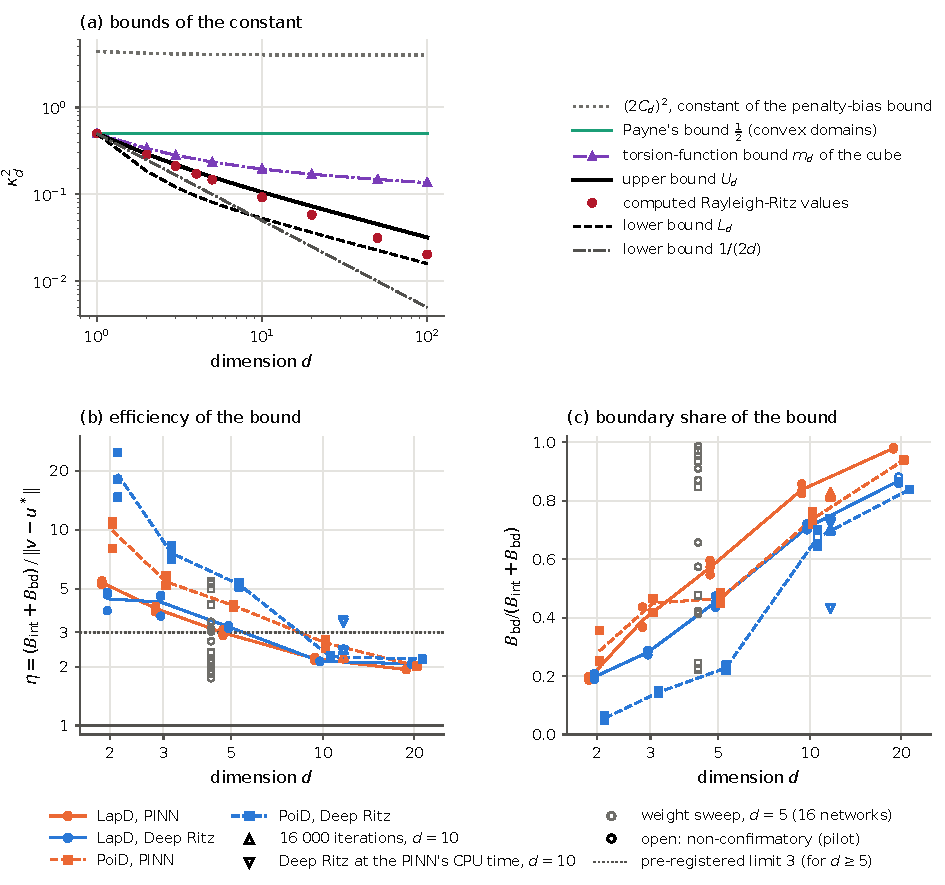
\includegraphics[width=0.78\textwidth]{s6_bound.pdf}
\caption{(a) The bounds $U_d$, $L_d$ and $1/(2d)$ of Theorem~\ref{s6_highdim:thm:kappa} on
$\kappa_d^2$, Payne's bound $\frac12$, the torsion-function bound $m_d$ of the cube
(Remark~\ref{sA_proofs:rem:steklov}), the largest computed Rayleigh quotients, and the square of the
constant $2C_d$ of Proposition~\ref{s3_methods:prop:robin}(c). (b) Efficiency $\eta$ and (c) boundary
share of the bound of Corollary~\ref{s6_highdim:cor:bound}(c) for all 88 saved networks, new
Monte-Carlo set: the main runs (lines: seed means; open markers: the seven networks seen in the
pilot), the 16\,000-iteration and equal-compute runs at $d=10$ (triangles), and the 16 networks of
the weight sweep at $d=5$ (grey, drawn slightly to the left of $d=5$). The dotted line in (b) is the
pre-registered limit 3.}
\label{s6_highdim:fig:bound}
% src: research_highdim_bound/results/theorem2_checks.json; research_highdim_bound/results/restricted_lanczos.json; research_highdim_bound/results/eval_confirm.jsonl (88 networks: main 60, long and equaltime 12, sweep 16); data/s6_highdim_torsion.json; script code/s6_highdim_bound.py (plot only)
\end{figure}

\paragraph{Relation to the literature.} Besides the classical facts recalled above (Fichera's
duality, Payne's bound, the torsion function), numerical bounds for $\delta_1$ on the square are
in~\citet{kuttler1972remarks} and~\citet{ferrero2005fourth}. Theorem~\ref{s6_highdim:thm:kappa}
adds a two-sided bound of $\kappa_d^2$ of the exact order $d^{-1/2}$ on the hypercube
(equivalently, $\kappa_d$ is of exact order $d^{-1/4}$), with an elementary proof (sine series,
the Cauchy--Schwarz inequality, partial fractions). In the literature searched for this work no
bound of $\kappa_d^2$ of the order $d^{-1/2}$ was found.
% src: research_highdim_bound/results/table_payne.tex; data/s6_highdim_torsion.json; refs.bib (bucur2011first, ferrero2005fourth, kuttler1972remarks, raulot2015sharp: annotes)
A posteriori bounds for network approximations exist in other norms and settings:
\citet{ernst2025certification} certify in the energy norm with constants not explicit in $d$;
\citet{fuhrer2025aposteriori} measure the boundary misfit in $H^{1/2}(\dOm)$ with mesh-dependent
constants; \citet{zeinhofer2025unified} work on $C^{1,1}$ domains with non-explicit constants;
in the generalisation bounds of~\citet{mishra2023generalization} the boundary misfit enters through
its square root with constants that contain norms of the network; and the bound
$\max\abs{v-\uex}\le\max_{\dOm}\abs{v-g}+\frac18\max\abs{\lap v+f}$ from the maximum principle,
explicit on the cube~\citep[Prop.~7]{mukherjee2026certification}, needs suprema, which the
Monte-Carlo losses do not estimate (on our networks its sampled value was 5.7 to 42 times the
bound of Corollary~\ref{s6_highdim:cor:bound}(c)). The closest form is in the error analysis of
residual minimisation by~\citet[App.~B, eq.~(B2)]{shin2023error}: $\norm{u}\le C(\norm{\lap
u}+\nbd{u})$, from the regularity theory of~\citet{bramble1970rayleigh}, linear in the $L^2$ norms
of the residual and of the boundary misfit as in Corollary~\ref{s6_highdim:cor:bound}(c), but on
smooth domains and with a constant that is not explicit. With Payne's constant a bound of this
form follows at once from the duality, so Corollary~\ref{s6_highdim:cor:bound}(c) is an application
of known theory with a better constant, not a new method. Imposing $v=g$
exactly~\citep{sukumar2022exact} would remove $B_{\mathrm{bd}}$ and the penalty bias; it was not
tested here. For the penalty bias, $O(1/\bet)$ is known on $C^{1,1}$ domains~\citep{muller2022},
and error bounds with extrapolation exist for the penalty finite-element
method~\citep{king1974penalty}; Proposition~\ref{sA_proofs:prop:exact} is a routine separation of
variables whose value lies in the numbers it gives on the cube.
% src: research_highdim_bound/results/decisions.json (H4: maxprinciple_over_L2bound: min 5.696, max 41.95); refs.bib (ernst2025certification, fuhrer2025aposteriori, zeinhofer2025unified, mishra2023generalization, mukherjee2026certification, shin2023error, sukumar2022exact, king1974penalty: annotes)

% -------------------------------------------------------------------------------------
\FloatBarrier
\subsection{Two cheap remedies at \texorpdfstring{$d=20$}{d = 20}}%
\label{s6_highdim:sec:remedies}

At $d=20$ and 4000 iterations neither method improves on the best affine approximation of
\Ptwo\ (Section~\ref{s6_highdim:sec:growth}); this is what is called the \emph{plateau} below: a
test error no smaller than the affine floor. Two cheap remedies suggest themselves, and neither
is new. The first, called \emph{presolve} here, writes the approximation as a fixed known part
plus a network, as in the trial solutions of \citet{lagaris1998}, with a cheap Galerkin solution
as the known part, as in Galerkin neural networks~\citep{ainsworth2021galerkin} and multi-level
networks~\citep{aldirany2024multilevel}: the fixed part is the exact minimiser of the method's own
population loss over affine functions, obtained from one $(d+1)\times(d+1)$ linear system
(Proposition~\ref{sA_proofs:prop:presolve}). The second, called \emph{lift3c}, replaces the input
$\x$ by the coordinate-wise Legendre features $P_1(t_i),P_2(t_i),P_3(t_i)$, $t_i=2x_i-1$, so that
the first layer has $3d$ inputs. Polynomial input layers trained with a PINN loss are known, for
high-frequency solutions: HOrderDNN~\citep{chang2022horderdnn}, whose first layer is a
tensor-product polynomial basis, and its coordinate-wise successor
K-HOrderDNN~\citep{zhang2025khorderdnn}, tested up to $d=10$ for PDEs and $d=50$ for function
fitting; related are the first layers of Chebyshev-basis Kolmogorov--Arnold
networks~\citep{shukla2024kan,mostajeran2025scaledcpikan} and feature-engineered or Fourier-feature
PINNs~\citep{fazliani2025safenet,wangwang2021}. Mapping the input to $[-1,1]^d$ is common practice
(the reference code of~\citet{raissi2019} does so), and the centred-input network $\mathcal N(2\x-1)$,
called \emph{lift1}, is reported as a baseline. That low-degree or low-frequency components are
learned first, which motivates both remedies, is known~\citep{rahaman2019,ghosh2022three,wangwang2021}.
What is measured here is whether either remedy removes the plateau on \Ptwo, and how each changes
the accuracy at $d=20$ on further problems, for both methods, at equal iterations and at equal CPU
time.
% src: refs.bib (chang2022horderdnn, zhang2025khorderdnn, raissi2019: annotes)

\paragraph{Design.} The test was pre-registered: hypotheses, problems, seeds 10 to 14, budgets,
metric and decision rule were fixed in a document whose hash and time were recorded in the
repository before the first counted run (no external registry was used). Both remedies had been
tried on \Pone\ and \Ptwo\ at $d=20$ in exploratory pilots with seeds 0 to 2 before the freeze, as
had the centred input (on \Pone\ at $d=20$, on \Ptwo\ up to $d=16$) and, for Deep Ritz on \Pone,
rep3, so the direction of their effects on these two problems was known. Only two problems were
held out, on which neither remedy had been tried before the test (a related ridge had been used in
an earlier pilot): the ridge \Pridge, $\uex=\cos(2s)$ with $s=d^{-1/2}\sum_i(2x_i-1)$, and
\Pcospair, $\uex=\sum_{k\le d/2}\cos(\pi x_{2k-1})\cos(\pi x_{2k})$. On \Ptwo\ the lift features
contain the solution up to $\sci{3.9}{-3}$, so \Ptwo\ is reported but excluded from the decision on
the lift. The metric is the relative $L^2$ error on the held-out test points, and the effect of an
arm is the seed-paired ratio $\rho=\errL(\text{plain})/\errL(\text{arm})$ ($\rho>1$: the arm is
more accurate). By the frozen rule a remedy \emph{helps} on a problem if, for both methods,
$\rho>1$ in at least 4 of 5 seeds with median $\rho\ge1.5$, at 4000 iterations and at equal CPU
time; it \emph{hurts} if for one method a median $\rho$ is at most $1/1.1$; it is a \emph{general
remedy} if it helps on \Pone\ and on \Pridge\ or \Pcospair\ and hurts on none of them. Two controls
were pre-registered, for Deep Ritz only: \emph{lift3u}, which spans the same functions as lift3c
but uses the uncentred feature $x_i$ in place of $P_1(t_i)$, and \emph{rep3}, the featureless input
$(t,t,t)$ with $t=2\x-1$; the centred input lift1 was added for both methods as an exploratory arm
after the frozen analysis. Three problems were added afterwards: under an addendum to the
pre-registration, the ridge \Paltridge, $\uex=\cos(\pi s'+1)$ with
$s'=d^{-1/2}\sum_i(-1)^{i+1}(2x_i-1)$ and $f=4\pi^2\uex$; and, in the descriptive second round of
the re-check, \Psinlin, $\uex=\sum_{k\le d/2}\sin(\pi x_{2k-1})\,x_{2k}$ with $f=\pi^2\uex$, and
\Pexpcos, $\uex=\sum_{k\le d/2}\ee^{x_{2k-1}}\cos x_{2k}$ with $f=0$. The full design, with the
weights, the equal-CPU budgets and the later additions, is in Supplementary
Section~\ref{S5:sec:remedies}.
% src: research_highdim_remedies/PREREG_C1.md (header: pilots with seeds 0-2; sections 2.2, 2.3, 7); notes/VERIFICATION.md (sec. 4.3, pilots before the freeze); research_highdim_remedies/PREREG_FREEZE.json; research_highdim_remedies/results/checks.json (C5_floors poisson/d20: exact_lift3); research_highdim_remedies/PREREG_C1_P5.md; research_highdim_remedies/results/check_p5_formulas.json; research_highdim_remedies/check/selftest2.json

\paragraph{Results.}
% src: research_highdim_remedies/results/decision.json (per_problem; general_lift3c); research_highdim_remedies/results/summary.json (P1-P4 presolve and lift3c); research_highdim_remedies/results/runs_main20.jsonl (ridge, ritz, seed 10); research_highdim_remedies/results/decision.json (presolve/P2 pinn: median 0.941, min 0.909, max 0.982, wins 0; centring_clause: lift3u median 0.523, 0 of 5; rep3_P1_descriptive: median 0.880, 0 of 5)
Presolve helps on \Pone\ only (median ratios 2.67 for Deep Ritz and 2.85 for the PINN, 5 of 5
seeds each; Table~\ref{s6_highdim:tab:remedies}). On \Ptwo\ it is neutral by the frozen rule
(median 1.00 for Deep Ritz) and for the PINN slightly worse in every seed (median 0.94, range 0.91
to 0.98); it changes nothing on \Pcospair, where the affine minimiser is zero
(Proposition~\ref{sA_proofs:prop:struct}), and hurts on the held-out ridge \Pridge\ (medians 0.66
and 0.79, no seed better than plain). On the four pre-registered problems lift3c is more accurate
than plain in 5 of 5 seeds for both methods, at 4000 iterations (median ratios 2.33 and 2.86 on
\Pone, 2.27 and 1.77 on \Pridge, 2.83 and 4.02 on \Pcospair, for Deep Ritz and the PINN) and at
equal CPU time, so by the frozen rule it is a general remedy on \Pone, \Pridge\ and \Pcospair.
The controls do not attribute this gain to the Legendre features on every problem
(Tables~\ref{sC_details:tab:controls} and~\ref{s6_highdim:tab:remedies5}(b)). On \Pone\ lift3u is
less accurate than plain in every seed (median 0.52), which triggered the pre-registered centring
clause, so no statement on the features is made there; no control reproduces the gain (rep3 0.88,
0 of 5 seeds better; lift1 0.92 for Deep Ritz, 2 of 5), and lift3c is 2.43 (Deep Ritz) and 1.61
(PINN) times more accurate than lift1, 5 of 5 seeds each. On \Pridge\ centring the input alone
matches the whole gain for Deep Ritz, and the PINN is more accurate with lift1 than with lift3c in
every seed (median 0.77). On \Pcospair\ lift3c also beats lift1 (2.23 and 2.39, 5 of 5), but for
Deep Ritz the featureless reparametrisation rep3 gains about as much as lift3c there, as on \Ptwo\
and \Pridge.
% src: research_highdim_remedies/results/attribution.json; research_highdim_remedies/results/summary_exploratory.json; research_highdim_remedies/results/summary.json (rep3, lift3c)
% src: research_highdim_remedies/PREREG_C1_P5.md; research_highdim_remedies/results/decision_p5.json; research_highdim_remedies/results/summary_p5.json; research_highdim_remedies/results/attribution.json (P5 pinn lift1_vs_plain 1.287, 5/5)
\Paltridge\ was run with the study's own code under the addendum, frozen before these runs; it is
not a blind test, since three seeds of the re-check had already shown the sign of the lift effect
on it. There the lift hurts (Deep Ritz median ratio 0.59 at 4000 iterations and 0.32 at equal CPU
time, 0 of 5 seeds better; PINN 0.88 and 0.72), and so does presolve (Deep Ritz 0.73, PINN 0.83),
whereas the centred input alone makes the PINN more accurate (1.29, 5 of 5). By the extended rule
of the addendum neither presolve nor lift3c is a general remedy on the five problems.
% src: data/s6_highdim_remedies_recheck.json (P6 lift1/lift3c 1.011; P7/ritz/d20: plain_err 0.02504-0.02532, presolve/4000 median 4.507); research_highdim_remedies/check/selftest2.json (P7_floor_affine 0.0224)
In the second round of the re-check (Deep Ritz, three seeds, a different implementation,
descriptive) the gain of the lift on \Psinlin\ is again matched by centring the input, and
\Pexpcos\ is on the plateau ($\errL=0.025$, affine floor 0.022), which presolve leaves (median
ratio 4.51).

\paragraph{What this shows and what it does not.} At $d=20$, with this network, optimiser,
schedule and these weights, the accuracy of both methods depends strongly on how the input enters
the first layer, in a way that differs between problems; no single mechanism (centring the input or
the polynomial features) accounts for it on every problem.
% src: research_highdim_remedies/results/summary.json (plain, d20); research_highdim_remedies/results/summary_p5.json (plain, d20); research_highdim_remedies/results/checks.json (C5_floors: test_affine); research_highdim_remedies/results/checks_p5.json (C5); data/s6_highdim_remedies_recheck.json (P6/ritz/d20 plain_err 0.0997-0.1155, P7/ritz/d20 plain_err 0.02504-0.02532); research_highdim_remedies/check/selftest2.json (P6_floor_affine 0.1716, P7_floor_affine 0.0224)
Of the five problems of the study only \Ptwo\ is on the plateau after 4000 iterations
(plain $\errL=0.126$ for Deep Ritz and $0.145$ for the PINN, against the affine floor $0.119$ on
the test set), and of the two of the re-check only \Pexpcos; on the others plain already ends
below the affine floor, so there the comparison is
one of accuracy at a fixed budget, not of escaping a plateau.
% src: research_highdim_remedies/results/summary.json (P2/d20: ritz lift3c, lift3u, rep3; pinn lift3c); research_highdim_remedies/results/summary_exploratory.json (P2/d20/ritz/lift1/4000: min 0.0699, max 0.0914; P2/d20/pinn/lift1/4000: min 0.0670, max 0.0796); research_highdim_remedies/results/checks.json (C5_floors poisson/d20: test_affine 0.1193, exact_lift3 3.9e-3); research_highdim_remedies/results/attribution.json and Table s6_highdim:tab:remedies5(b) (P2 lift1/lift3c: 4.22 Deep Ritz, 7.51 PINN, 5/5)
On \Ptwo\ presolve does not leave the plateau. lift3c does, for both methods and in every seed.
For Deep Ritz the gain cannot be attributed to its features, although they contain the solution of
\Ptwo\ up to $\sci{3.9}{-3}$: the featureless control rep3 is more accurate still (median ratio
8.10 against 6.59) and lift3u gains as much (6.71). The centred input alone (lift1, exploratory)
already ends below the affine floor in every seed for both methods ($\errL=0.070$ to $0.091$ for
Deep Ritz and $0.067$ to $0.080$ for the PINN, against 0.119), but with less gain than lift3c, which
is 4.22 times (Deep Ritz) and 7.51 times (PINN) more accurate than lift1 in median, 5 of 5 seeds
each (Table~\ref{s6_highdim:tab:remedies5}(b)); for the PINN, for which no featureless control was
run, the features thus add to centring on \Ptwo. At this budget the plateau of \Ptwo\ is therefore not robust to centring
the input, which is common practice. As a remedy the result is negative: neither remedy is general,
and neither is new as a method. What is added is a measurement of both, for the PINN and Deep Ritz
side by side, at equal iterations and at equal CPU time, on two problems held out from the pilots
and three added later, with two pre-registered controls for Deep Ritz (lift3u, rep3) and an
exploratory centred-input arm for both methods.

% -------------------------------------------------------------------------------------
\subsection{Comparison with published results}\label{s6_highdim:sec:limits}

% src: research_highdim/results/extensions.json (long, laplace, d = 10, 16 000 iterations: pinn 5.590e-3, 5.928e-3, 6.130e-3; ritz 6.830e-3, 7.438e-3, 7.568e-3); refs.bib (eyu2018, annote)
For \Pone\ at $d=10$, \citet{eyu2018} report a relative $L^2$ error of about 0.4 per cent after
50\,000 iterations with a 671-parameter network and $\bet=10^3$. Our mean errors at $d=10$ after
16\,000 iterations are 0.59 per cent (PINN) and 0.73 per cent (Deep Ritz), with best seeds at 0.56
and 0.68 per cent, for a different network, sampling and schedule. The orders of magnitude agree;
we do not claim to reproduce their number. For the Neumann example whose solution \Ptwo\ shares,
they report 1.3 per cent at $d=5$ and 1.9 per cent at $d=10$ with the Ritz method and no boundary
penalty; equation, boundary condition, network and budget differ from ours, so this is not a
like-for-like comparison with Table~\ref{s6_highdim:tab:p2}.
% src: refs.bib (chen2020comparison, annote: abstract of arXiv:2005.04554, checked 2026-10-01)
\citet{chen2020comparison} set the deep Galerkin method~\citep{sirignano2018}, whose loss is the
residual least-squares loss of a PINN, against the Deep Ritz method on elliptic problems with
boundary conditions imposed by penalty. They report that Deep Ritz can outperform the residual
method even for smooth solutions, with a clear dependence on the dimension, that the residual
method can outperform Deep Ritz for solutions of low regularity, and that imposing the boundary
condition exactly, where that is possible, gives a better solution and an easier training. Our
finding that the PINN is the more accurate method per iteration for $d\le10$ on two smooth
problems is therefore not a general ranking, and it does not contradict theirs: networks,
sampling, penalty weights and budgets differ, and our own ranking changes with what is counted
and with the budget. What the two studies have in common is that neither loss dominates the
other.

% =====================================================================================
% sections/s7_pitfalls.tex -- Two implementation pitfalls, demonstrated on minimal examples.
% Demonstration of Section 7.1: code/s7_pitfalls.py -> data/s7_pitfalls_autograd.json,
%   figures/s7_pitfalls.pdf; with --passes 1500 -> data/s7_pitfalls_autograd_1500passes.json.
% Demonstration of Section 7.2: research_benchmark/scripts/run_oneface.py
%   -> research_benchmark/results/oneface_laplace3d.json.
% Details, the listing and the figure: sections/S6_pitfalls.tex.  All "% src:" paths are relative
% to the root of the repository.
% =====================================================================================
\section{Two implementation pitfalls, demonstrated on minimal examples}\label{s7_pitfalls:sec}

A PINN can reach a small training loss and still be far from the solution for reasons that
have nothing to do with the optimiser or the points. This section demonstrates two such
reasons on minimal, released examples. Neither depends on seeds or budgets, and each is caught
by a cheap test that we recommend in Section~\ref{s8_discussion:sec:checklist}.

% -------------------------------------------------------------------------------------
\subsection{A residual that automatic differentiation makes identically zero}%
\label{s7_pitfalls:sec:autograd}

A tempting way to obtain $u_{tt}$ in PyTorch is to differentiate $u_t$ with respect to the
column \code{x[:, 0]} of the input tensor \code{x}. Indexing creates a new tensor, and $u_t$ was
computed from \code{x}, not from that slice, so reverse-mode differentiation~\citep{paszke2019}
finds no path between the two. Without \code{allow_unused=True} the call raises an error; with
it the call returns \code{None}, and code that replaces a missing derivative by zeros turns the
residual into the constant zero, which gives the loss neither a value nor a gradient. The correct
pattern differentiates with respect to the whole input and indexes the result
(Listing~\ref{s7_pitfalls:lst:autograd}).
% src: data/s7_pitfalls_autograd.json (autograd_demo; operator_unit_test_float64: faulty 0.0 and 0.0; correct 3.55e-15 and 19.61)
A unit test exposes the fault at once: in double precision on 2000 random points the faulty
operator for the wave equation $u_{tt}=\lap u$ returns exactly 0 both for the solution of \PWtwo\
and for the non-solution $\ee^{-t}\sin\pi x\sin\pi y$, whereas the correct operator returns at
most $\sci{3.6}{-15}$ for the former and values up to 19.6 for the latter.

% src: data/s7_pitfalls_autograd.json (training: steps 23550, none_returns 70650 of 70650 calls, max_pde_term_over_all_steps 0.0, loss 0.1011 -> 1.1007e-04; heldout_21x81x81: 1.3507 vs exact, 0.0247 vs target; slices at t = 0, 1: amplitude 0.98110, 0.36431)
Training gives no warning. We trained a 3--50--50--1 tanh network on the domain of \PWtwo\ with
a loss made of the faulty residual, a data term that prescribes $\ee^{-t}\sin\pi x\sin\pi y$ at
10\,000 random space--time points and a zero boundary term at 400 points of the spatial boundary at
$t=0$ (batches of 64, \Adam\
with learning rate $10^{-3}$, seed 0, 23\,550 iterations). The PDE term was exactly 0 at every
iteration (all 70\,650 second-derivative calls returned \code{None}), while the loss fell from
0.10 to $\sci{1.1}{-4}$. The network fitted the data term (relative distance 0.025 on the held-out
grid of \PWtwo) and followed its decay, with mode amplitudes 0.981 and 0.364 at $t=0$ and 1; its
relative distance from the solution of \PWtwo\ is 1.35. The network thus follows whatever the data
term prescribes; a correct residual would have penalised this data term, which is not a wave:

\begin{proposition}[A decaying mode is not a wave solution]\label{s7_pitfalls:prop:notwave}
\StmtNotWave
\end{proposition}

% src: data/closed_forms.json (wave2d.rel_L2_target_vs_exact_ut0_zero = 1.3800); data/s7_pitfalls_autograd.json (heldout_21x81x81.rel_L2_target_vs_exact = 1.3528); data/s7_pitfalls_autograd_1500passes.json (training: steps 235500, max_pde_term_over_all_steps 0.0, loss 0.1011 -> 5.61e-06; heldout_21x81x81: 1.3532 vs exact)
\noindent On the held-out grid, which has 21 time levels, the ratio of part~(b) is 1.353. With ten
times as many iterations nothing changes in kind: the PDE term is exactly 0 at all 235\,500
iterations, the loss falls to $\sci{5.6}{-6}$, and the distance from the solution is 1.35. Three
guards would each catch the fault: never pass \code{allow_unused=True} in a residual; assert that
every derivative is not \code{None}; and unit-test each residual operator on an exact solution
\emph{and} on a non-solution. The last is decisive, since a test on an exact solution alone is
passed by the zero operator.

% -------------------------------------------------------------------------------------
\subsection{A small loss does not imply a unique solution}\label{s7_pitfalls:sec:oneface}

A boundary-value problem with too few conditions has a whole family of solutions, and a PINN
trained on it may converge to any of them. The Laplace equation in the cube with data on one face
is the simplest example.

\begin{proposition}[A Laplace problem with data on one face only]\label{s7_pitfalls:prop:nonunique}
\StmtNonunique
\end{proposition}

% src: research_benchmark/results/oneface_laplace3d.json (oneface_laplace3d.rows: rel_l2 1.616, 12.51, 13.22, 7.275, 1.633; final_bc_loss 2.7e-04..2.2e-03, final_pde_loss 4.1e-04..7.9e-04; mean_abs_u_face_x0 0.267, 2.62, 2.65, 1.45, 0.259); research_benchmark/scripts/run_oneface.py
We trained five seeded $2\times100$ tanh networks on this problem, with the residual on the closed
$21^3$ grid of the cube and the datum on its 441 points with $x=\pi$ (AdamW~\citep{loshchilov2019}
with learning rate $10^{-3}$ and its default weight decay, 2000 iterations). Both loss terms end between $\sci{2.7}{-4}$ and $\sci{2.2}{-3}$ in
every run, and the five networks are five different, nearly harmonic functions: their relative
$L^2$ distance from the solution of \PLthree, which has the same datum and zero data on the other
five faces, is 1.62, 12.51, 13.22, 7.28 and 1.63, and the mean of $\abs{\unet}$ on the face $x=0$
is 0.27, 2.62, 2.65, 1.45 and 0.26 (Figure~\ref{s7_pitfalls:fig:demo}), in line with part~(c) of
the proposition.
% src: verify_research_benchmark/v_oneface.json (oneface|0..2: rel_l2 1.589, 12.84, 13.36); verify_research_benchmark/v_oneface.py
A re-run of seeds 0 to 2 with the separately written code \textsf{V-bench}
(Section~\ref{s3_methods:sec:verif}) gave the distances 1.59, 12.84 and 13.36. Nothing in such a
loss selects one solution, so the outcome depends on the initial weights. Count the conditions before training and say why the solution is unique; and run
more than one seed: an answer that changes with the seed while the loss stays comparably small is
the symptom.

The settings of the two demonstrations are arbitrary, were not tuned and differ from the
protocol of Section~\ref{s3_methods:sec}. The mechanism of each, a residual that is identically
zero and a loss that does not determine the solution, does not depend on them; the particular
numbers do.

% =====================================================================================
% sections/s8_discussion.tex -- Discussion, limitations and conclusion.
% No computation and no new numbers: every figure quoted here is stated or tabulated in
% an earlier section.  The "% src:" comments name the underlying file (paths relative to
% the root of the repository).
% =====================================================================================
\section{Discussion, limitations and conclusion}\label{s8_discussion:sec}

\subsection{What the evidence supports}\label{s8_discussion:sec:evidence}

Findings (1) to (5) are ordered by the strength of their evidence, strongest first; (6) and (7)
concern Sections~\ref{s6_highdim:sec:bound} and~\ref{s6_highdim:sec:remedies}, and (8) the
reporting of errors.

\begin{enumerate}[label=(\arabic*),leftmargin=*]
% src: data/s7_pitfalls_autograd.json (operator_unit_test_float64; training.max_pde_term_over_all_steps 0.0); research_benchmark/results/oneface_laplace3d.json
\item \emph{Two implementation faults give a small loss and a wrong answer.} A residual made
identically zero by a misused automatic-differentiation call, and a boundary-value problem with data
on one face of six, each gave a small training loss and a wrong answer (Section~\ref{s7_pitfalls:sec}): in the
first the network follows whatever the data term prescribes, which a correct residual would have
penalised. Neither fault depends on seeds or budgets, and each is exposed by a cheap test.
% src: research_benchmark/results/tables.md (T2: 175 of 175); data/s4_lowdim_numbers.json (lbfgs_vs_logged_adam_iterates_it1500_3000); verify_research_benchmark/v_summary.out (39 of 40); data/s5_hard_wave2d_long.json (summary.per_seed: adam_lbfgs_rel_l2 5.7e-3 to 9.3e-3)
\item \emph{An \LBFGS\ phase is the most effective change tested.} At equal iteration count it
lowered the held-out error in all 175 pairs (39 of 40 in the verification code), by about one order
of magnitude on \PH\ and \PLtwo\ even against the best logged \Adam\ iterate, and a longer phase took
\PWtwo\ below one per cent (Sections~\ref{s4_lowdim:sec:optimiser} and~\ref{s5_hard:sec:w2}). The
\Adam\ arm was not tuned.
% src: research_benchmark/results/tables.md (T3, T6; T3 laplace2d adam resample 6.36, 0/10, the largest ratio of the table); data/s4_lowdim_gridcontrol.json (column against placebo 0.19, 10 of 10); verify_research_benchmark/v_summary.out
\item \emph{The choice among space-filling point sets is secondary.} No strategy is best on every
problem; the largest effect after the \LBFGS\ phase, a fourfold penalty of the cell-centred grid on
\PH, is caused by the absence of residual points next to the initial line
(Table~\ref{s4_lowdim:tab:gridcontrol}). Adaptive sampling brought no detectable gain at our budget,
and redrawing the points at every iteration hurt under \Adam\ alone (on \PLtwo\ by a factor 6.4,
the largest penalty of any strategy in the benchmark) but not after the \LBFGS\ phase (Section~\ref{s4_lowdim:sec:strategy}).
% src: research_benchmark/results/benchmark_runs.csv (wave1d: 50 runs, 0.414 to 0.512); data/s5_hard_wave1d_long.json (summary.per_seed: 0.337 to 0.381); data/s5_hard_cost.json (summary: ratio_smallest_of_all_measurements 475.6, ratio_B_range 1.9e3 to 1.3e5)
\item \emph{At the sizes and budgets used, the unit-weight PINN does not solve the two-mode wave
problem, and finite differences are far faster.} All 50 runs on \PWone\ ended between 41 and 51 per
cent error and the longer runs between 34 and 38 per cent, although \citet{rathore2024} report a few
per cent with wider networks, more points and a tuned schedule. A second-order finite-difference solve
was at least as accurate as the best PINN on all five problems and faster by a factor of more than
400 in every timing (smallest measured ratio $\sci{4.8}{2}$; Section~\ref{s5_hard:sec:fd}), as \citet{grossmann2024} found against finite
elements.
% src: research_highdim/results/summary.csv; research_highdim/results/extensions.json; data/s6_highdim_long_d20.jsonl; data/s6_highdim_robin_bias.json (against_trained_networks.beta_100_16000_iterations: bias_over_gap 1.048, 0.654); data/s6_highdim_bound_numbers.json (recheck_r2: P1_ritz_eqcpu_d20, P1_pinn_d20)
\item \emph{In higher dimension the ranking of PINN and Deep Ritz depends on what is counted.} Per
iteration the PINN was the more accurate for $d\le10$ and, with 16\,000 iterations, at $d=20$; at
equal compute Deep Ritz was the more accurate (at $d=10$, and at $d=20$ for \Pone\ in a descriptive
re-check with three seeds; Sections~\ref{s6_highdim:sec:equal-its}--\ref{s6_highdim:sec:compute}).
On \Pone\ the lead of the PINN at the larger budget is of the size of the penalty bias of Deep Ritz
(Section~\ref{s6_highdim:sec:weights}). As in \citet{chen2020comparison}, neither loss dominates.
% src: data/s6_highdim_bound_numbers.json (n_networks_bound_valid; eta_d10_d20_all_networks; eta_by_d_all_networks; recheck_r2: pairs_ranked_like_error_equal_iterations 4/9); research_highdim_bound/results/decisions.json (H2: 21 of 57, max 5.456)
\item \emph{On the unit cube the error of a network is bounded by the two population terms of its
loss, but the bound is loose at small $d$.} The constant of the harmonic extension is of exact order $d^{-1/4}$
(Theorem~\ref{s6_highdim:thm:kappa}); the bound of Corollary~\ref{s6_highdim:cor:bound} held on all
133 networks evaluated, with efficiency 1.92 to 3.44 at $d=10$ and 20, but the pre-registered target
of an efficiency of at most 3 for $d\ge5$ failed (21 of 57 networks), and at $d=2$ the efficiency
reached 24.8. It is a certificate, not an error estimator. A bound of this form already follows from
Payne's classical constant; the theorem adds the order in $d$.
% src: research_highdim_remedies/results/decision.json; research_highdim_remedies/results/decision_p5.json; research_highdim_remedies/results/summary.json (P2/d20 lift3c, rep3; presolve and lift3c medians); research_highdim_remedies/results/summary_exploratory.json (P2/d20 lift1); research_highdim_remedies/results/attribution.json (P2 lift1/lift3c); research_highdim_remedies/results/summary_p5.json (P5/d20 presolve, lift3c); research_highdim_remedies/results/checks.json (C5_floors poisson/d20: exact_lift3 3.9e-3)
\item \emph{Neither cheap remedy is general at $d=20$.} By the pre-registered rule the Legendre
features (lift3c) were a general remedy on the four pre-registered problems, but they and the fixed
affine part were less accurate than plain on \Paltridge, which was added afterwards and was not a
blind test; the affine part also hurt on \Pridge. The features left the plateau of \Ptwo, whose
solution they contain up to $\sci{3.9}{-3}$, as did the centred input alone (exploratory, with
less gain) and, for Deep Ritz, the featureless control rep3 (with more); how much of each gain the
features explain differs between problems (Section~\ref{s6_highdim:sec:remedies}).
% src: data/closed_forms.json (floors); data/s4_lowdim_timeslices.json (summary: n_seeds_slice_t1_above_1 = 10 in all four cells)
\item \emph{How an error is reported changes the conclusion.} A relative $L^2$ error needs the error
of a trivial predictor beside it (Proposition~\ref{s2_problems:prop:floors}), and for a decaying
solution the space--time error hides the late slices: all 40 runs of Section~\ref{s4_lowdim:sec:timeslice}
are more than 100 per cent in error on the slice $t=1$, at a space--time error of about 0.1 per cent
after \AdamLBFGS.
\end{enumerate}

\subsection{A checklist for small PINN studies}\label{s8_discussion:sec:checklist}

\begin{enumerate}[label=\arabic*.,leftmargin=*]
\item Unit-test every residual operator on an exact solution and on a non-solution, and never
let a missing derivative default to zero (Section~\ref{s7_pitfalls:sec:autograd}).
\item Count the initial and boundary conditions and say why the solution is unique
(Section~\ref{s7_pitfalls:sec:oneface}).
\item Fix and report seeds, at least five, preferably ten, per configuration, and compare
paired by seed.
\item Report held-out relative errors, not training losses, per time slice for evolution
problems (Section~\ref{s4_lowdim:sec:timeslice}), with the error of a trivial predictor beside
them (Proposition~\ref{s2_problems:prop:floors}).
\item Run a classical baseline on the same evaluation set, after checking it against an
exact solution (Section~\ref{s5_hard:sec:fd}).
\end{enumerate}

\subsection{Limitations}\label{s8_discussion:sec:limitations}

\emph{Budgets.} The benchmark uses 256 to 1024 interior points and 3000 iterations. The
strategy effects belong to this scarce-point regime.

\emph{Statistics.} \PWone, \PWtwo\ and \PLthree\ have five seeds, for which the paired
test cannot go below $p=0.0625$, so ``no significant difference'' is weak evidence there.
The $p$-values are not corrected for multiple comparisons, and the rule by which we call
an effect significant (all ten seeds agree; Section~\ref{s3_methods:sec:stats}) was fixed
after the results were known.
% src: notes/VERIFICATION.md (sec. 2.5, caveat 2)

\emph{Verification.} The re-checks were made with separately written code within the same
project, on the same machine and library versions; they are not a replication by a third
party. The longer runs, the control experiments, the time-slice result, the 16\,000-iteration
runs at $d=20$ and the demonstration of Section~\ref{s7_pitfalls:sec:autograd} rest on the code of
the experiments alone (Section~\ref{s3_methods:sec:verif}).

\emph{Scope.} All problems are linear with constant coefficients on boxes, and their
solutions are smooth except at the discontinuous data of \PLthree. Each problem has one
tanh architecture, and Sections~\ref{s4_lowdim:sec} and~\ref{s5_hard:sec} use unit loss
weights. Uniqueness is proved in a stated class (classical solutions; for \PLthree, the
solutions that attain the datum in mean square); continuous dependence on the data is not
proved.

\emph{Unfinished problems.} \PWtwo\ and \PLthree\ are not converged at 3000 iterations.
The longer runs on \PWtwo\ (three seeds, one strategy) ended on the tolerance of the
optimiser in single precision, below one per cent but not on a plateau
(Section~\ref{s5_hard:sec:w2}). \PWone\ is not solved at the network size and budgets
used (Section~\ref{s5_hard:sec:w1}).
% src: research_benchmark/results/runs/wave2d_s0-5.json, laplace3d_s0-5.json (median held-out error of the 25 runs still falling between iterations 2750 and 3000: 5.81e-2 to 4.58e-2 and 4.56e-2 to 4.27e-2)
% src: data/s5_hard_wave2d_long.json (summary.per_seed: stop, adam_lbfgs_test_ratio_9500_over_8500); notes/VERIFICATION.md (sec. 2.5, caveat 6)

\emph{Implementation.} Most multi-seed runs used single precision on a GPU backend. A stack
repeated on the same machine reproduces its results bit for bit, but the result of one
network depends on the stack in which it is trained (its size and composition; the mechanism,
presumably rounding, was not investigated; Supplementary Section~\ref{sC_details:sec:repro}); other hardware was not tested. The \LBFGS\ of these runs
is a custom stacked implementation whose final errors were 4 to 10 per cent above those of the
reference optimiser, in geometric mean, in the validation of
Supplementary Section~\ref{sC_details:sec:validation}.
% src: research_benchmark/results/validate_batched.json (ratio stacked/single: geometric mean 1.10 on heat1d, 1.04 on laplace2d); notes/VERIFICATION.md (sec. 2.5, caveats 3 and 4)

\emph{Timings} come from three measurements on a loaded shared machine, with different
drivers, and are good to an order of magnitude only.
% src: data/checks/machine_load.json; notes/VERIFICATION.md (sec. 2.3, item 7; sec. 3.3, item 4)

\emph{Dimension study.} There are three seeds per cell, which understates the spread
(Table~\ref{s6_highdim:tab:vdim}) and allows no test, and no network was trained for
$d>20$. One architecture and one learning-rate schedule serve every $d$; the schedule
itself arrests the descent, so the errors at a fixed budget include its effect. The
weights were tuned at $d=5$ with one run per value, and $\lam$ and $\bet$ are normalised
differently in $d$ (Remark~\ref{s3_methods:rem:consistent}). Both solutions are simple in
structure, a sum of products of pairs of coordinates and a sum of functions of one
coordinate, and that of \Ptwo, with zero normal derivative, favours Deep Ritz. Boundary
conditions are imposed by penalty only. The inputs of the dimension study are not centred;
% src: research_highdim_remedies/results/summary_exploratory.json (P1, P2 at d = 20: paired plain/lift1 medians 0.92, 1.78, 1.57, 1.95; per seed 0.83 to 2.27); research_highdim_remedies/results/summary.json (plain)
centring alone (exploratory, Section~\ref{s6_highdim:sec:remedies}) changes the errors at $d=20$
and 4000 iterations by median factors of 0.92 to 1.95 (0.83 to 2.27 per seed), makes the PINN more
accurate than Deep Ritz on \Pone\ and takes both methods below the affine floor on \Ptwo. The 16\,000-iteration runs exist for $d=10$ on
\Pone\ and for $d=20$ only, and the equal-compute comparison for $d=10$ and, in the re-check,
for \Pone\ at $d=20$ with three seeds.
% src: notes/VERIFICATION.md (sec. 3.4; sec. 3.3, item 6)

\emph{Stability constant and remedies.} Theorem~\ref{s6_highdim:thm:kappa} and the bound of
Corollary~\ref{s6_highdim:cor:bound} are proved for the unit cube only, and whether $U_d$ is sharp
is open; the bound holds for the exact norms and was evaluated with Monte-Carlo estimates of them,
with margins of at least 75 standard errors on the 88 saved networks and 92 on the 21 networks of
the second round of the re-check; for the 24 networks of its first round (efficiency at least 1.97)
no standard errors were recorded. The remedies were tested with the network, optimiser,
schedule and weights of Section~\ref{s6_highdim:sec}, with five seeds at $d=20$ and three at $d=5$
and $10$, and with CPU-time budgets measured on a loaded shared machine. Both remedies, the centred
input and, for Deep Ritz on \Pone, rep3 had been tried on \Pone\ and \Ptwo\ in exploratory pilots
before the freeze, so their direction on these two problems was known and only \Pridge\ and
\Pcospair\ were held out; the pre-registered controls lift3u and rep3 were run for Deep Ritz only;
\Paltridge\ was not a blind test; and the second round of the re-check, which added \Psinlin\
and \Pexpcos, is descriptive, and three planned cells of it were not run (Supplementary
Section~\ref{S5:sec:remedies}).
% src: research_highdim_bound/results/decisions.json (H1: min_z_D hd 75.49); data/s6_highdim_bound_numbers.json (recheck_r2: min_z 92.57; n_networks_bound_valid: recheck_round1_eta_range from 1.974); research_highdim_bound/check/out/c4_fresh.jsonl (no standard-error fields); data/s6_highdim_remedies_recheck.json (missing_runs_of_plan; load1_range); notes/VERIFICATION.md (sec. 4.3, pilots before the freeze)

\subsection{What was not tried}\label{s8_discussion:sec:nottried}

Apart from the two cheap remedies of Section~\ref{s6_highdim:sec:remedies}, none of the
published remedies for the failures seen here was tried: adaptive loss
weighting \citep{wangteng2021,wangyu2022}, causal training \citep{wangsankaran2024},
Fourier-feature inputs \citep{wangwang2021}, or trial functions that satisfy the initial
and boundary conditions exactly \citep{lagaris1998,sheng2021,sukumar2022exact}; on the cube the
last would also remove the boundary term of the bound of Section~\ref{s6_highdim:sec:bound} and
the penalty bias. For Deep Ritz we tried neither continuation in $\bet$ nor a consistent boundary
treatment of Nitsche type~\citep{nitsche1971}, which exists in a neural
version~\citep{liao2021nitsche}. Non-linear and variable-coefficient equations, domains other than
boxes, and more seeds are the natural next steps.

\subsection{Conclusion}\label{s8_discussion:sec:conclusion}

We posed eight linear problems so that each has a unique solution in a stated class
(Proposition~\ref{s2_problems:prop:unique}), measured seeded held-out errors of PINNs and the Deep
Ritz method against exact solutions and, in low dimension, finite-difference baselines, and checked
the benchmark and the dimension study in part with separately written code. On these problems an \LBFGS\
phase mattered most; after it, and once the strip next to the initial line had residual points, the
collocation strategy changed the error by at most about a factor of two in geometric mean
($\Nr\ge256$); a classical solver was far faster; a unit-weight PINN of the size used did not solve
the two-mode wave problem; and whether the PINN or Deep Ritz is ahead in higher dimension depended
on the budget, on what is counted, on the input scaling and, on the Laplace problem, on the penalty
bias. On the unit cube a classical stability constant now has explicit two-sided bounds of the right
order in $d$; with it, as already with Payne's classical constant, the two population terms of the
PINN loss bound the $L^2$ error of any $C^2$ network, and the theorem sharpens that bound. The bound held on every network
evaluated but is loose. Of two cheap remedies at $d=20$, the fixed affine part did not remove the
plateau of the Poisson problem, and the Legendre features, which contain its solution up to 0.4 per
cent, did, as did centring the input alone (exploratory); neither remedy improved the accuracy on
every problem. Finally, the two pitfalls of
Section~\ref{s7_pitfalls:sec} show that a small training loss is not evidence of a correct solution;
each is caught by an entry of the checklist above.


% ---------------------------------------------------------------------- end matter ---
\phantomsection\pdfbookmark[1]{Data and code availability}{bm:code}
\section*{Data and code availability}
All code, raw results, figure scripts and the \LaTeX{} sources of this article and of its
Supplementary Material are available at\\
\url{https://github.com/zhouyi-xiaoxiao/pinn-diffusion-wave-laplace}. Every figure is
produced by a script from the stored per-run results in that repository, and every table
of results is generated from them by a script or, for the tables assembled in the text,
checked against them by one; the file \texttt{reproduce.md} gives the script and the exact
command for each, and \texttt{notes/VERIFICATION.md} describes how the results were
checked. The script \texttt{code/\allowbreak check\_headline\_numbers.py} checks the numbers
of the abstract against the stored results. All runs are seeded. The analyses of
Sections~\ref{s6_highdim:sec:bound} and~\ref{s6_highdim:sec:remedies} are in the folders
\texttt{research\_\allowbreak highdim\_\allowbreak bound} and
\texttt{research\_\allowbreak highdim\_\allowbreak remedies}, each with its pre-registration
documents, scripts, stored results and the scripts and outputs of its re-checks.
% src: research_highdim_bound/results/inventory.json (88 rows with sha256); verify_research_highdim/results/v_determinism.txt (seven runs bit for bit)
Trained networks are not included. This applies also to the 88 networks on which the bound of
Section~\ref{s6_highdim:sec:bound} was evaluated: their SHA-256 hashes, recorded before the
evaluation, and the outputs of the evaluation are included, and the training scripts retrain the
networks (on the machine used, seven runs of the dimension study were repeated bit for bit), so
the evaluation can be repeated only on retrained networks.

\phantomsection\pdfbookmark[1]{Acknowledgements}{bm:ack}
\section*{Acknowledgements}
This article develops a project report written in 2024 during an exchange year at the Hong Kong University of Science and Technology.

\phantomsection\pdfbookmark[1]{References}{bm:refs}
\bibliographystyle{plainnat}
\bibliography{refs}

\end{document}
